% =====================================================================
%  Full-Waveform Inversion -- Volume 2: Intermediário
%  Compile com:  xelatex fwi_nivel2_intermediario.tex  (duas vezes)
% =====================================================================
\documentclass[11pt,a4paper,oneside]{report}
\usepackage{fwiestilo}

\renewcommand{\nivelnum}{2}
\renewcommand{\nivelnome}{Intermedi\'ario}

\begin{document}

\capafwi
{As dedu\c{c}\~oes completas, os algoritmos e as contas\\que voc\^e precisa
fazer antes de rodar}
{``Um dado sint\'etico errado quase nunca vem com aviso.\\Ele vem bonito.''}
{12 cap\'itulos $\cdot$ mesma espinha dorsal dos tr\^es volumes}

\tableofcontents
\cleardoublepage

% =====================================================================
\chapter*{Como usar este volume}
\addcontentsline{toc}{chapter}{Como usar este volume}
\markboth{COMO USAR}{}

Esta cole\c{c}\~ao conta a mesma hist\'oria tr\^es vezes, com profundidade
crescente. Os doze cap\'itulos s\~ao os mesmos nos tr\^es volumes, na mesma
ordem, tratando dos mesmos t\'opicos: o que muda \'e a complexidade e a
completude, nunca o escopo.

\begin{center}
\begin{tabular}{@{}llp{7.4cm}@{}}
\toprule
\textbf{Volume} & \textbf{N\'ivel} & \textbf{O que faz} \\
\midrule
1 & Introdut\'orio & As ideias, as figuras e as conclus\~oes. As f\'ormulas
s\~ao \emph{lidas}, n\~ao derivadas. \\
\textbf{2} & \textbf{Intermedi\'ario} & \textbf{Este volume.} Todas as
dedu\c{c}\~oes, as vers\~oes discretas, os algoritmos, as contas de
dimensionamento e exerc\'icios resolvidos. \\
3 & Avan\c{c}ado & Formula\c{c}\~ao em espa\c{c}os de fun\c{c}\~oes, teoria de
espalhamento, estrutura da Hessiana, multipar\^ametro, funcionais
alternativos, incerteza. \\
\bottomrule
\end{tabular}
\end{center}

\section*{Para quem \'e}

Para quem vai \textbf{escrever} ou \textbf{operar} um c\'odigo de FWI. Ao
final deste volume voc\^e deve ser capaz de: dimensionar uma simula\c{c}\~ao
sem chute; derivar e implementar o gradiente adjunto; provar que o seu
gradiente est\'a certo; escolher e ajustar um otimizador; montar um fluxo
multiescala; e diagnosticar um resultado ruim pela causa, n\~ao por tentativa
e erro.

\textbf{Pr\'e-requisitos:} c\'alculo de v\'arias vari\'aveis, no\c{c}\~oes de
equa\c{c}\~oes diferenciais parciais, \'algebra linear, e alguma
familiaridade com m\'etodos num\'ericos. N\~ao \'e preciso ter visto
c\'alculo variacional --- o pouco que \'e usado est\'a derivado no
Cap\'itulo~\ref{cap:adjunto}.

\section*{Como o volume est\'a organizado}

\begin{center}
\begin{tabular}{@{}llp{7.9cm}@{}}
\toprule
\textbf{Parte} & \textbf{Caps.} & \textbf{Assunto} \\
\midrule
I   & 1--4   & O problema direto: de onde vem a equa\c{c}\~ao, como
discretiz\'a-la sem estragar a f\'isica, o que fazer com as bordas \\
II  & 5--10  & O problema inverso: funcional, gradiente, verifica\c{c}\~ao,
otimiza\c{c}\~ao, fluxo completo, regulariza\c{c}\~ao \\
III & 11--12 & Os limites da f\'isica adotada e o diagn\'ostico \\
\bottomrule
\end{tabular}
\end{center}

Marcas como esta apontam para os outros n\'iveis:

\ponte{N\'ivel 1, Cap.\ 6}{a mesma ideia contada sem matem\'atica, se a
dedu\c{c}\~ao a seguir ficar abstrata demais.}
\ponte{N\'ivel 3, §6.2}{a mesma dedu\c{c}\~ao em espa\c{c}os de
fun\c{c}\~oes, com a derivada de Fr\'echet e os termos de fronteira
tratados com rigor.}

\begin{atencao}[Sobre os n\'umeros deste volume]
Valores num\'ericos, tabelas medidas e figuras fotogr\'aficas v\^em do
c\'odigo do curso (\arq{aulas/}, \arq{fwikit/}), executado no ambiente
descrito no \arq{README.md} --- n\~ao foram copiados de livro. Onde um
n\'umero \'e apenas ilustrativo, o texto diz.
\end{atencao}

% =====================================================================
\part*{\centering\color{azulfwi} Parte I --- O problema direto}
\addcontentsline{toc}{part}{Parte I --- O problema direto}

\chapter{O que \'e FWI}
\label{cap:oque}

\begin{ideia}
FWI \'e um problema de m\'inimos quadrados n\~ao linear de grande porte, com
restri\c{c}\~ao dada por uma EDP. Cada uma dessas quatro palavras --- n\~ao
linear, grande porte, restri\c{c}\~ao, EDP --- corresponde a uma
dificuldade espec\'ifica e a um cap\'itulo deste volume.
\end{ideia}

\begin{matematica}[norma, m\'inimos quadrados e ``$\argmin$'']
Tr\^es objetos aparecem na primeira f\'ormula do livro e reaparecem em todas
as outras. Vale fix\'a-los antes.

\textbf{Norma.} Para um vetor $\mathbf{v} = (v_1,\dots,v_n)$, a norma
euclidiana ($L_2$) \'e
\[
\norm{\mathbf{v}} = \sqrt{\textstyle\sum_i v_i^{2}},
\qquad\text{e para uma fun\c{c}\~ao}\qquad
\norm{v}_{L_2} = \left(\int_0^T v(t)^{2}\dd t\right)^{1/2}.
\]
Ela mede ``tamanho''. Um sismograma \'e um vetor de amostras; a passagem da
soma para a integral \'e apenas a vers\~ao cont\'inua da mesma ideia, e no
c\'odigo a integral volta a ser uma soma multiplicada por $\Delta t$.

\textbf{Produto interno.} $\inner{\mathbf{u}}{\mathbf{v}} = \sum_i u_i v_i$
(ou $\int u v \dd t$), com $\norm{\mathbf{v}}^{2} =
\inner{\mathbf{v}}{\mathbf{v}}$. Ele \'e a ferramenta que permite ``passar um
operador para o outro lado'' --- ideia central do Cap\'itulo~\ref{cap:adjunto}.

\textbf{M\'inimos quadrados.} Minimizar
$\tfrac12\norm{F(\mvec)-\dobs}^{2}$ \'e pedir que o modelo explique o dado
\emph{no sentido de m\'inima soma de erros ao quadrado}. Essa escolha n\~ao
\'e neutra: elevar ao quadrado d\'a peso desproporcional aos maiores erros, o
que torna o $L_2$ sens\'ivel a valores at\'ipicos --- e \'e uma das raz\~oes de
existirem os funcionais alternativos do Cap\'itulo~\ref{cap:misfit}.

\textbf{$\argmin$.} $\argmin_x g(x)$ n\~ao \'e o valor m\'inimo de $g$: \'e o
\emph{ponto} $x$ onde esse m\'inimo ocorre. ``$\min$'' devolve a altura;
``$\argmin$'' devolve a posi\c{c}\~ao. O que interessa em FWI \'e a
posi\c{c}\~ao --- o modelo.
\end{matematica}

\section{Formula\c{c}\~ao}

Seja $\mvec \in \Real^{N}$ o vetor de par\^ametros do modelo (tipicamente
$N = n_z n_x$ valores de velocidade, um por c\'elula) e $\dobs$ o dado
observado. O operador de modelagem $F$ resolve a equa\c{c}\~ao da onda e
amostra a solu\c{c}\~ao nos receptores. A FWI resolve
\begin{equation}
\mvec^{*} = \argmin_{\mvec} J(\mvec),
\qquad
J(\mvec) = \frac{1}{2}\norm{F(\mvec) - \dobs}^{2}
 = \frac{1}{2}\sum_{s}\sum_{r}\int_{0}^{T}
   \bigl[d_{\text{cal}}^{sr}(t) - d_{\text{obs}}^{sr}(t)\bigr]^{2} \dd t .
\label{eq:J}
\end{equation}

Os \'indices importam e ser\~ao usados o volume inteiro: $s$ percorre os
\textbf{tiros} (disparos da fonte), $r$ percorre os \textbf{receptores} de
cada tiro, e $t$ o tempo de registro. A soma sobre $s$ \'e o que torna o
gradiente uma soma de contribui\c{c}\~oes independentes --- fato que
domina a estrat\'egia de paraleliza\c{c}\~ao (§\ref{sec:custo}).

A itera\c{c}\~ao tem sempre a forma
\begin{equation}
\mvec_{k+1} = \mvec_{k} + \alpha_k \mathbf{d}_k ,
\label{eq:iteracao}
\end{equation}
com $\mathbf{d}_k$ a dire\c{c}\~ao de busca constru\'ida a partir do
gradiente (Cap.~\ref{cap:otimizacao}) e $\alpha_k$ o passo obtido por busca
linear. Praticamente tudo em FWI \'e uma escolha dentro desta equa\c{c}\~ao.

\begin{teoria}[Tr\^es propriedades de $J$, e o que cada uma pro\'ibe]
\textbf{N\~ao linear.} $F$ depende de $\mvec$ de forma n\~ao linear: a
velocidade aparece \emph{dentro} do operador de onda, e o tempo de tr\^ansito
depende dela de maneira integral. N\~ao h\'a solu\c{c}\~ao fechada; a
itera\c{c}\~ao \eqref{eq:iteracao} \'e obrigat\'oria.

\textbf{N\~ao convexa.} H\'a m\'inimos locais, e um otimizador local converge
para o mais pr\'oximo do ponto de partida. Isso pro\'ibe confiar no resultado
de uma \'unica rodada, e obriga \`a estrat\'egia multiescala
(Cap.~\ref{cap:misfit}).

\textbf{Mal posta.} Partes do modelo n\~ao afetam os dados de forma
mensur\'avel. Ali o gradiente \'e $\approx 0$ e o modelo permanece onde
estava --- ou \'e preenchido por artefatos vindos da regulariza\c{c}\~ao
(Cap.~\ref{cap:regularizacao}).
\end{teoria}

\section{O or\c{c}amento: por que o custo organiza tudo}
\label{sec:custo}

O custo total de uma FWI \'e, em boa aproxima\c{c}\~ao,
\begin{equation}
\text{custo} \;\approx\;
n_{\text{iter}} \times n_{\text{bandas}} \times n_{\text{tiros}}
\times \bigl(\underbrace{2}_{\text{direto + adjunto}}
 + \underbrace{n_{\text{busca}}}_{\text{busca linear}}\bigr)
\times \text{custo}_{\text{modelagem}} .
\label{eq:custo}
\end{equation}

O 2 \'e o pre\c{c}o do gradiente adjunto (Cap.~\ref{cap:adjunto}); cada
avalia\c{c}\~ao da busca linear custa mais uma modelagem direta, e
$n_{\text{busca}}$ costuma valer entre 1 e 3 (Cap.~\ref{cap:otimizacao}). (Uma
busca que imponha a condi\c{c}\~ao de curvatura de Wolfe precisa do gradiente
em cada tentativa, e custa o dobro por avalia\c{c}\~ao.) Com 30
itera\c{c}\~oes, 3 bandas, 200 tiros e busca linear de 2 avalia\c{c}\~oes, isso
d\'a cerca de $30 \times 3 \times 200 \times (2+2) = 72\,000$ modelagens
completas. Se cada uma custa 10 segundos, s\~ao 8{,}3 dias de m\'aquina --- em
um n\'ucleo.

\begin{pratica}[As duas alavancas que mudam ordens de grandeza]
\textbf{Paralelismo por tiro.} O gradiente \'e uma \emph{soma} sobre tiros
(§\ref{sec:formulacao-grad}), e portanto os tiros s\~ao independentes. \'E
paralelismo trivial, escala quase linearmente, e \'e a primeira coisa a fazer.

\textbf{Subconjunto aleat\'orio de tiros} por itera\c{c}\~ao. Em vez de 200
tiros, sorteie 20 a cada itera\c{c}\~ao. O gradiente fica ruidoso, mas o
\emph{valor esperado} da dire\c{c}\~ao continua correto, e o custo cai
$10\times$. \'E a vers\~ao FWI do gradiente estoc\'astico.
\end{pratica}

\section{O que a FWI pode e n\~ao pode recuperar}

Duas rela\c{c}\~oes quantitativas delimitam o resultado antes de qualquer
c\'odigo rodar.

\textbf{Resolu\c{c}\~ao lateral e vertical.} Para uma onda de frequ\^encia $f$
em meio de velocidade $c$,
\begin{equation}
\delta_{\min} \approx \frac{\lambda}{2} = \frac{c}{2f}.
\end{equation}
Com o espectro de uma Ricker, a frequ\^encia que governa a resolu\c{c}\~ao \'e
a banda a $-6$\,dB, aproximadamente $1{,}6 f_0$ (§\ref{sec:ricker}).

\textbf{Profundidade de investiga\c{c}\~ao.} Governada pela abertura --- a
profundidade t\'ipica de penetra\c{c}\~ao das ondas mergulhantes (Morgan
\emph{et al.}, 2013):
\begin{equation}
z_{\max} \approx \frac{x_{\text{off}}^{\max}}{6}\ \text{a}\
\frac{x_{\text{off}}^{\max}}{3}.
\end{equation}

Al\'em disso, os comprimentos de onda \emph{muito longos} do modelo --- a
tend\^encia regional --- n\~ao s\~ao recuper\'aveis a partir de dado com o
espectro s\'ismico usual: eles precisam vir do modelo inicial. O
Cap\'itulo~\ref{cap:misfit} quantifica o quanto esse modelo inicial pode
errar.

\begin{exercicio}
\begin{enumerate}[leftmargin=*, itemsep=2pt]
\item Um levantamento tem afastamento m\'aximo de 6\,km. Qual a profundidade
m\'axima em que voc\^e confiaria no resultado?
\item O alvo est\'a a 3\,km, o meio tem $c \approx 2500$\,m/s, e a fonte tem
$f_0 = 8$\,Hz. Qual o menor detalhe resolv\'ivel?
\item Voc\^e tem or\c{c}amento para $50\,000$ modelagens. Com 100 tiros e 3
bandas, quantas itera\c{c}\~oes por banda cabem, supondo busca linear de 2
avalia\c{c}\~oes?
\end{enumerate}
\textbf{Respostas.} (1) Entre 1 e 2\,km. (2) A banda \'util vai at\'e
$\approx 1{,}6 \times 8 = 12{,}8$\,Hz; $\delta_{\min} = 2500/(2\cdot 12{,}8)
\approx 98$\,m. (3) De \eqref{eq:custo}: $50\,000 = n_{\text{iter}} \times 3
\times 100 \times (2 + 2) \Rightarrow n_{\text{iter}} \approx 41$ por
banda.
\end{exercicio}

% =====================================================================
\chapter{Do meio el\'astico \`a equa\c{c}\~ao ac\'ustica}
\label{cap:fisica}

\begin{ideia}
Uma \'unica hip\'otese --- $\mu = 0$ --- reduz cinco equa\c{c}\~oes acopladas
a uma equa\c{c}\~ao escalar. Este cap\'itulo faz essa redu\c{c}\~ao passo a
passo, para que se saiba exatamente o que foi descartado e onde a conta volta.
\end{ideia}

\begin{matematica}[nota\c{c}\~ao indicial, tensor de tens\~oes e os operadores $\nabla$]
\textbf{Nota\c{c}\~ao indicial.} $v_i$ representa a componente $i$ de um
vetor, com $i \in \{x,z\}$ em 2D. A \textbf{conven\c{c}\~ao de soma}: um
\'indice repetido no mesmo termo est\'a somado. Assim
$\partial\sigma_{ij}/\partial x_j$ significa
$\partial\sigma_{ix}/\partial x + \partial\sigma_{iz}/\partial z$. O
$\delta_{ij}$ (delta de Kronecker) vale 1 se $i=j$ e 0 caso contr\'ario.

\textbf{Tens\~ao.} $\sigma_{ij}$ \'e a for\c{c}a por unidade de \'area, na
dire\c{c}\~ao $i$, exercida sobre uma face cuja normal aponta em $j$. As
componentes com $i = j$ (\emph{normais}) comprimem ou tracionam; as com
$i \ne j$ (\emph{cisalhantes}) deslizam. Num fluido s\'o existem as normais, e
elas s\~ao todas iguais --- \'e a press\~ao. Guardar esta frase economiza
metade do cap\'itulo.

\textbf{Os tr\^es operadores.} Para um campo escalar $f$ e um campo vetorial
$\mathbf{v}$:
\begin{align*}
\nabla f &= \left(\frac{\partial f}{\partial x},
  \frac{\partial f}{\partial z}\right)
  && \text{aponta para onde $f$ cresce;} \\[2pt]
\nabla\!\cdot\!\mathbf{v} &= \frac{\partial v_x}{\partial x}
  + \frac{\partial v_z}{\partial z}
  && \text{o quanto ``sai'' do ponto;} \\[2pt]
\nabla^{2} f &= \nabla\!\cdot\!(\nabla f)
  = \frac{\partial^{2} f}{\partial x^{2}}
  + \frac{\partial^{2} f}{\partial z^{2}}
  && \text{compara $f$ com a m\'edia dos vizinhos.}
\end{align*}
A \'ultima interpreta\c{c}\~ao \'e a que d\'a intui\c{c}\~ao f\'isica: o
laplaciano \'e positivo onde o ponto est\'a ``num vale'' em rela\c{c}\~ao \`a
vizinhan\c{c}a. Na equa\c{c}\~ao da onda \'e ele que faz um vizinho empurrar o
outro --- e \'e exatamente essa m\'edia local que o est\^encil de
diferen\c{c}as finitas do Cap\'itulo~\ref{cap:numerico} calcula.
\end{matematica}

\section{Ponto de partida: elastodin\^amica}

A sismologia de explora\c{c}\~ao come\c{c}a com dois ingredientes: a segunda
lei de Newton para um meio cont\'inuo e uma lei constitutiva (Hooke, meio
el\'astico, isotr\'opico):
\begin{align}
\rho\,\frac{\partial v_i}{\partial t}
  &= \frac{\partial \sigma_{ij}}{\partial x_j} + f_i ,
  \label{eq:momento}\\[3pt]
\frac{\partial \sigma_{ij}}{\partial t}
  &= \lambda\,\delta_{ij}\,\frac{\partial v_k}{\partial x_k}
   + \mu\left(\frac{\partial v_i}{\partial x_j}
            + \frac{\partial v_j}{\partial x_i}\right).
  \label{eq:hooke}
\end{align}

Aqui $v_i$ \'e a velocidade de \textbf{part\'icula} --- n\~ao a velocidade de
onda ---, $\sigma_{ij}$ o tensor de tens\~oes, $\rho$ a densidade, e
$\lambda, \mu$ os par\^ametros de Lam\'e. O m\'odulo de cisalhamento $\mu$ \'e
o que resiste a deforma\c{c}\~ao sem mudan\c{c}a de volume.

Em 2D, \eqref{eq:momento}--\eqref{eq:hooke} formam um sistema de
\textbf{cinco} equa\c{c}\~oes acopladas nas inc\'ognitas
\[
(v_x,\; v_z,\; \sigma_{xx},\; \sigma_{zz},\; \sigma_{xz}).
\]
Desse sistema saem as duas velocidades de onda:
\begin{equation}
v_p = \sqrt{\frac{\lambda + 2\mu}{\rho}},
\qquad
v_s = \sqrt{\frac{\mu}{\rho}} .
\label{eq:vpvs}
\end{equation}

\begin{pratica}[Onde isso aparece na pr\'atica]
Muitos c\'odigos el\'asticos de diferen\c{c}as finitas (entre eles o PyFWI,
usado no curso que acompanha esta cole\c{c}\~ao) resolvem exatamente
\eqref{eq:momento}--\eqref{eq:hooke} na forma \emph{velocidade--tens\~ao} de
primeira ordem, em malha intercalada. Neles, o regime ac\'ustico \'e obtido
\textbf{zerando $v_s$ no modelo}, n\~ao trocando de solver.
\end{pratica}

\section{A aproxima\c{c}\~ao ac\'ustica, em quatro consequ\^encias}

A hip\'otese \'e uma s\'o:
\begin{equation}
\boxed{\;\mu = 0 \quad \Longleftrightarrow \quad v_s = 0\;}
\label{eq:hipotese}
\end{equation}

Substituindo em \eqref{eq:hooke}, as consequ\^encias s\~ao imediatas e vale
segui-las uma a uma:

\begin{enumerate}[leftmargin=*]
\item $\partial_t\sigma_{xz} = \mu(\partial_z v_x + \partial_x v_z) = 0$.
Partindo do repouso, $\sigma_{xz} \equiv 0$: \textbf{n\~ao existe tens\~ao
cisalhante}.
\item As duas tens\~oes normais passam a obedecer \`a \emph{mesma}
equa\c{c}\~ao,
$\partial_t\sigma_{xx} = \partial_t\sigma_{zz}
 = \lambda(\partial_x v_x + \partial_z v_z)$. Como partem de zero, permanecem
iguais em todo instante: $\sigma_{xx} = \sigma_{zz}$, e o tensor \'e
\textbf{isotr\'opico}.
\item Um tensor isotr\'opico \'e descrito por um \'unico escalar. Define-se a
\textbf{press\~ao} como esse escalar com sinal trocado:
\begin{equation}
p = -\frac{\sigma_{xx} + \sigma_{zz}}{2} = -\sigma_{xx} = -\sigma_{zz}.
\label{eq:pressao}
\end{equation}
\item Com $\mu = 0$, $\lambda$ passa a ser o m\'odulo de compressibilidade
$K$, e $v_p = \sqrt{K/\rho}$ por \eqref{eq:vpvs}.
\end{enumerate}

O sistema de cinco equa\c{c}\~oes colapsa em tr\^es:
\begin{equation}
\rho\,\frac{\partial \mathbf{v}}{\partial t} = -\nabla p,
\qquad
\frac{\partial p}{\partial t} = -K\,\nabla\!\cdot\!\mathbf{v}
 + s(t)\,\delta(\mathbf{x}-\mathbf{x}_s).
\label{eq:primeira_ordem}
\end{equation}

\begin{armadilha}[O sinal de $p$ em c\'odigos de produ\c{c}\~ao]
Muitos c\'odigos el\'asticos devolvem, quando se pede ``press\~ao'', a
m\'edia das tens\~oes normais $(\sigma_{xx}+\sigma_{zz})/2$, que por
\eqref{eq:pressao} \'e $\mathbf{-p}$. Num $L_2$ puramente sint\'etico a
polaridade se cancela e o erro passa despercebido; ao comparar com outro
c\'odigo --- ou com dado real de hidrofone --- ela aparece como
correla\c{c}\~ao \emph{negativa}.

Confira a conven\c{c}\~ao antes de comparar qualquer coisa.
\end{armadilha}

\subsection*{Redu\c{c}\~ao \`a segunda ordem}

Derivando a segunda equa\c{c}\~ao de \eqref{eq:primeira_ordem} no tempo e
substituindo a primeira,
\begin{equation}
\frac{1}{K}\frac{\partial^{2} p}{\partial t^{2}}
 = \nabla\!\cdot\!\left(\frac{1}{\rho}\nabla p\right)
   + \frac{1}{K}\,\frac{\partial s}{\partial t}\,\delta(\mathbf{x}-\mathbf{x}_s),
\label{eq:acustica_rho}
\end{equation}
e, com densidade constante (e reabsorvendo constantes na fonte),
\begin{equation}
\boxed{\;
\frac{1}{c(\mathbf{x})^{2}}\frac{\partial^{2} p}{\partial t^{2}}
 - \nabla^{2} p = s(t)\,\delta(\mathbf{x}-\mathbf{x}_s)\;}
\label{eq:acustica}
\end{equation}

\begin{armadilha}[O $s$ das duas equa\c{c}\~oes n\~ao \'e o mesmo]
Quase todo texto omite isto, e custa horas de depura\c{c}\~ao. Ao derivar
$\partial_t p$ para eliminar $\mathbf{v}$, o termo-fonte de
\eqref{eq:primeira_ordem} vira $(1/K)\,\partial_t s$. Escrever
``$+\,s$'' em \eqref{eq:acustica} \'e \emph{redefinir} a fonte --- pr\'atica
padr\~ao, com uma consequ\^encia concreta:

\begin{center}
\emph{a ondaleta efetiva das duas formula\c{c}\~oes difere por uma derivada
temporal.}
\end{center}

\'E por isso que dois c\'odigos \textbf{corretos} --- um em
velocidade--tens\~ao e outro em press\~ao --- produzem tra\c{c}os de forma
diferente alimentados pela mesma Ricker. O curso mediu: a correla\c{c}\~ao
bruta entre os dois \'e de $+0{,}12$, e sobe para $+0{,}85$ depois de derivar
um deles no tempo. Sem nenhum par\^ametro de ajuste.
\end{armadilha}

\begin{teoria}[Por que inverter em $m = 1/c^{2}$]
A equa\c{c}\~ao \eqref{eq:acustica} \'e \textbf{linear} no par\^ametro
$m(\mathbf{x}) = 1/c(\mathbf{x})^{2}$ --- a vagarosidade ao quadrado --- e
\emph{n\~ao} \'e linear em $c$.

Isso torna a derivada do operador em rela\c{c}\~ao ao par\^ametro trivial
($\partial_m$ do operador $= \partial_{tt}$), e o gradiente adjunto sai
limpo. A convers\~ao para velocidade \'e a regra da cadeia:
\begin{equation}
\frac{\partial J}{\partial c}
 = \frac{\partial J}{\partial m}\cdot\frac{\dd m}{\dd c}
 = \frac{\partial J}{\partial m}\cdot\left(-\frac{2}{c^{3}}\right).
\label{eq:cadeia}
\end{equation}
Note o sinal negativo: ele \textbf{inverte} o sentido da atualiza\c{c}\~ao
entre os dois par\^ametros. Trocar $g_m$ por $g_c$ sem aplicar
\eqref{eq:cadeia} produz uma invers\~ao que anda para o lado errado com total
confian\c{c}a.
\end{teoria}

\section{O que se preserva e o que se perde}

\begin{center}
\begin{tabular}{@{}llp{6.4cm}@{}}
\toprule
\textbf{Fen\^omeno} & \textbf{Ac\'ustico} & \textbf{Coment\'ario} \\
\midrule
Tempo de tr\^ansito P & preservado & \'e o que a FWI mais usa \\
Difra\c{c}\~ao, \emph{multipath} & preservado & vantagem sobre tomografia de raio \\
Reflex\~ao (\^angulo baixo) & aproximado & coeficiente razo\'avel \\
Reflex\~ao (\^angulo alto) & \textbf{errado} & AVO exige $v_s$ \\
Onda S & \textbf{ausente} & n\~ao existe no modelo \\
Convers\~ao P--S & \textbf{ausente} & contaminante em dado terrestre \\
Onda de superf\'icie & \textbf{ausente} & domina o terrestre raso \\
Atenua\c{c}\~ao ($Q$) & \textbf{ausente} & amplitude \emph{e} fase erradas \\
Anisotropia & \textbf{ausente} & exige VTI/TTI \\
\bottomrule
\end{tabular}
\end{center}

\begin{figure}[htbp]
\centering
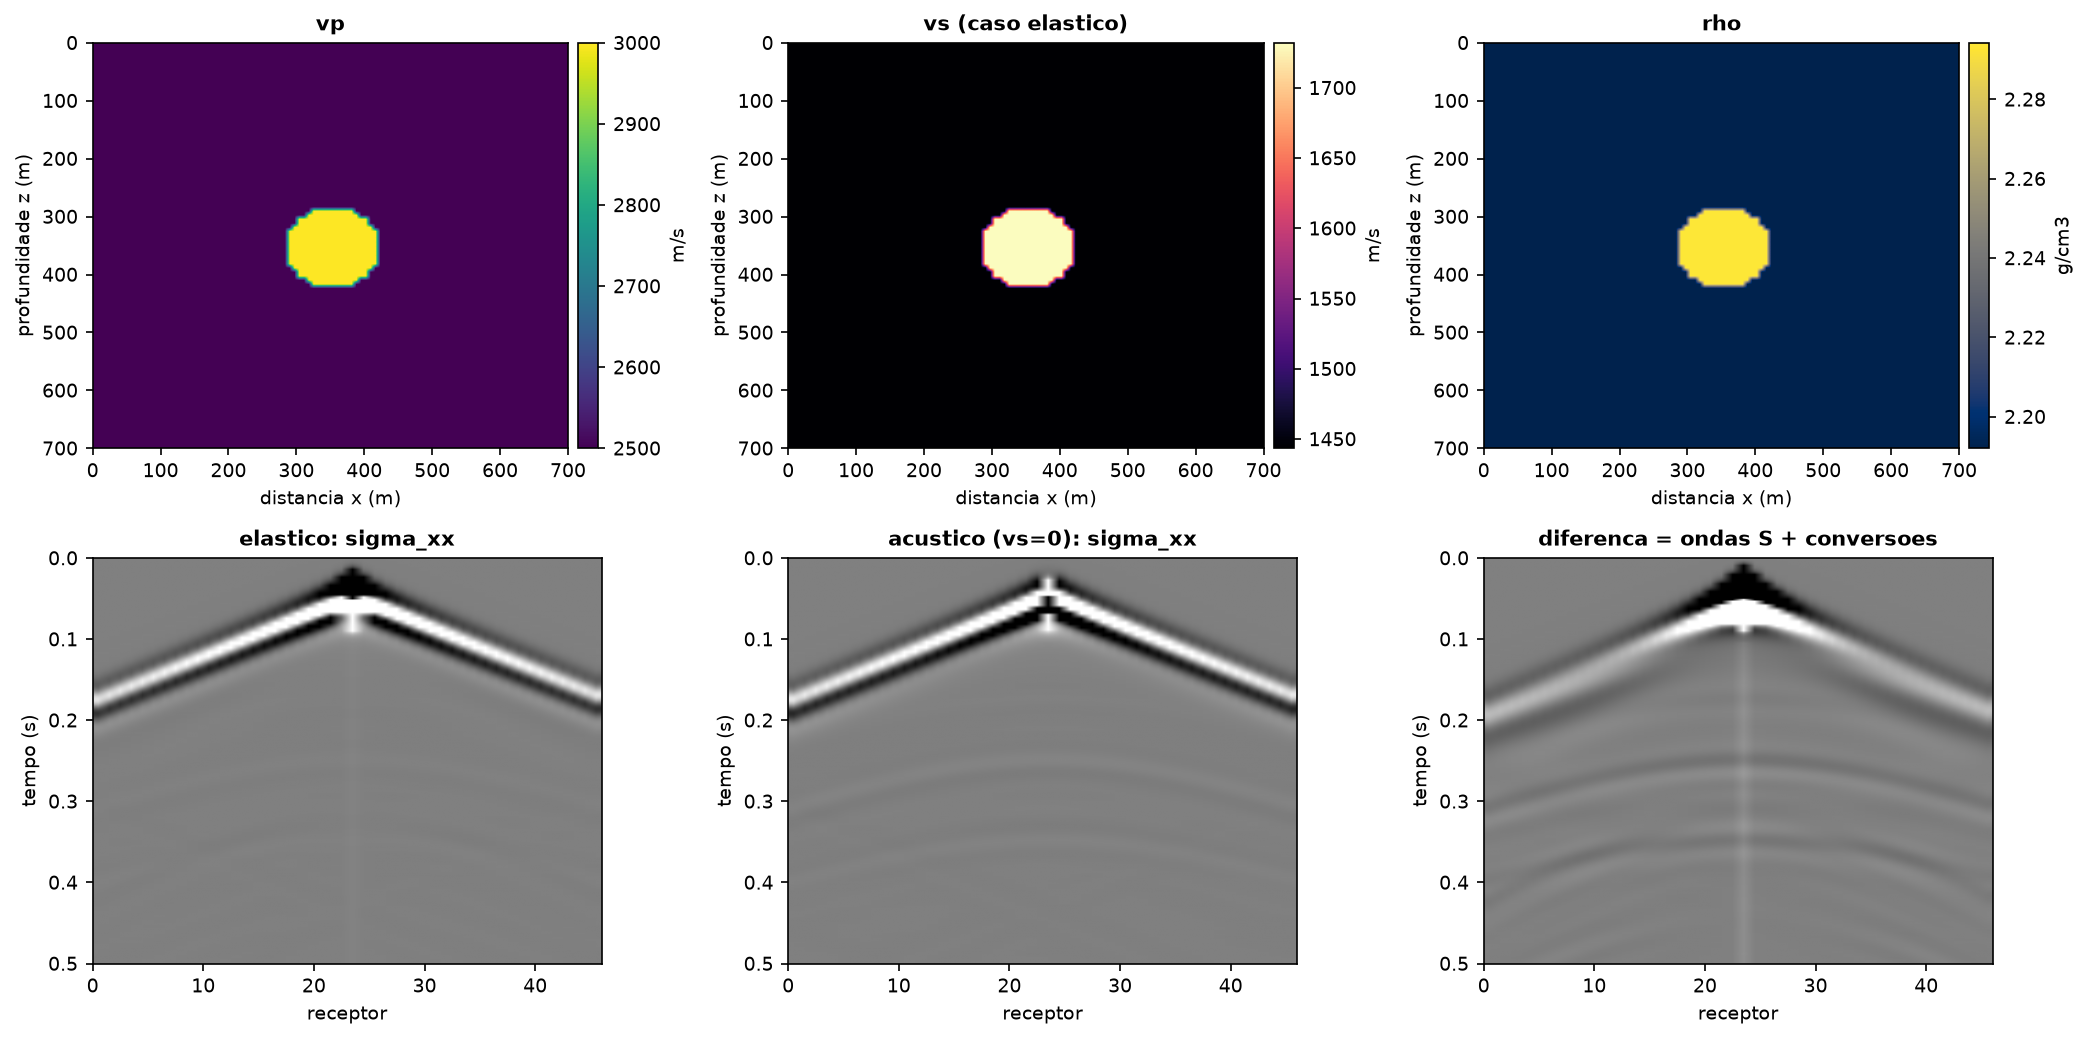
\includegraphics[width=0.96\textwidth]{../saidas/aula05/01_prova_regime_acustico.png}
\caption{Verifica\c{c}\~ao num\'erica de \eqref{eq:hipotese} em um solver
el\'astico de produ\c{c}\~ao: a mesma simula\c{c}\~ao com $v_s = v_p/\sqrt{3}$
e com $v_s = 0$. No caso ac\'ustico, $\norm{\sigma_{xx}-\sigma_{zz}}/
\norm{\sigma_{xx}}$ cai para $4{,}5\times10^{-7}$ (zero em \texttt{float32}) e
$\sigma_{xz}$ d\'a exatamente $0$. O painel inferior direito mostra a
diferen\c{c}a entre el\'astico e ac\'ustico --- ondas S e convers\~oes P--S,
com norma compar\'avel \`a do pr\'oprio dado.}
\end{figure}

\begin{matematica}[a transformada de Fourier, em meia p\'agina]
Qualquer sinal de energia finita pode ser escrito como soma de senoides:
\[
W(f) = \int_{-\infty}^{\infty} w(t)\,e^{-2\pi \mathrm{i} f t}\dd t ,
\qquad
w(t) = \int_{-\infty}^{\infty} W(f)\,e^{+2\pi \mathrm{i} f t}\dd f .
\]
$\abs{W(f)}$ \'e quanta energia h\'a na frequ\^encia $f$ --- o
\textbf{espectro de amplitude}; o argumento de $W(f)$ \'e a \textbf{fase}.

Quatro propriedades bastam para tudo o que se faz nesta cole\c{c}\~ao:
\begin{enumerate}[leftmargin=*, itemsep=1pt]
\item \textbf{Derivar no tempo $=$ multiplicar por $\mathrm{i}\omega$}
($\omega = 2\pi f$). Da\'i sai o espectro da Ricker, logo abaixo --- e da\'i
tamb\'em a armadilha da fonte da p\'agina anterior: uma derivada temporal a
mais \'e uma multiplica\c{c}\~ao por $\mathrm{i}\omega$, que muda a forma do
pulso sem mudar a f\'isica.
\item \textbf{Deslocar no tempo $=$ girar a fase}: $w(t-t_0)$ tem espectro
$W(f)e^{-2\pi\mathrm{i}ft_0}$, com a \emph{mesma} amplitude. \'E por isso que
um erro de tempo de tr\^ansito \'e um erro puramente de \textbf{fase} --- o
mecanismo do \emph{cycle skipping} (Cap.~\ref{cap:misfit}).
\item \textbf{Rela\c{c}\~ao rec\'iproca}: pulso estreito no tempo
$\Leftrightarrow$ espectro largo. N\~ao existe pulso curto e de banda estreita.
\item \textbf{Convolu\c{c}\~ao vira produto}: filtrar um tra\c{c}o \'e
multiplicar o espectro dele pelo do filtro --- \'e o que a multiescala faz a
cada banda.
\end{enumerate}
\end{matematica}

\section{A fonte: ondaleta de Ricker}
\label{sec:ricker}

Em trabalho sint\'etico usa-se quase sempre a Ricker, a segunda derivada de
uma gaussiana:
\begin{equation}
w(t) = \left[1 - 2\bigl(\pi f_0 (t-t_0)\bigr)^{2}\right]
       \exp\left[-\bigl(\pi f_0 (t-t_0)\bigr)^{2}\right].
\label{eq:ricker}
\end{equation}

\begin{derivacao}[O espectro, e de onde vem a banda]
Com $a = (\pi f_0)^{2}$, \eqref{eq:ricker} \'e
$w(t) = -\frac{1}{2a}\frac{\dd^{2}}{\dd t^{2}} e^{-a t^{2}}$. Como
$\mathcal{F}\{e^{-at^{2}}\} = \sqrt{\pi/a}\;e^{-\omega^{2}/4a}$ e a derivada
segunda vira $(i\omega)^{2} = -\omega^{2}$,
\begin{equation}
\abs{W(f)} = \frac{2}{\sqrt{\pi}}\,\frac{f^{2}}{f_0^{3}}\,
             e^{-f^{2}/f_0^{2}} .
\label{eq:ricker_espectro}
\end{equation}

O m\'aximo de \eqref{eq:ricker_espectro} est\'a em $f = f_0$: da\'i o nome
frequ\^encia de \textbf{pico}. Normalizando e resolvendo
$\abs{W(f)}/\abs{W(f_0)} = \eta$ com $u = (f/f_0)^{2}$, chega-se a
$u\,e^{1-u} = \eta$, cujas ra\'izes $u>1$ d\~ao
\[
\eta = 0{,}5\ (-6\,\text{dB}):\ f \approx 1{,}64 f_0,
\qquad
\eta = 0{,}1\ (-20\,\text{dB}):\ f \approx 2{,}21 f_0 .
\]
\end{derivacao}

Medindo numericamente no c\'odigo do curso, a banda confirma a conta:

\begin{center}
\begin{tabular}{@{}rrrrr@{}}
\toprule
$f_0$ (Hz) & pico medido & $f$ a $-6$\,dB & $/f_0$ & $/f_0$ a $-20$\,dB \\
\midrule
5  & 4{,}9  & 8{,}1  & 1{,}61 & 2{,}20 \\
10 & 10{,}0 & 16{,}1 & 1{,}61 & 2{,}20 \\
15 & 14{,}9 & 24{,}4 & 1{,}63 & 2{,}20 \\
25 & 24{,}9 & 40{,}8 & 1{,}63 & 2{,}21 \\
40 & 40{,}0 & 65{,}2 & 1{,}63 & 2{,}21 \\
\bottomrule
\end{tabular}
\end{center}

\begin{atencao}[Duas bandas, dois usos --- n\~ao confunda]
A banda a $\mathbf{-6}$\,\textbf{dB} ($\approx 1{,}6 f_0$) \'e a faixa que
\emph{move a invers\~ao}: use-a para raciocinar sobre \textbf{resolu\c{c}\~ao}.

A banda a $\mathbf{-20}$\,\textbf{dB} ($\approx 2{,}2 f_0$) ainda tem energia
suficiente para \emph{dispersar numericamente}: use-a para dimensionar a
\textbf{malha}, arredondando para $2{,}5 f_0$ por seguran\c{c}a.
\begin{equation}
\lambda_{\min} = \frac{c_{\min}}{f_{\max}}
 \ \ (\text{malha}: f_{\max} = 2{,}5 f_0),
\qquad
\delta_{\min} \approx \frac{\lambda}{2}
 \ \ (\text{resolu\c{c}\~ao}: f \approx 1{,}6 f_0).
\end{equation}
\end{atencao}

\subsection*{O atraso $t_0$}

A Ricker \eqref{eq:ricker} \'e n\~ao causal: tem energia em $t < t_0$. O
atraso padr\~ao $t_0 = 1/f_0$ n\~ao \'e arbitr\'ario --- \'e onde a amplitude
truncada em $t<0$ cai abaixo de $0{,}1\%$ do pico. Com
$t_0 = 0{,}6/f_0$ sobra $17{,}5\%$; com $0{,}8/f_0$, $2{,}1\%$; com
$1{,}0/f_0$, $0{,}10\%$. Truncar cedo demais injeta um degrau na fonte --- e
um degrau tem espectro largo, que dispersa.

\begin{exercicio}
\begin{enumerate}[leftmargin=*, itemsep=2pt]
\item Mostre, a partir de \eqref{eq:vpvs}, que o limite $\mu\to 0$ d\'a
$v_p \to \sqrt{K/\rho}$.
\item Um c\'odigo em press\~ao e outro em velocidade--tens\~ao, alimentados
com a mesma Ricker, produzem tra\c{c}os com correla\c{c}\~ao $+0{,}12$. Antes
de suspeitar da f\'isica, que tr\^es perguntas voc\^e faz?
\item Para $f_0 = 15$\,Hz, qual $f_{\max}$ voc\^e usaria para dimensionar a
malha, e qual para estimar a resolu\c{c}\~ao?
\end{enumerate}
\textbf{Respostas.} (1) Com $\mu = 0$, $\lambda = K$ e
$v_p = \sqrt{(\lambda+2\mu)/\rho} = \sqrt{K/\rho}$. (2) A formula\c{c}\~ao \'e
de primeira ou segunda ordem? A fonte entra na press\~ao, na tens\~ao ou na
velocidade de part\'icula? H\'a divis\~ao por $\Delta h^{2}$ na
discretiza\c{c}\~ao da delta? Cada escolha muda a ondaleta efetiva, e nenhuma
vem etiquetada no sismograma. (3) Malha: $2{,}5\times15 = 37{,}5$\,Hz;
resolu\c{c}\~ao: $1{,}6\times15 = 24$\,Hz.
\end{exercicio}

% =====================================================================
\chapter{Diferen\c{c}as finitas: estabilidade e dispers\~ao}
\label{cap:numerico}

\begin{ideia}
Duas restri\c{c}\~oes independentes governam a discretiza\c{c}\~ao. A
\textbf{estabilidade} decide se a simula\c{c}\~ao roda; a \textbf{dispers\~ao}
decide se ela est\'a certa. Cada uma tem uma f\'ormula fechada, e as duas
juntas determinam $\Delta h$ e $\Delta t$ sem nenhum chute.
\end{ideia}

\begin{matematica}[s\'erie de Taylor e a ideia de ``ordem'']
Toda a discretiza\c{c}\~ao deste cap\'itulo sai de uma \'unica ferramenta. Se
$f$ \'e suave,
\[
f(x+h) = f(x) + h f'(x) + \frac{h^{2}}{2}f''(x) + \frac{h^{3}}{6}f'''(x)
 + \dots
\]
--- o valor num ponto vizinho \'e o valor aqui, mais corre\c{c}\~oes que
encolhem como pot\^encias de $h$.

\textbf{Ordem de aproxima\c{c}\~ao.} Dizer que um esquema \'e
$\mathcal{O}(h^{n})$ significa que o erro cai como $h^{n}$: reduzir $h$ pela
metade divide o erro por $2^{n}$. \'E uma afirma\c{c}\~ao sobre a
\emph{taxa}, n\~ao sobre o \emph{valor} --- um esquema de ordem 8 pode ser
pior que um de ordem 2 para $h$ grande, e \'e imbat\'ivel para $h$ pequeno.

\textbf{Como se mede na pr\'atica.} Rode com $h$ e com $h/2$ e calcule
$\log_2(\text{erro}_h/\text{erro}_{h/2})$: esse n\'umero deve dar $n$. \'E
\emph{exatamente} o mesmo procedimento que o teste de Taylor do
Cap\'itulo~\ref{cap:verificacao} usa para validar o gradiente, com $\alpha$
no lugar de $h$.

\textbf{Por que est\^enceis centrados t\^em ordem par.} Somando $f(x+h)$ com
$f(x-h)$, todos os termos de pot\^encia \emph{\'impar} se cancelam. O erro
come\c{c}a em $h^{2}$ --- de gra\c{c}a, s\'o pela simetria.
\end{matematica}

\section{O operador espacial e seus coeficientes}
\label{sec:taylor-fd}

A derivada segunda \'e aproximada por um est\^encil centrado de $2N+1$ pontos:
\begin{equation}
\frac{\partial^{2} f}{\partial x^{2}}\bigg|_{i} \approx
\frac{1}{h^{2}}\left[c_0 f_i + \sum_{j=1}^{N} c_j\,(f_{i+j} + f_{i-j})\right].
\label{eq:estencil}
\end{equation}

\begin{derivacao}[De onde saem os coeficientes]
Expanda $f_{i\pm j} = f(x_i \pm jh)$ em s\'erie de Taylor e some os pares:
\[
f_{i+j} + f_{i-j}
 = 2\sum_{\ell=0}^{\infty} \frac{(jh)^{2\ell}}{(2\ell)!}\, f^{(2\ell)}_i
 = 2f_i + (jh)^2 f''_i + \frac{(jh)^4}{12}f^{(4)}_i + \dots
\]
(os termos \'impares se cancelam, que \'e a raz\~ao de o est\^encil centrado
ter ordem par). Substituindo em \eqref{eq:estencil} e exigindo que o resultado
reproduza $f''_i$ com erro $\mathcal{O}(h^{2N})$, obt\^em-se as
\textbf{condi\c{c}\~oes de momento}:
\begin{equation}
c_0 + 2\sum_{j=1}^{N} c_j = 0,
\qquad
2\sum_{j=1}^{N} j^{2} c_j = 2,
\qquad
\sum_{j=1}^{N} j^{2\ell} c_j = 0 \quad (\ell = 2,\dots,N).
\end{equation}
S\~ao $N+1$ equa\c{c}\~oes lineares em $N+1$ inc\'ognitas --- sistema de
Vandermonde, sempre sol\'uvel. A primeira condi\c{c}\~ao diz que o est\^encil
anula constantes; a segunda o normaliza; as demais matam os termos de erro
sucessivos.
\end{derivacao}

\begin{center}
\begin{tabular}{@{}llp{7.4cm}@{}}
\toprule
\textbf{Ordem} & \textbf{Pontos} & \textbf{Coeficientes $(c_0, c_1, \dots)$} \\
\midrule
$\mathcal{O}(h^{2})$ & 3 & $-2$; $+1$ \\
$\mathcal{O}(h^{4})$ & 5 & $-5/2$; $+4/3$; $-1/12$ \\
$\mathcal{O}(h^{8})$ & 9 & $-205/72$; $+8/5$; $-1/5$; $+8/315$; $-1/560$ \\
\bottomrule
\end{tabular}
\end{center}

Verifica\c{c}\~ao num\'erica em $f(x) = \sin(kx)$, com o \emph{mesmo} $h$: o
erro relativo medido pelo c\'odigo do curso \'e $7{,}5\times10^{-3}$ na ordem
2, $8{,}9\times10^{-5}$ na ordem 4 e $2{,}0\times10^{-8}$ na ordem 8 --- cinco
ordens de grandeza entre os extremos.

\begin{atencao}[Ordem alta n\~ao \'e luxo: \'e economia --- e a conta completa]
O ganho n\~ao \'e ``mais preciso'', \'e \textbf{mais preciso para o mesmo
$h$}, e portanto permite $h$ \emph{maior}. Para um \emph{mesmo} esquema, o
custo em 2D escala com $h^{-3}$ --- dois eixos espaciais e, via CFL, o eixo do
tempo.

Ao \emph{trocar} de esquema, por\'em, tr\^es fatores mudam ao mesmo tempo, e
vale fechar a conta com todos. Trocando $\mathcal{O}(2)$ por
$\mathcal{O}(8)$, a exig\^encia de $G$ cai de $\sim$15--20 para $\sim$4--5,
o que permite $\Delta h$ cerca de $3\times$ maior:

\begin{center}
\begin{tabular}{@{}lrl@{}}
\toprule
\textbf{Fator} & \textbf{Efeito} & \textbf{Origem} \\
\midrule
pontos da malha & $\div\,9$ & $\Delta h$ $3\times$ maior, em 2D \\
passos de tempo & $\div\,2{,}4$ & $\Delta t \propto C_{\lim}\Delta h$, com
  $C_{\lim}$ caindo de $0{,}71$ a $0{,}55$ \\
opera\c{c}\~oes por ponto & $\times\,3{,}4$ & est\^encil de 17 pontos em vez
  de 5 \\
\midrule
\textbf{saldo} & $\mathbf{\div\,6}$ & \\
\bottomrule
\end{tabular}
\end{center}

Ou seja: a ordem alta compensa, e por uma margem grande --- mas o fator n\~ao
\'e o $h^{-3}$ ing\^enuo. Se $\Delta h$ fosse apenas dobrado em vez de
triplicado, o saldo cairia para cerca de $\div\,1{,}8$.
\end{atencao}

\begin{matematica}[modos de Fourier na malha e o fator de amplifica\c{c}\~ao]
A an\'alise de estabilidade a seguir usa um truque que vale entender uma vez e
reconhecer para sempre.

\textbf{A ideia.} O esquema \'e linear e, em meio homog\^eneo, tem
coeficientes constantes. Ent\~ao ele \emph{n\~ao mistura} modos de Fourier: se
voc\^e o alimentar com uma \'unica onda plana
$p_i^{n} = \xi^{n}e^{\mathrm{i}\mathbf{k}\cdot\mathbf{x}_i}$, ela continua
sendo uma \'unica onda plana ap\'os um passo, apenas multiplicada por um
n\'umero $\xi$ --- o \textbf{fator de amplifica\c{c}\~ao}.

\textbf{O crit\'erio.} Ap\'os $n$ passos, a amplitude vale $\xi^{n}$. Logo:
\[
\abs{\xi} \le 1 \ \text{para todo } \mathbf{k}
\ \Longrightarrow\ \text{est\'avel};
\qquad
\abs{\xi} > 1 \ \text{para algum } \mathbf{k}
\ \Longrightarrow\ \text{cresce exponencialmente}.
\]
Como basta \emph{um} modo inst\'avel para arruinar tudo, a condi\c{c}\~ao \'e
sempre um \emph{pior caso} sobre $\mathbf{k}$ --- e o pior caso \'e o modo
mais curto que a malha representa, de comprimento de onda $2\Delta h$, isto
\'e $k\Delta h = \pi$.

\textbf{A conta que aparece a seguir.} A discretiza\c{c}\~ao de
$\partial_{tt}$ produz uma equa\c{c}\~ao do segundo grau
$\xi^{2}-(2-X)\xi+1=0$. Como o produto das ra\'izes vale 1, ou as duas t\^em
m\'odulo 1 (ra\'izes complexas: o modo \emph{oscila}, que \'e o que uma onda
deve fazer), ou uma tem m\'odulo maior que 1 (ra\'izes reais: o modo
\emph{cresce}). A fronteira entre os dois casos \'e o discriminante zero --- e
\'e ela que d\'a a condi\c{c}\~ao CFL.

\textbf{Dispers\~ao, com a mesma ferramenta.} Trocando
$\xi = e^{-\mathrm{i}\omega\Delta t}$ --- isto \'e, exigindo que o modo oscile
com frequ\^encia $\omega$ ---, a mesma equa\c{c}\~ao passa a relacionar
$\omega$ com $k$: \'e a \emph{rela\c{c}\~ao de dispers\~ao}. Estabilidade e
dispers\~ao saem da mesma conta, feita duas vezes com perguntas diferentes.
\end{matematica}

\section{Estabilidade: a condi\c{c}\~ao CFL}

No tempo usa-se o esquema \emph{leap-frog} de segunda ordem:
\begin{equation}
p_i^{n+1} = 2p_i^{n} - p_i^{n-1}
 + c_i^{2}\,\Delta t^{2}\left(\left[\nabla^{2}_{h} p^{n}\right]_i
 + s_i^{n}\right).
\label{eq:leapfrog}
\end{equation}

\begin{derivacao}[An\'alise de von Neumann]
Procure solu\c{c}\~oes da forma $p_i^{n} = \xi^{n} e^{\mathrm{i}\mathbf{k}
\cdot\mathbf{x}_i}$ em meio homog\^eneo, sem fonte. O operador
\eqref{eq:estencil} aplicado a $e^{\mathrm{i}kx}$ devolve
\begin{equation}
\frac{1}{h^{2}}\Bigl[c_0 + 2\sum_{j} c_j\cos(j\,k_x h)\Bigr]
 \;=\; -\frac{S(k_x h)}{h^{2}},
\qquad
S(\theta) \equiv -\Bigl[c_0 + 2\sum_{j} c_j\cos(j\theta)\Bigr] \ge 0 .
\end{equation}
Substituindo em \eqref{eq:leapfrog} e escrevendo $\xi + \xi^{-1} = 2 - X$, com
\[
X = \frac{c^{2}\Delta t^{2}}{\Delta h^{2}}
    \bigl[S(k_x\Delta h) + S(k_z\Delta h)\bigr],
\]
obt\'em-se $\xi^{2} - (2-X)\xi + 1 = 0$. As ra\'izes t\^em produto 1, logo
$\abs{\xi} = 1$ (n\~ao amplifica) \textbf{se e somente se} as ra\'izes forem
complexas conjugadas, o que exige $\abs{2 - X} \le 2$, isto \'e
$0 \le X \le 4$. Se $X > 4$, uma raiz tem m\'odulo $> 1$ e o esquema
\emph{amplifica exponencialmente}.

(O \'indice $j$ percorre o est\^encil; n\~ao confundir com o n\'umero de onda
$k_x$, que entra apenas atrav\'es de $\theta = k_x h$.)

O pior caso \'e $\theta = \pi$ em cada eixo --- o modo mais curto que a malha
representa ---, onde $S(\pi) = \abs{c_0} + 2\sum_j\abs{c_j}$ para os
est\^enceis desta tabela. Com $n_{\dim}$ dimens\~oes:
\end{derivacao}

\begin{equation}
\boxed{\;
C \equiv \frac{c_{\max}\,\Delta t}{\Delta h} \;\le\; C_{\lim}
 = \frac{2}{\sqrt{n_{\dim}\bigl(\abs{c_0} + 2\sum_j \abs{c_j}\bigr)}}\;}
\label{eq:cfl}
\end{equation}

\begin{center}
\begin{tabular}{@{}lrrr@{}}
\toprule
\textbf{Ordem espacial} & $\abs{c_0}+2\sum_j\abs{c_j}$ & $C_{\lim}$ (2D)
& $C_{\lim}$ (3D) \\
\midrule
$\mathcal{O}(2)$ & $4{,}000$ & $0{,}7071$ & $0{,}5774$ \\
$\mathcal{O}(4)$ & $5{,}333$ & $0{,}6124$ & $0{,}5000$ \\
$\mathcal{O}(8)$ & $6{,}502$ & $0{,}5546$ & $0{,}4529$ \\
\bottomrule
\end{tabular}
\end{center}

\begin{atencao}[Duas leituras contraintuitivas]
\textbf{(a) Ordem espacial maior \emph{reduz} $\Delta t_{\max}$.} O est\^encil
mais largo tem $S(\pi)$ maior, e \eqref{eq:cfl} aperta. Ganha-se em $\Delta h$
e perde-se em $\Delta t$ --- com saldo favor\'avel, mas a conta precisa ser
feita.

\textbf{(b) O limite depende de $c_{\max}$, n\~ao de $c$ t\'ipico.} Uma
\'unica c\'elula r\'apida --- sal, basalto, um artefato de interpola\c{c}\~ao
--- derruba $\Delta t$ do modelo inteiro. Vale inspecionar
$\max(c)$ antes de rodar.
\end{atencao}

A transi\c{c}\~ao n\~ao \'e gradual: com $C_{\lim} = 0{,}6124$, o curso mediu
$C = 0{,}306$ e $C = 0{,}551$ est\'aveis, e $C = 0{,}625$ e $C = 0{,}704$
produzindo \texttt{NaN}. Use margem de 10--20\%.

\section{Dispers\~ao num\'erica}

Estabilidade garante que a solu\c{c}\~ao n\~ao explode; n\~ao garante que ela
esteja certa. No esquema discreto, a velocidade de fase depende do n\'umero de
onda: as componentes curtas viajam com velocidade errada e o pulso desenvolve
uma cauda oscilat\'oria.

\begin{derivacao}[A rela\c{c}\~ao de dispers\~ao completa]
Repetindo a an\'alise de von Neumann com $\xi = e^{-\mathrm{i}\omega\Delta t}$
(solu\c{c}\~ao propagante), $\xi + \xi^{-1} = 2\cos(\omega\Delta t)$, e usando
$2 - 2\cos\theta = 4\sin^{2}(\theta/2)$:
\begin{equation}
\boxed{\;
\frac{4}{\Delta t^{2}}\sin^{2}\!\left(\frac{\omega\Delta t}{2}\right)
 = \frac{c^{2}}{\Delta h^{2}}\,
   \bigl[S(k_x\Delta h) + S(k_z\Delta h)\bigr] \;}
\label{eq:dispersao}
\end{equation}
A velocidade de fase num\'erica \'e $c_{\text{num}} = \omega/k$, e a grandeza
diagn\'ostica \'e a raz\~ao $c_{\text{num}}/c$, que deveria valer 1.

Tomando $\Delta t \to 0$ em \eqref{eq:dispersao} recupera-se a curva
\emph{semi-discreta} (s\'o o erro espacial), que \'e a curva mostrada na
maioria dos livros.
\end{derivacao}

O controle pr\'atico \'e o n\'umero de pontos por comprimento de onda:
\begin{equation}
G = \frac{\lambda_{\min}}{\Delta h} = \frac{c_{\min}}{f_{\max}\,\Delta h},
\qquad
G \gtrsim
\begin{cases}
15\text{--}20 & \mathcal{O}(2)\\
8\text{--}10  & \mathcal{O}(4)\\
4\text{--}5   & \mathcal{O}(8)
\end{cases}
\label{eq:G}
\end{equation}

\begin{armadilha}[A curva espacial \emph{n\~ao} \'e conservadora]
Este ponto quase nunca aparece, e inverte a conclus\~ao usual.

A discretiza\c{c}\~ao temporal acrescenta um erro pr\'oprio de sinal
\textbf{oposto}: o est\^encil espacial \emph{atrasa} a fase, o \emph{leap-frog}
a \emph{adianta}. O quanto um compensa o outro depende de $C$.

Medidas do curso, para $\mathcal{O}(4)$ com $G=6$: a curva espacial prev\^e
$c_{\text{num}}/c = 0{,}9939$ (erro de $0{,}6\%$). O esquema completo
\eqref{eq:dispersao} d\'a $0{,}9980$ com $C=0{,}3$ --- \emph{melhor} que o
previsto --- mas $1{,}0081$ com $C=0{,}551$: erro real de $0{,}8\%$, j\'a
\textbf{maior} que o previsto pela curva.

Em $\mathcal{O}(8)$ o efeito \'e dram\'atico: com $G=5$ e
$C = 0{,}9\,C_{\lim} \approx 0{,}50$ a curva espacial promete $0{,}07\%$ e o
esquema completo entrega $1{,}6\%$ --- porque
o erro espacial praticamente sumiu e sobrou o temporal, sozinho.

\textbf{Conclus\~ao:} perto do limite CFL, e sobretudo em ordem alta, quem
dita a dispers\~ao \'e $\Delta t$. Dimensione por \eqref{eq:dispersao}, n\~ao
pela curva espacial.
\end{armadilha}

\begin{figure}[htbp]
\centering
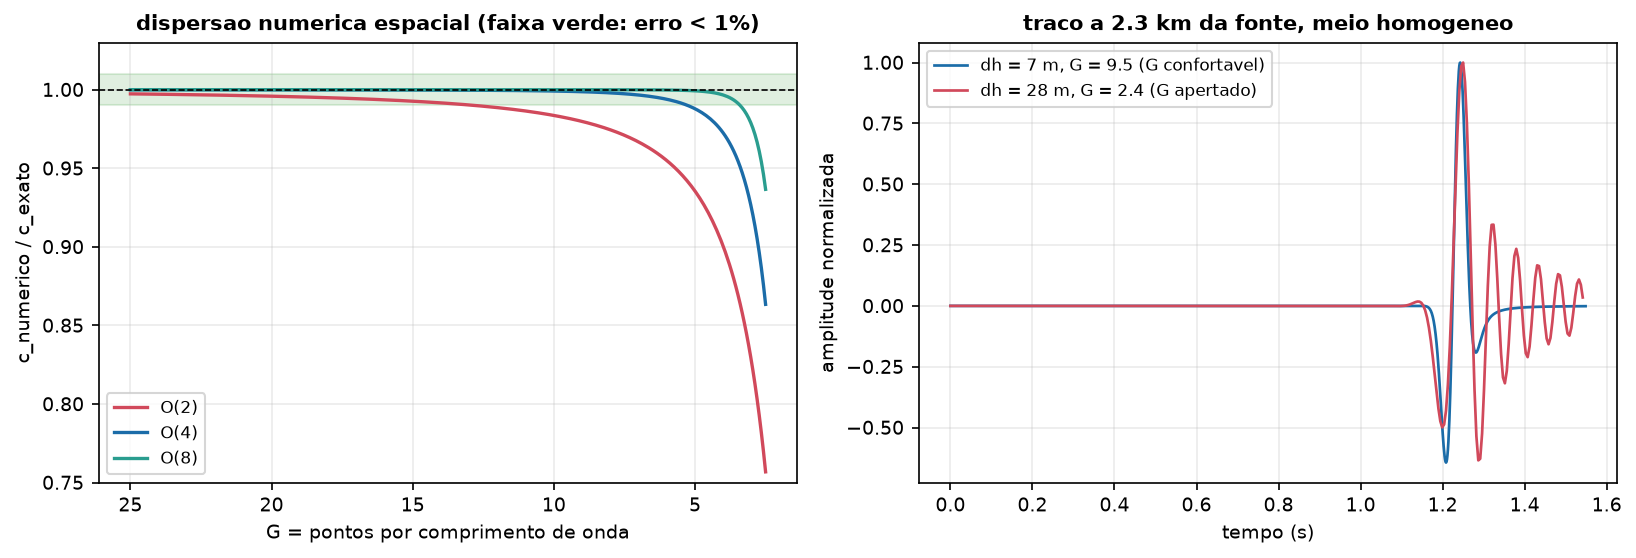
\includegraphics[width=0.96\textwidth]{../saidas/aula02/01_dispersao_numerica.png}
\caption{Esquerda: dispers\~ao do operador espacial isolado, por ordem.
Direita: tra\c{c}o a 2{,}3\,km da fonte em meio homog\^eneo, com $G=9{,}5$ e
$G=2{,}4$. A cauda do tra\c{c}o vermelho n\~ao existe na f\'isica --- e
\emph{parece} geologia.}
\end{figure}

\begin{pratica}[O teste de cinco minutos]
Num meio \textbf{homog\^eneo} n\~ao h\'a o que refletir. Qualquer
oscila\c{c}\~ao depois do primeiro pulso \'e erro num\'erico. Rode esse teste
antes de qualquer invers\~ao: \'e o \'unico jeito barato de separar artefato
de sinal.
\end{pratica}

\section{Receita de dimensionamento}

\begin{lstlisting}
1. f_max  = 2.5 * f0                    # banda conservadora da Ricker
2. dh     = c_min / (G * f_max)         # G = 8 (O4) ou 5 (O8)
3. dt     = 0.9 * C_lim * dh / c_max    # margem de 10% (O8: reduza C)
4. nt     = tempo_de_registro / dt
5. n_abs >= 0.5 * c_max / (f_min * dh)  # moldura -- Capitulo 4
\end{lstlisting}

\begin{atencao}[O conflito embutido]
$\Delta h$ \'e ditado por $c_{\min}$ (menor comprimento de onda) e $\Delta t$
por $c_{\max}$ (onda mais r\'apida). Um modelo com grande contraste --- \'agua
a 1500 e sal a 4500 --- \'e caro dos \emph{dois} lados simultaneamente. \'E a
raz\~ao pr\'atica de existirem malhas de espa\c{c}amento vari\'avel e esquemas
impl\'icitos.
\end{atencao}

\textbf{Escalonamento do custo:} reduzir $\Delta h$ pela metade quadruplica o
n\'umero de pontos em 2D \emph{e} dobra o n\'umero de passos (via CFL):
$8\times$ em 2D, $16\times$ em 3D.

\begin{exercicio}
\begin{enumerate}[leftmargin=*, itemsep=2pt]
\item Verifique que o est\^encil $\mathcal{O}(4)$ satisfaz as tr\^es
condi\c{c}\~oes de momento.
\item Modelo com $c \in [1500, 4500]$\,m/s, $f_0 = 10$\,Hz, ordem 8, 2D.
Calcule $\Delta h$, $\Delta t$ e o n\'umero de passos para 4\,s de registro.
\item A sua simula\c{c}\~ao em ordem 8 com $G = 5$ mostra mais dispers\~ao que
a curva prometia. Qual \'e a primeira suspeita, e qual o conserto mais barato?
\end{enumerate}
\textbf{Respostas.} (1) $c_0 + 2(c_1+c_2) = -5/2 + 2(4/3 - 1/12) = -5/2 + 5/2
= 0$; $2(1^2 c_1 + 2^2 c_2) = 2(4/3 - 4/12) = 2$; $1^4 c_1 + 2^4 c_2 =
4/3 - 16/12 = 0$. (2) $f_{\max}=25$\,Hz; $\lambda_{\min}=60$\,m;
$\Delta h = 60/5 = 12$\,m; $\Delta t = 0{,}9\times0{,}5546\times12/4500
\approx 1{,}33$\,ms; $n_t \approx 3000$. (3) O erro temporal dominando ---
veja a caixa acima. O conserto mais barato \'e reduzir $C$ (usar $\Delta t$
menor), n\~ao refinar a malha.
\end{exercicio}

% =====================================================================
\chapter{Bordas, superf\'icie livre e aquisi\c{c}\~ao}
\label{cap:bordas}

\begin{ideia}
O dom\'inio truncado reflete; a moldura absorvente existe para apagar esse
eco. O topo \'e diferente: ali h\'a uma interface real, e o que se escolhe
n\~ao \'e num\'erico, \'e f\'isico. E a geometria de aquisi\c{c}\~ao define,
antes de qualquer algoritmo, o que ser\'a poss\'ivel recuperar.
\end{ideia}

\section{Por que as bordas n\~ao s\~ao detalhe}

Truncar o dom\'inio transforma a borda num espelho. Em modelagem isso \'e
feio; em FWI \'e pior: o res\'iduo passa a conter eventos que a f\'isica do
modelo nunca vai explicar, e o gradiente tenta explic\'a-los mexendo na
velocidade.

\begin{center}
\begin{tabular}{@{}lp{5.2cm}ll@{}}
\toprule
\textbf{T\'ecnica} & \textbf{Como} & \textbf{Custo} & \textbf{Qualidade} \\
\midrule
Truncar & nada & zero & inaceit\'avel \\
Cerjan (\emph{sponge}) & \emph{taper} multiplicativo na moldura & baixo
  & razo\'avel \\
Cond.\ absorvente & equa\c{c}\~ao unidirecional na face & baixo & boa em
  incid\^encia normal \\
CPML & coordenadas complexas esticadas & m\'edio & excelente \\
\bottomrule
\end{tabular}
\end{center}

\subsection*{Cerjan: a f\'ormula e o \'otimo}

O \emph{sponge} multiplica o campo, a cada passo, por um fator que decai para
dentro da moldura:
\begin{equation}
w(d) = \exp\!\left[-\bigl(\beta\, d\bigr)^{2}\right],
\qquad d = \text{dist\^ancia \`a borda do dom\'inio f\'isico},
\label{eq:cerjan}
\end{equation}
com $d$ contado em c\'elulas, de $0$ (in\'icio da moldura) a $n_{abs}$.

\begin{teoria}[Existe um \'otimo, e ele n\~ao \'e ``o mais forte poss\'ivel'']
\emph{Taper} fraco demais n\~ao absorve: a onda atravessa a moldura, bate na
parede e volta. \emph{Taper} forte demais cria um degrau de imped\^ancia na
\emph{entrada} da moldura, que ele mesmo reflete.

O \'otimo medido fica em $\beta \approx 0{,}25/n_{abs}$ --- ou seja, o
\emph{taper} deve ser dimensionado \textbf{em fun\c{c}\~ao da espessura}, e
n\~ao fixado. Um valor de $\beta$ calibrado para 20 c\'elulas fica fraco
demais em 45 e forte demais em 10.
\end{teoria}

\begin{pratica}[Por que este curso usa Cerjan mesmo sendo inferior]
O \emph{sponge} \'e um operador \textbf{diagonal}, portanto \textbf{auto-adjunto}.
Isso preserva a validade do teste de gradiente do
Cap\'itulo~\ref{cap:verificacao} sem exigir que voc\^e derive o adjunto de uma
CPML --- que \'e trabalhoso e uma fonte cl\'assica de erro silencioso.

Em produ\c{c}\~ao usa-se CPML e deriva-se o seu adjunto (ou aceita-se o erro
e documenta-se).
\end{pratica}

\subsection*{Medindo de verdade}

Para medir reflex\~ao de borda \'e preciso uma \textbf{refer\^encia sem
borda}: a mesma simula\c{c}\~ao num dom\'inio muito maior, onde nada reflete
dentro da janela de tempo. A diferen\c{c}a entre os dois tra\c{c}os \'e, por
constru\c{c}\~ao, s\'o artefato.

\begin{center}
\begin{tabular}{@{}rrrr@{}}
\toprule
\multicolumn{2}{c}{\textbf{Cerjan}} & \multicolumn{2}{c}{\textbf{CPML}} \\
$n_{abs}$ & reflex\~ao & $n_{pml}$ & reflex\~ao \\
\midrule
0  & $-6{,}9$ dB  & 0  & $-11{,}2$ dB \\
10 & $-8{,}5$ dB  & 5  & $-20{,}1$ dB \\
20 & $-13{,}3$ dB & 10 & $-51{,}5$ dB \\
30 & $-16{,}5$ dB & 20 & $-69{,}6$ dB \\
45 & $-18{,}4$ dB & 30 & $-77{,}3$ dB \\
\bottomrule
\end{tabular}
\end{center}

\begin{atencao}[Como comparar honestamente]
Os valores s\~ao relativos \`a onda direta de \emph{cada} experimento, e as
duas geometrias diferem. A linha $n=0$ \'e o espelho --- reflex\~ao de 100\%,
j\'a atenuada pelo espalhamento geom\'etrico --- e a compara\c{c}\~ao justa
desconta esse valor: o Cerjan com 45 pontos fica $11{,}5$\,dB abaixo do seu
espelho; a CPML com 10 pontos fica $40{,}3$\,dB abaixo do dela.

A conclus\~ao n\~ao muda, s\'o fica precisa: \textbf{CPML com 10 pontos supera
com folga Cerjan com 45}. \'E por isso que c\'odigos de produ\c{c}\~ao usam
CPML.
\end{atencao}

\textbf{Dimensionamento:} a moldura precisa de pelo menos meio comprimento de
onda da \emph{menor} frequ\^encia usada. Como a FWI multiescala come\c{c}a nas
bandas baixas, dimensione por $f_{\min}$ --- nunca por $f_0$.

\section{Superf\'icie livre}

No topo h\'a uma decis\~ao que n\~ao \'e num\'erica:

\textbf{Superf\'icie livre} ($p = 0$ em $z = 0$) representa a interface com o
ar. A onda reflete com polaridade invertida e produz as \emph{m\'ultiplas} de
superf\'icie e o \emph{ghost} --- eventos reais do dado.

\textbf{Borda absorvente no topo} representa um meio que continua para cima.
N\~ao \'e f\'isico, mas elimina m\'ultiplas do sint\'etico.

\begin{derivacao}[Implementar $p=0$ corretamente: o m\'etodo das imagens]
A tenta\c{c}\~ao \'e zerar as $N$ primeiras linhas da malha (o alcance do
est\^encil). Isso est\'a \textbf{errado}: p\~oe a superf\'icie efetiva em
$z = (N-1)\Delta h$, e n\~ao em $z = 0$ --- um erro de posicionamento que
desloca todas as m\'ultiplas.

O correto \'e a \textbf{imagem antissim\'etrica}: estender o campo para
$z < 0$ com
\begin{equation}
p(-z, t) = -p(z, t),
\end{equation}
o que imp\~oe $p = 0$ \emph{exatamente} em $z = 0$ por simetria, e alimenta o
est\^encil com valores consistentes. \'E assim que o propagador do curso faz.
\end{derivacao}

\begin{armadilha}[O erro de consist\^encia]
Se o dado observado cont\'em m\'ultiplas e o sint\'etico n\~ao, esse res\'iduo
inteiro vai para o gradiente, e a FWI tenta reproduzir as m\'ultiplas mexendo
na velocidade. As sa\'idas s\~ao duas: modelar a superf\'icie livre, ou
remover as m\'ultiplas do dado antes. Ignorar n\~ao \'e op\c{c}\~ao.
\end{armadilha}

\section{Aquisi\c{c}\~ao}
\label{sec:aquisicao}

A FWI trabalha em \emph{shot gathers}, e a raz\~ao \'e conceitual: $F$ simula
tiros, ent\~ao o res\'iduo $F(\mvec) - \dobs$ tem de ser calculado nessa
organiza\c{c}\~ao --- um tiro por vez ou, para acelerar, somas codificadas de
tiros que o simulador reproduz exatamente (Krebs \emph{et al.}, 2009; N\'ivel 3,
Cap.~8). O que ela n\~ao usa \'e o dado empilhado do processamento: o
empilhamento descarta a depend\^encia com o afastamento, que \'e justamente a
informa\c{c}\~ao que separa velocidade de profundidade.

\begin{figure}[htbp]
\centering
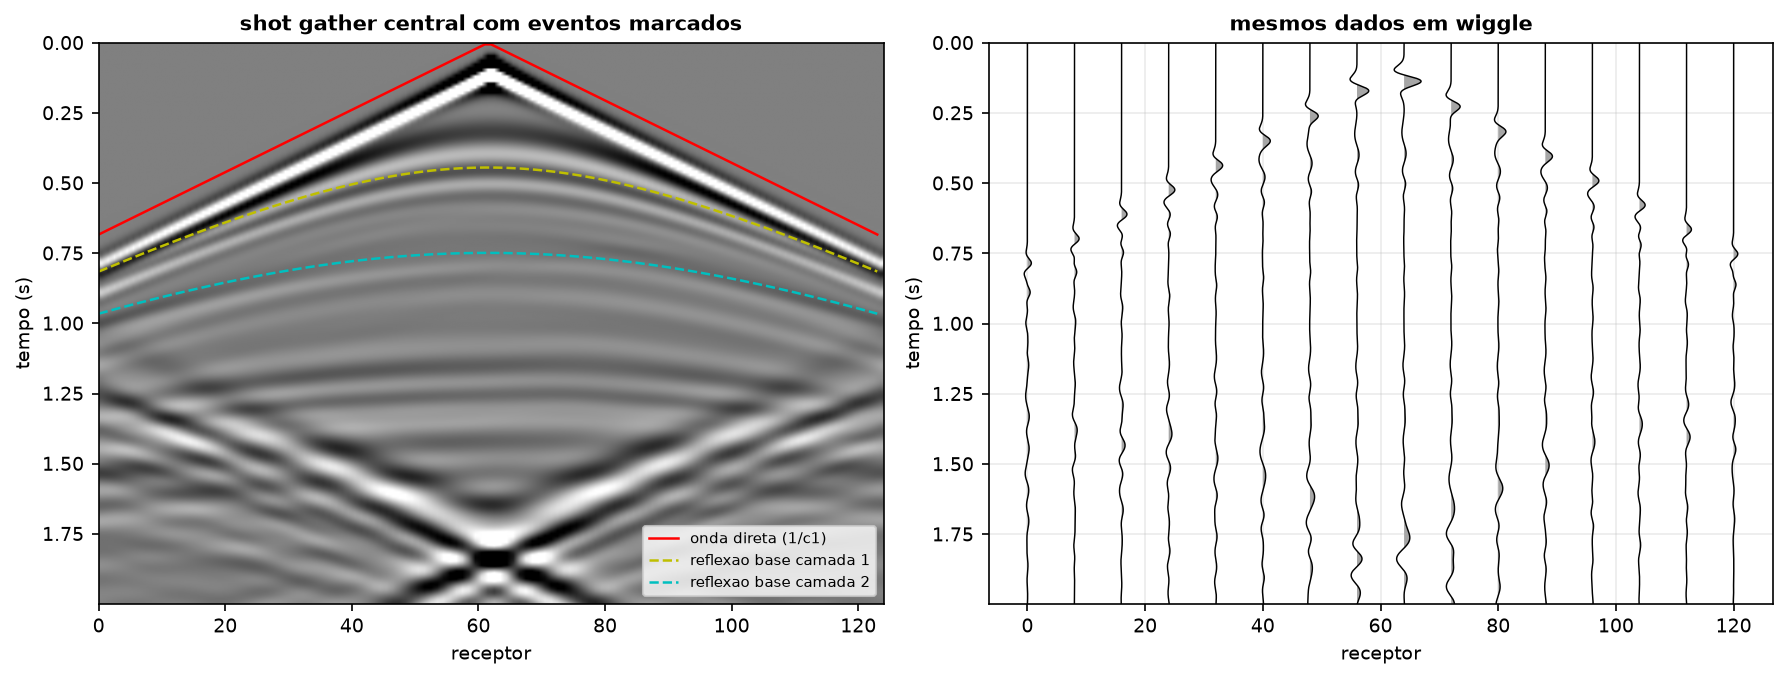
\includegraphics[width=0.95\textwidth]{../saidas/aula04/02_anatomia_shot_gather.png}
\caption{Anatomia de um \emph{shot gather} com as curvas te\'oricas
sobrepostas: onda direta (reta pela origem) e reflex\~oes (hip\'erboles).}
\end{figure}

\subsection*{Anatomia, com as f\'ormulas}

\begin{itemize}[leftmargin=*]
\item \textbf{Onda direta}: $t = x/c_1$ --- reta de inclina\c{c}\~ao $1/c_1$
passando pela origem. N\~ao carrega informa\c{c}\~ao de profundidade;
frequentemente \'e removida.
\item \textbf{Refra\c{c}\~oes} (\emph{head waves}): retas de inclina\c{c}\~ao
$1/c_2$. Dois n\'umeros diferentes as caracterizam, e confundi-los \'e comum:
\begin{align}
x_{\text{crit}} &= 2h_1\tan\theta_c, \qquad \sin\theta_c = c_1/c_2
  && \text{(onde ela come\c{c}a a existir)}\\[2pt]
x_{\text{cross}} &= 2h_1\sqrt{\frac{c_2+c_1}{c_2-c_1}}
  && \text{(onde ultrapassa a direta)}
\end{align}
A segunda \'e bem maior que a primeira --- no modelo da aula 04 do curso,
2291\,m contra 1006\,m. As refra\c{c}\~oes dominam o afastamento longo e s\~ao
a fonte mais rica de informa\c{c}\~ao sobre velocidade de grande escala.
\item \textbf{Reflex\~oes}: $t(x)^{2} \approx t_0^{2} + x^{2}/v_{\text{rms}}^{2}$
--- hip\'erboles cuja curvatura revela a velocidade RMS at\'e o refletor
(exata para uma camada; em meio estratificado, aproxima\c{c}\~ao de afastamento
pequeno).
\item \textbf{Difra\c{c}\~oes}: hip\'erboles de \'apice deslocado, geradas por
pontos isolados.
\end{itemize}

\begin{teoria}[Abertura e profundidade de investiga\c{c}\~ao]
\[
z_{\max} \;\approx\; \frac{x_{\text{off}}^{\max}}{6}
\ \text{a}\ \frac{x_{\text{off}}^{\max}}{3}
\]
A raz\~ao \'e geom\'etrica: para separar velocidade de posi\c{c}\~ao \'e
preciso iluminar cada ponto com \emph{\^angulos variados}, e isso exige raios
vindos de longe. Afastamento curto s\'o gera incid\^encia quase normal, que
\'e amb\'igua --- mais lento e mais raso produz o mesmo tempo que mais
r\'apido e mais fundo.

\textbf{Consequ\^encia:} para melhorar a recupera\c{c}\~ao em profundidade,
aumente o afastamento. Receptores mais densos combatem \emph{aliasing}; mais
tiros melhoram sinal/ru\'ido; frequ\^encia maior melhora resolu\c{c}\~ao ---
nenhum deles ilumina mais fundo.
\end{teoria}

\subsection*{Amostragem espacial e ru\'ido}

\begin{equation}
\Delta x_{\text{rec}} < \frac{c_{\text{ap}}}{2 f_{\max}}
\end{equation}
Acima disso h\'a \emph{aliasing} espacial: eventos inclinados deixam de ser
cont\'inuos entre tra\c{c}os. Em FWI isso \'e especialmente perverso, porque a
invers\~ao tenta explicar o padr\~ao serrilhado com estrutura no modelo.

Quanto a ru\'ido, a FWI tolera bem o \textbf{aleat\'orio}: ele n\~ao soma
coerentemente no gradiente quando se empilham muitos tiros. O que ela n\~ao
tolera \'e ru\'ido \textbf{coerente} e erro de modelagem sistem\'atico ---
esses somam em fase e viram estrutura.

\begin{exercicio}
\begin{enumerate}[leftmargin=*, itemsep=2pt]
\item Vai come\c{c}ar a multiescala em 3\,Hz, com $c_{\max} = 4000$\,m/s e
$\Delta h = 10$\,m. Quantas c\'elulas de moldura, no m\'inimo?
\item Por que um \emph{sponge} diagonal simplifica a verifica\c{c}\~ao do
gradiente?
\item Camada de 800\,m com $c_1 = 1800$ sobre $c_2 = 3000$\,m/s. Calcule a
dist\^ancia cr\'itica e a de cruzamento.
\end{enumerate}
\textbf{Respostas.} (1) $\lambda_{\max} = 4000/3 \approx 1333$\,m; meia onda
$\approx 667$\,m; $n_{abs} \ge 67$ c\'elulas. (2) Porque um operador diagonal
\'e o seu pr\'oprio adjunto: nenhum termo extra precisa entrar no caminho de
volta do gradiente, e o teste do Cap.~\ref{cap:verificacao} continua v\'alido
sem trabalho adicional. (3) $\sin\theta_c = 0{,}6 \Rightarrow \theta_c =
36{,}87^{\circ}$; cr\'itica $= 2\cdot800\cdot\tan(36{,}87^{\circ}) = 1200$\,m;
cruzamento $= 1600\sqrt{4800/1200} = 3200$\,m.
\end{exercicio}

% =====================================================================
\part*{\centering\color{azulfwi} Parte II --- O problema inverso}
\addcontentsline{toc}{part}{Parte II --- O problema inverso}

\chapter{Fun\c{c}\~ao objetivo e \emph{cycle skipping}}
\label{cap:misfit}

\begin{ideia}
A n\~ao convexidade de $J$ tem causa \'unica e quantific\'avel: diferen\c{c}a
de fase maior que meio per\'iodo. Dessa \'unica observa\c{c}\~ao decorrem, sem
hip\'otese adicional, a estrat\'egia multiescala, o crit\'erio de qualidade do
modelo inicial e a motiva\c{c}\~ao de todos os funcionais alternativos.
\end{ideia}

\begin{matematica}[convexidade, m\'inimo local e bacia de atra\c{c}\~ao]
\textbf{Convexa} \'e a fun\c{c}\~ao cujo gr\'afico fica \emph{abaixo} de
qualquer corda: $g(\theta a + (1-\theta)b) \le \theta g(a) + (1-\theta)g(b)$
para $\theta\in[0,1]$. A propriedade que interessa \'e a consequ\^encia:
\textbf{numa fun\c{c}\~ao convexa, todo m\'inimo local \'e global} (e, se ela
for \emph{estritamente} convexa, o minimizador \'e \'unico). Um m\'etodo de
descida bem projetado chega a ele, venha de onde vier.

\textbf{Sem convexidade}, o gradiente carrega apenas informa\c{c}\~ao
\emph{local}: diz para que lado descer \emph{aqui}, e nada sobre onde fica o
fundo verdadeiro. O algoritmo p\'ara no primeiro ponto com $\nabla J = 0$ ---
um \textbf{m\'inimo local}.

\textbf{Bacia (ou vale) de atra\c{c}\~ao} de um m\'inimo \'e o conjunto de
pontos de partida a partir dos quais a descida chega \emph{nele}. Toda a
estrat\'egia pr\'atica da FWI --- multiescala, modelo inicial, funcionais
alternativos --- consiste em garantir que o ponto de partida caia na bacia
\textbf{certa}. Este cap\'itulo mostra que, em FWI, a largura dessa bacia tem
f\'ormula fechada.

\textbf{Per\'iodo e fase.} Um sinal de frequ\^encia $f$ repete-se a cada
$T = 1/f$ segundos. Dois pulsos id\^enticos separados de $\delta t$ est\~ao
defasados de $2\pi\,\delta t/T$ radianos; quando $\abs{\delta t}$ passa de
$T/2$, o ciclo do observado mais pr\'oximo do sint\'etico deixa de ser o
correspondente e passa a ser o \emph{vizinho}. \'E literalmente essa troca de
vizinho que produz os m\'inimos locais.
\end{matematica}

\section{Formula\c{c}\~ao e propriedades}

Com $F$ o operador direto:
\begin{align}
\dcal &= F(\mvec), \\
\mathbf{r}(\mvec) &= F(\mvec) - \dobs, \\
J(\mvec) &= \tfrac{1}{2}\norm{\mathbf{r}}^{2}
 = \tfrac{1}{2}\sum_{s}\sum_{r}\int_{0}^{T} r^{2}(x_r,t;s)\dd t .
\end{align}

\begin{figure}[htbp]
\centering
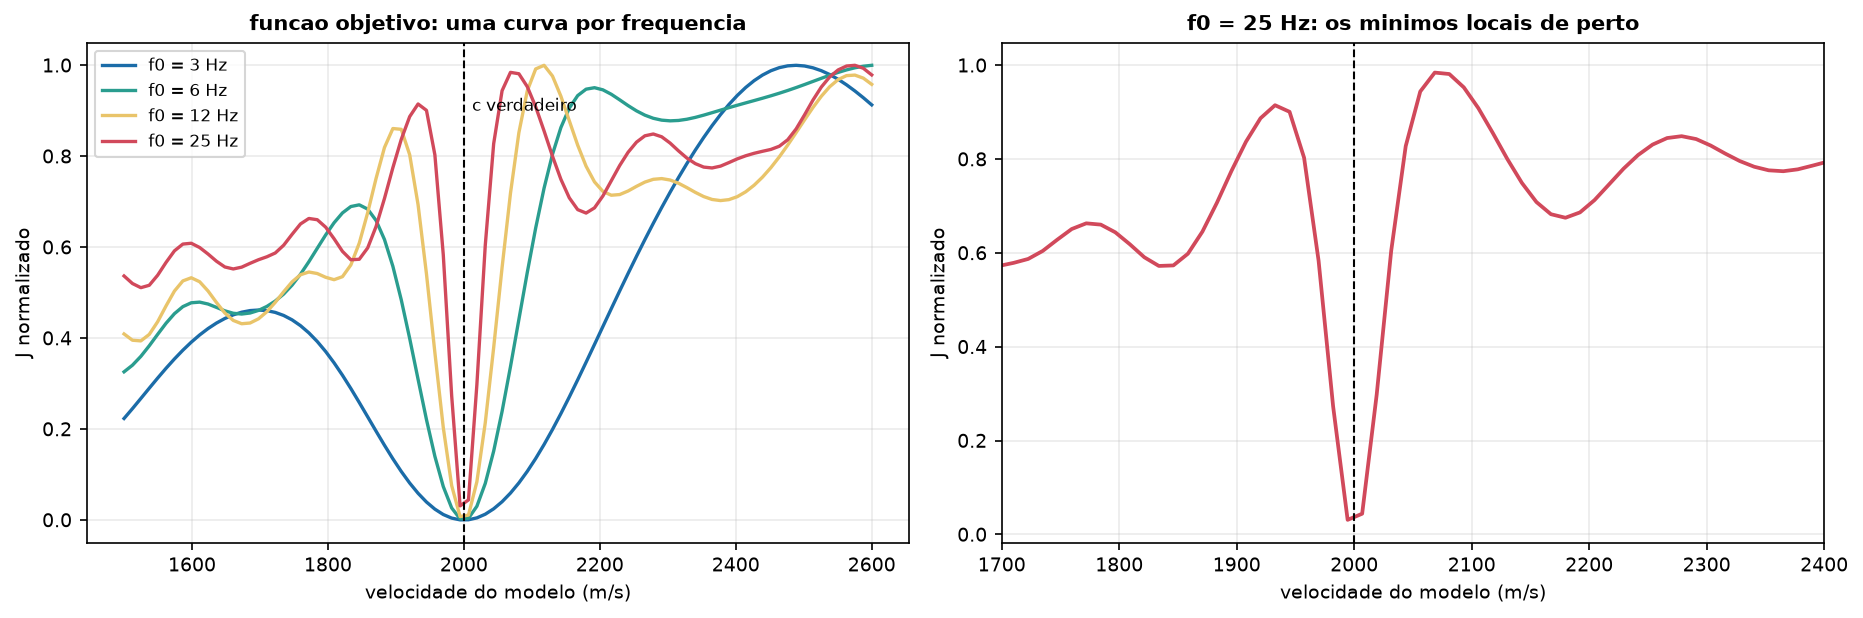
\includegraphics[width=0.96\textwidth]{../saidas/aula07/01_funcao_objetivo.png}
\caption{$J(c)$ varrido inteiro para quatro frequ\^encias, em meio
homog\^eneo com $c_{\text{verd}} = 2000$\,m/s --- poss\'ivel apenas porque
h\'a um \'unico par\^ametro. Em baixa frequ\^encia, um m\'inimo \'unico e
largo; em alta, um vale estreito cercado de m\'inimos locais.}
\end{figure}

\section{Cycle skipping: a explica\c{c}\~ao e o crit\'erio}

Se o modelo est\'a errado, o evento sint\'etico chega deslocado de $\delta t$
em rela\c{c}\~ao ao observado. Para um pulso aproximadamente harm\^onico de
per\'iodo $T$:

\begin{itemize}[leftmargin=*]
\item $\abs{\delta t} < T/2$: sint\'etico e observado ainda se sobrep\~oem no
\emph{mesmo} ciclo. O res\'iduo aponta na dire\c{c}\~ao certa.
\item $\abs{\delta t} > T/2$: o sint\'etico se alinha ao ciclo \emph{vizinho}.
O res\'iduo diminui ao empurrar o modelo para o lado \textbf{errado}.
\end{itemize}

\begin{equation}
\boxed{\;\abs{\delta t} < \frac{T}{2} = \frac{1}{2f}\;}
\label{eq:meiociclo}
\end{equation}

\begin{derivacao}[De \eqref{eq:meiociclo} \`a toler\^ancia em velocidade]
Para um percurso de comprimento $L$ atravessado com velocidade $c$, o tempo
\'e $t = L/c$. Com um erro $\delta c$ no modelo,
\[
\delta t = L\left(\frac{1}{c_{\text{ini}}} - \frac{1}{c_{\text{verd}}}\right)
 \approx -\frac{L\,\delta c}{c^{2}}
 \qquad (\delta c \ll c).
\]
Substituindo em \eqref{eq:meiociclo}:
\begin{equation}
\boxed{\;\abs{\delta c} < \frac{c^{2}}{2 f L}\;}
\label{eq:tolerancia}
\end{equation}
Note as tr\^es depend\^encias: a toler\^ancia cai com a \emph{frequ\^encia} e
com o \emph{comprimento do percurso}, e cresce com o \emph{quadrado} da
velocidade. Alvos profundos em meio lento s\~ao os mais dif\'iceis.
\end{derivacao}

\begin{center}
\begin{tabular}{@{}rrrr@{}}
\toprule
$f$ (Hz) & $T/2$ (ms) & $\abs{\delta c}_{\max}$ (m/s) & em \% \\
\midrule
2  & 250{,}0 & 667 & 33{,}3 \\
3  & 166{,}7 & 444 & 22{,}2 \\
5  & 100{,}0 & 267 & 13{,}3 \\
10 & 50{,}0  & 133 & 6{,}7 \\
20 & 25{,}0  & 67  & 3{,}3 \\
40 & 12{,}5  & 33  & 1{,}7 \\
\bottomrule
\end{tabular}
\end{center}
{\small ($L = 1500$\,m, $c = 2000$\,m/s)}

\subsection*{Valida\c{c}\~ao num\'erica do crit\'erio}

O curso mediu o \textbf{vale de atra\c{c}\~ao} de cada frequ\^encia --- o
conjunto de velocidades iniciais que converge para o m\'inimo certo --- e
comparou com \eqref{eq:tolerancia}, usando o percurso m\'edio
fonte--receptor da geometria do experimento ($L \approx 1580$\,m):

\begin{center}
\begin{tabular}{@{}rrrr@{}}
\toprule
$f_0$ (Hz) & vale medido (m/s) & semilargura prevista & semilargura medida \\
\midrule
3{,}0  & 1710 a 2489 & 422 & 389 \\
6{,}0  & 1858 a 2192 & 211 & 167 \\
12{,}0 & 1908 a 2118 & 105 & 105 \\
25{,}0 & 1945 a 2069 & 51  & 62 \\
\bottomrule
\end{tabular}
\end{center}

Uma conta de meia linha reproduz a largura medida e a depend\^encia $1/f$ ao
longo de uma faixa de $8\times$ em frequ\^encia. \'E raro uma regra
pr\'atica ser t\~ao bem comportada.

\begin{atencao}[Meio per\'iodo \'e uma aproxima\c{c}\~ao, e d\'a para medir
o qu\~ao boa]
O crit\'erio \eqref{eq:meiociclo} vale exatamente para um pulso harm\^onico.
Para uma ondaleta de banda finita, calcule $J$ em fun\c{c}\~ao do
deslocamento puro: para uma Ricker, a divisa entre ``corrige certo'' e
``corrige errado'' cai em $\delta t \approx 0{,}43\,T$, e existe um
\textbf{m\'inimo local esp\'urio} em $\delta t \approx 0{,}9\,T$ --- que \'e,
literalmente, o vale errado em que a invers\~ao fica presa.

Ou seja: \eqref{eq:meiociclo} \'e ligeiramente \textbf{otimista}. Use margem.
\end{atencao}

\begin{pratica}[Use isto antes de rodar]
Estime a frequ\^encia mais alta com que \emph{pode come\c{c}ar}, dada a
incerteza do modelo inicial. Se a tomografia tem 5\% de erro e o percurso
t\'ipico \'e 2\,km, com $c = 2000$\,m/s:
\[
\delta c = 100\ \text{m/s}
\;\Longrightarrow\;
f_{\max} = \frac{c^{2}}{2\,\delta c\,L}
 = \frac{2000^{2}}{2\cdot100\cdot2000} = 10\ \text{Hz}.
\]
Come\c{c}ar acima disso \'e desperd\'icio de tempo de m\'aquina.
\end{pratica}

\section{A estrat\'egia multiescala}

Da\'i decorre, sem mais nenhuma hip\'otese, a receita de Bunks \emph{et al.}
(1995): inverta primeiro nas frequ\^encias baixas, onde o vale \'e largo; use
o resultado como modelo inicial da banda seguinte; repita subindo.

\begin{lstlisting}
m = m_inicial
para cada banda f em [f_baixa ... f_alta]:
    d_filt = passa_baixa(d_obs, corte=f)     # Butterworth, tipicamente
    para it em 1..n_iter[f]:
        g   = gradiente(m, d_filt)           # Capitulo 6
        d_k = direcao(g, historico)          # Capitulo 8
        a   = busca_linear(m, d_k)           # Capitulo 8
        m   = m + a * d_k
    # reinicie o historico do l-BFGS ao trocar de banda
\end{lstlisting}

\begin{atencao}[Filtre os dois lados]
O filtro passa-baixa tem de ser aplicado ao dado observado \textbf{e} ao
sint\'etico, com \emph{exatamente} o mesmo filtro, dentro da avalia\c{c}\~ao
de $J$. Filtrar s\'o um dos dois introduz uma diferen\c{c}a de fase
sistem\'atica que a invers\~ao vai interpretar como estrutura.
\end{atencao}

\begin{teoria}[O limite honesto da multiescala]
A estrat\'egia s\'o resgata o que a banda \textbf{mais baixa} j\'a alcan\c{c}a.
Se o modelo inicial estiver fora do vale de atra\c{c}\~ao da menor
frequ\^encia \emph{dispon\'ivel no dado}, nenhuma ordem de bandas salva --- e
o Cap\'itulo~\ref{cap:completa} mostra um caso medido em que isso acontece.

O rem\'edio seria come\c{c}ar mais baixo ainda, o que exige dado com energia
nessas frequ\^encias. Da\'i o esfor\c{c}o da ind\'ustria em fontes de baixa
frequ\^encia: elas compram vale de atra\c{c}\~ao.
\end{teoria}

\section{O modelo inicial}

O modelo inicial precisa de uma \'unica coisa: estar dentro do vale de
atra\c{c}\~ao da menor frequ\^encia utiliz\'avel. Isso significa acertar os
\textbf{grandes} comprimentos de onda, n\~ao os detalhes.

\begin{armadilha}[Sobre testes sint\'eticos]
Usar o modelo verdadeiro suavizado como inicial \'e um teste
\textbf{generoso}: ele j\'a come\c{c}a dentro do vale por constru\c{c}\~ao.

N\~ao est\'a errado us\'a-lo para validar c\'odigo. Mas n\~ao confunda isso
com avaliar a \emph{robustez} do m\'etodo. Para isso, degrade o modelo inicial
de prop\'osito e descubra onde ele quebra.
\end{armadilha}

\section{Al\'em do $L_2$}

Como o problema \'e de fase, boa parte da pesquisa consiste em trocar o
funcional. As formas mais usadas, com a ideia de cada uma:

\begin{center}
\begin{tabular}{@{}lp{6.0cm}l@{}}
\toprule
\textbf{Funcional} & \textbf{Ideia} & \textbf{Pre\c{c}o} \\
\midrule
$L_2$ cl\'assico & $\tfrac12\int (d_{\text{cal}}-d_{\text{obs}})^{2}$
  & \emph{cycle skipping} \\
Envolt\'oria & \raggedright compara s\'o a envolt\'oria
  $E = \sqrt{d^{2} + (\mathcal{H}d)^{2}}$ ($\mathcal{H}$: transformada de
  Hilbert), insens\'ivel \`a fase fina & perde resolu\c{c}\~ao \\
Correla\c{c}\~ao cruzada & mede o \emph{deslocamento} $\Delta T$ que maximiza
  a correla\c{c}\~ao e penaliza $\Delta T^{2}$ & precisa janelar \\
Transporte \'otimo & dist\^ancia de Wasserstein entre sinais tratados como
  distribui\c{c}\~oes de massa: convexa em rela\c{c}\~ao a deslocamentos &
  exige positividade \\
Adaptativa (AWI) & estima o filtro de Wiener $u$ que leva o sint\'etico ao
  observado e penaliza $\norm{t\,u}^{2}/\norm{u}^{2}$ & mais par\^ametros \\
\bottomrule
\end{tabular}
\end{center}

\ponte{N\'ivel 3, Cap.\ 5}{cada funcional com a sua \textbf{fonte adjunta}
derivada --- que \'e a \'unica coisa que muda no c\'odigo --- e a discuss\~ao
de convexidade em rela\c{c}\~ao a deslocamento.}

\begin{pratica}[Ordem de prioridade quando a FWI n\~ao converge]
1.~Baixe a frequ\^encia inicial. \quad 2.~Melhore o modelo inicial. \quad
3.~\emph{S\'o ent\~ao} troque o funcional.

Trocar o funcional \'e a solu\c{c}\~ao mais cara e a que mais introduz
par\^ametros novos. Ela resolve casos em que 1 e 2 j\'a foram esgotados.
\end{pratica}

\begin{exercicio}
\begin{enumerate}[leftmargin=*, itemsep=2pt]
\item Deduza \eqref{eq:tolerancia} a partir de \eqref{eq:meiociclo} e
justifique a aproxima\c{c}\~ao usada.
\item O seu modelo inicial tem $8\%$ de erro, $c \approx 2500$\,m/s, percursos
de 3\,km. Qual a maior frequ\^encia inicial defens\'avel?
\item Por que filtrar apenas o dado observado (e n\~ao o sint\'etico)
corrompe a invers\~ao?
\end{enumerate}
\textbf{Respostas.} (1) $\delta t = L(1/c_{\text{ini}} - 1/c_{\text{verd}})$;
expandindo em torno de $c$ e mantendo o primeiro termo,
$\delta t \approx -L\delta c/c^{2}$, v\'alido para $\delta c \ll c$ ---
exatamente o regime em que se est\'a perto de convergir. (2) $\delta c = 200$\,m/s;
$f = c^{2}/(2\delta c L) = 6{,}25\times10^{6}/(1{,}2\times10^{6}) \approx
5{,}2$\,Hz. (3) Porque o filtro tem resposta de fase pr\'opria; aplicado a um
s\'o lado, ele cria um atraso sistem\'atico entre sint\'etico e observado que
a invers\~ao interpreta como erro de velocidade.
\end{exercicio}

% =====================================================================
\chapter{O m\'etodo do estado adjunto}
\label{cap:adjunto}

\begin{ideia}
Uma \'unica ideia --- escolher o multiplicador de Lagrange de modo a anular o
termo caro --- reduz o custo do gradiente de $N$ simula\c{c}\~oes para
\textbf{duas}, independentemente de $N$. Este cap\'itulo faz a dedu\c{c}\~ao
completa e a traduz linha a linha para c\'odigo.
\end{ideia}

\section{Por que n\~ao diferen\c{c}as finitas}
\label{sec:forcabruta}

O custo da abordagem ing\^enua \'e $N$ modelagens \emph{por itera\c{c}\~ao}:

\begin{center}
\begin{tabular}{@{}lrrr@{}}
\toprule
\textbf{Modelo} & $N$ & \textbf{modelagens/iter} & \textbf{tempo (a 0{,}4\,s cada)} \\
\midrule
$100\times100$   & 10\,000      & 10\,000      & 1{,}1 hora \\
$200\times400$   & 80\,000      & 80\,000      & 8{,}9 horas \\
$500\times1000$  & 500\,000     & 500\,000     & 2{,}3 dias \\
3D $300^{3}$     & 27\,000\,000 & 27\,000\,000 & 125 dias \\
\bottomrule
\end{tabular}
\end{center}

\begin{matematica}[multiplicadores de Lagrange, derivada funcional e operador adjunto]
A dedu\c{c}\~ao a seguir usa tr\^es ferramentas. Nenhuma \'e dif\'icil, mas a
combina\c{c}\~ao delas \'e o que torna a FWI poss\'ivel --- vale gastar uma
p\'agina antes.

\medskip
\textbf{1. Multiplicadores de Lagrange, em dimens\~ao finita.}
Para minimizar $f(\mathbf{x})$ sujeito a $\mathbf{c}(\mathbf{x}) = 0$,
constr\'oi-se
\[
\mathcal{L}(\mathbf{x},\boldsymbol{\lambda})
 = f(\mathbf{x}) + \boldsymbol{\lambda}^{T}\mathbf{c}(\mathbf{x}) .
\]
Como $\mathbf{c} = 0$ na solu\c{c}\~ao, $\mathcal{L} = f$ ali para
\emph{qualquer} $\boldsymbol{\lambda}$. Essa liberdade \'e o ponto: podemos
escolher $\boldsymbol{\lambda}$ do jeito que for mais conveniente.

\medskip
\textbf{2. O truque do adjunto, ainda em dimens\~ao finita.} \'E aqui que a
economia aparece. A vers\~ao cont\'inua, adiante, \'e esta mesma conta com
integrais no lugar de matrizes.

Queremos minimizar $f(\mathbf{u})$, com $\mathbf{u}$ n\~ao livre: ele resolve
um sistema que depende dos par\^ametros $\mathbf{q}$,
\[
A(\mathbf{q})\,\mathbf{u} = \mathbf{b}.
\]
Pela regra da cadeia,
$\dfrac{\dd f}{\dd q_j}
 = \dfrac{\partial f}{\partial \mathbf{u}}\,
   \dfrac{\dd\mathbf{u}}{\dd q_j}$,
e derivando a restri\c{c}\~ao,
$\dfrac{\dd\mathbf{u}}{\dd q_j}
 = -A^{-1}\dfrac{\partial A}{\partial q_j}\mathbf{u}$.

Calcular $\dd\mathbf{u}/\dd q_j$ exige \textbf{uma resolu\c{c}\~ao de sistema
por par\^ametro} --- \'e exatamente a for\c{c}a bruta da
§\ref{sec:forcabruta}. Mas observe a estrutura: o que queremos \'e o
\emph{produto} $\frac{\partial f}{\partial\mathbf{u}}A^{-1}(\cdots)$, e um
produto de tr\^es fatores pode ser associado de outro jeito. Definindo
$\boldsymbol{\lambda}$ por
\[
A^{T}\boldsymbol{\lambda}
 = -\left(\frac{\partial f}{\partial\mathbf{u}}\right)^{T}
\qquad\text{(\emph{uma} resolu\c{c}\~ao, com a matriz transposta)},
\]
o gradiente inteiro sai de uma vez:
\[
\frac{\dd f}{\dd q_j}
 = \boldsymbol{\lambda}^{T}\frac{\partial A}{\partial q_j}\mathbf{u} .
\]
\textbf{Duas resolu\c{c}\~oes} --- uma direta e uma transposta --- em vez de
$N$. O custo deixou de depender de $N$. Tudo o que vem a seguir \'e esta
conta, escrita para uma EDP.

\medskip
\textbf{3. Derivada funcional e integra\c{c}\~ao por partes.}
Quando a inc\'ognita \'e uma \emph{fun\c{c}\~ao}, a derivada vira
\textbf{derivada funcional}: perturbe $p \to p + \epsilon\,\delta p$ e recolha
o termo proporcional a $\epsilon$. Se o resultado tem a forma
$\int \Phi\,\delta p \dd t\dd\mathbf{x}$, ent\~ao
$\delta\mathcal{L}/\delta p = \Phi$; e exigir que a derivada se anule para
\emph{toda} perturba\c{c}\~ao equivale a exigir $\Phi = 0$ ponto a ponto.

Para chegar a essa forma \'e preciso tirar as derivadas de cima de $\delta p$.
A ferramenta \'e a integra\c{c}\~ao por partes,
\[
\int_0^T \lambda\,\partial_{tt}\delta p \dd t
 = \bigl[\lambda\,\partial_t\delta p - \partial_t\lambda\,\delta p\bigr]_0^T
 + \int_0^T \partial_{tt}\lambda\;\delta p \dd t ,
\]
e, no espa\c{c}o, a segunda identidade de Green,
\[
\int_\Omega \bigl(\lambda\nabla^{2}\delta p
 - \delta p\,\nabla^{2}\lambda\bigr)\dd\mathbf{x}
 = \oint_{\partial\Omega}\bigl(\lambda\,\partial_n\delta p
 - \delta p\,\partial_n\lambda\bigr)\dd S .
\]
Os colchetes e a integral de contorno s\~ao os \textbf{termos de fronteira}.
N\~ao s\~ao detalhe t\'ecnico: s\~ao o que define as condi\c{c}\~oes do
problema adjunto.

\medskip
\textbf{4. Operador adjunto.} $A^{*}$ \'e definido por
$\inner{Au}{v} = \inner{u}{A^{*}v}$ para todos $u,v$. Em dimens\~ao finita e
com o produto interno usual, $A^{*} = A^{T}$. A integra\c{c}\~ao por partes
acima \emph{\'e} o c\'alculo do adjunto: cada vez que uma derivada muda de
lado, est\'a se aplicando a defini\c{c}\~ao.

Um operador \'e \textbf{auto-adjunto} se $A^{*} = A$. O laplaciano com
condi\c{c}\~oes de contorno homog\^eneas \'e; $\partial_{tt}$ tamb\'em \'e; mas
$\partial_t$ \textbf{n\~ao} \'e --- ele troca de sinal,
$\partial_t^{*} = -\partial_t$. Essa \'ultima observa\c{c}\~ao explica,
sozinha, por que a equa\c{c}\~ao ac\'ustica sem atenua\c{c}\~ao \'e
revers\'ivel no tempo, e a viscoac\'ustica --- que tem uma derivada primeira
--- n\~ao \'e.
\end{matematica}

\section{A dedu\c{c}\~ao}
\label{sec:formulacao-grad}

Trabalhamos com $m(\mathbf{x}) = 1/c(\mathbf{x})^{2}$, porque a equa\c{c}\~ao
\'e linear nele. O problema direto entra como \textbf{restri\c{c}\~ao}:
\begin{equation}
\mathcal{F}(p,m) \;\equiv\; m\,\frac{\partial^{2}p}{\partial t^{2}}
 - \nabla^{2}p - s \;=\; 0 ,
\qquad p = \partial_t p = 0 \ \text{em } t=0 .
\end{equation}

\subsection*{Passo 1 --- o Lagrangiano}

A restri\c{c}\~ao vale para todo $\mathbf{x}$ e todo $t$, ent\~ao o
multiplicador \'e um \emph{campo} $\lambda(\mathbf{x},t)$:
\begin{equation}
\mathcal{L}(p, m, \lambda) = J(p) + \int_{\Omega}\!\!\int_{0}^{T}
\lambda\left[m\,\partial_{tt}p - \nabla^{2}p - s\right] \dd t\,\dd\mathbf{x}.
\label{eq:lagrangiano}
\end{equation}

Como a restri\c{c}\~ao \'e satisfeita pela solu\c{c}\~ao do problema direto,
$\mathcal{L} = J$ para qualquer $\lambda$ --- e podemos derivar $\mathcal{L}$
em vez de $J$, com a vantagem de podermos \emph{escolher} $\lambda$ para
eliminar o termo dif\'icil.

\begin{teoria}[Qual \'e o termo dif\'icil]
Pela regra da cadeia, $\dd J/\dd m = (\partial J/\partial p)(\partial p/
\partial m) + \partial J/\partial m$. O fator $\partial p/\partial m$ \'e uma
matriz $(\text{campo de onda}) \times (\text{par\^ametros})$: calcul\'a-la
coluna a coluna \'e exatamente a for\c{c}a bruta.

O truque do Lagrangiano \'e nunca calcular esse fator: escolhe-se $\lambda$
de modo que o coeficiente que o multiplica seja \emph{zero}.
\end{teoria}

\subsection*{Passo 2 --- varia\c{c}\~ao em rela\c{c}\~ao a $p$}

Escrevendo $J$ com deltas de Dirac nos receptores,
$J = \tfrac12\int\!\!\int \sum_r \delta(\mathbf{x}-\mathbf{x}_r)\,
(p - d_{\text{obs}})^{2}$, a sua varia\c{c}\~ao \'e
$\int\!\!\int \sum_r \delta(\mathbf{x}-\mathbf{x}_r)\,r\,\delta p$, com
$r = p - d_{\text{obs}}$ avaliado no receptor.

Na integral de \eqref{eq:lagrangiano}, integre por partes \textbf{duas vezes
no tempo} e \textbf{duas vezes no espa\c{c}o}:
\begin{align}
\int_{0}^{T}\!\lambda\,m\,\partial_{tt}\delta p \dd t
 &= \underbrace{\Bigl[\lambda m \partial_t \delta p
    - m\,\partial_t\lambda\,\delta p\Bigr]_{0}^{T}}_{(\star)}
  + \int_{0}^{T}\! m\,\partial_{tt}\lambda\;\delta p \dd t, \\
-\int_{\Omega}\lambda\,\nabla^{2}\delta p \dd\mathbf{x}
 &= \underbrace{-\oint_{\partial\Omega}
     \bigl(\lambda\,\partial_n \delta p
     - \delta p\,\partial_n\lambda\bigr)\dd S}_{(\star\star)}
  - \int_{\Omega} \nabla^{2}\lambda\;\delta p \dd\mathbf{x}.
\end{align}

\begin{atencao}[Os termos de fronteira, que quase todo texto omite]
$(\star)$ some em $t=0$ porque as condi\c{c}\~oes iniciais s\~ao fixas
($\delta p = \partial_t\delta p = 0$), e some em $t=T$ se impusermos
$\lambda = \partial_t\lambda = 0$ em $t = T$. \textbf{Essa \'e a origem das
condi\c{c}\~oes finais} do problema adjunto: elas n\~ao s\~ao uma
conven\c{c}\~ao, s\~ao o que faz a conta fechar.

$(\star\star)$ some se $\lambda$ obedecer, na fronteira de $\Omega$, ao
\emph{adjunto} da condi\c{c}\~ao de contorno do problema direto. Para
condi\c{c}\~oes de Dirichlet ($p=0$, superf\'icie livre) ou Neumann
homog\^eneas, a condi\c{c}\~ao adjunta \'e a mesma --- o operador \'e
auto-adjunto. Para uma CPML, \textbf{n\~ao \'e}, e ignorar isso \'e uma fonte
cl\'assica de erro silencioso no gradiente.
\end{atencao}

Restando apenas os termos proporcionais a $\delta p$:
\begin{equation}
\frac{\delta\mathcal{L}}{\delta p}
 = \bigl[m\,\partial_{tt}\lambda - \nabla^{2}\lambda\bigr]
 + \sum_{r} r(t)\,\delta(\mathbf{x}-\mathbf{x}_r).
\end{equation}

\subsection*{Passo 3 --- escolher $\lambda$: a equa\c{c}\~ao adjunta}

Exigindo $\delta\mathcal{L}/\delta p = 0$:
\begin{equation}
\boxed{\;
m\,\frac{\partial^{2}\lambda}{\partial t^{2}} - \nabla^{2}\lambda
 = -\sum_{r} r(t)\,\delta(\mathbf{x}-\mathbf{x}_r)\;}
\qquad
\lambda = \partial_t\lambda = 0 \ \text{em } t = T .
\label{eq:adjunta}
\end{equation}

\begin{teoria}[Leia a equa\c{c}\~ao adjunta]
\'E a \emph{mesma} equa\c{c}\~ao de onda do problema direto. Mudam duas
coisas:

\textbf{(1)} A fonte n\~ao \'e mais a ondaleta no ponto de tiro: \'e o
\textbf{res\'iduo}, com sinal trocado, injetado em \emph{todos} os receptores
simultaneamente. Cada receptor vira uma fonte.

\textbf{(2)} As condi\c{c}\~oes s\~ao \emph{finais}: resolve-se de tr\'as para
frente.

Interpreta\c{c}\~ao f\'isica: pega-se o erro que sobrou nos receptores e
joga-se de volta para dentro da Terra, para ver de onde ele veio.

Como a equa\c{c}\~ao ac\'ustica sem atenua\c{c}\~ao \'e \textbf{auto-adjunta}
(invariante por revers\~ao temporal), basta rodar o mesmo propagador ao
contr\'ario. Em meios dissipativos essa simetria se perde --- veja
§\ref{sec:adjunto-visco}.
\end{teoria}

\subsection*{Passo 4 --- varia\c{c}\~ao em rela\c{c}\~ao a $m$}

Com $\lambda$ escolhido, o \'unico termo que sobra em $\delta\mathcal{L}$ \'e
o expl\'icito em $m$:
\begin{equation}
\boxed{\;
\frac{\partial J}{\partial m}(\mathbf{x})
 = \int_{0}^{T} \lambda(\mathbf{x},t)\,
   \frac{\partial^{2}p}{\partial t^{2}}(\mathbf{x},t)\; \dd t \;}
\label{eq:gradiente}
\end{equation}
e, somando sobre os tiros, na forma discreta com os pesos de quadratura:
\begin{equation}
\frac{\partial J}{\partial m_i}
 = \Delta h^{2}\,\Delta t \sum_{s}\sum_{n}
   \lambda_i^{n}\,\bigl(\partial_{tt}p\bigr)_i^{n}.
\label{eq:gradiente_discreto}
\end{equation}

\begin{armadilha}[Os pesos de quadratura n\~ao s\~ao decorativos]
Esquecer $\Delta h^{2}\Delta t$ em \eqref{eq:gradiente_discreto} produz um
gradiente com a \emph{forma} certa e a \emph{escala} errada. A invers\~ao
ainda converge (a busca linear compensa com o passo), mas o teste do
Cap\'itulo~\ref{cap:verificacao} reprova, e qualquer compara\c{c}\~ao
quantitativa fica sem sentido.
\end{armadilha}

\begin{pratica}[O que essa f\'ormula \emph{\'e}]
Uma \textbf{correla\c{c}\~ao cruzada de defasagem zero} entre o campo direto
(sua segunda derivada temporal) e o campo adjunto, ponto a ponto.

O gradiente \'e grande onde os dois campos coincidem no tempo e no
espa\c{c}o --- isto \'e, nos pontos onde uma perturba\c{c}\~ao do modelo teria
afetado o dado.

Essa mesma estrutura \'e a condi\c{c}\~ao de imagem da migra\c{c}\~ao RTM. Em
ess\^encia, a RTM \'e a primeira itera\c{c}\~ao de uma FWI.
\end{pratica}

\section{Da f\'ormula ao c\'odigo}

\begin{lstlisting}
for s in tiros:
    # (1) DIRETO: resolve e guarda d2p/dt2
    d_calc, extras = solver.modelar(c, geom, wavelet, i_fonte=s,
                                    guardar_campo=True)
    # (2) RESIDUO
    Js, r = misfit_l2(d_calc, d_obs[:, :, s], dt);  J += Js
    # (3) ADJUNTO: mesma equacao, fonte = -residuo, de tras para frente
    lam = solver.retropropagar(c, geom, r)
    # (4) GRADIENTE: correlacao cruzada de defasagem zero
    g_ext += np.einsum("tzx,tzx->zx", lam, extras["dtt"]) * (dt * dh**2)

# (5) volta ao dominio fisico -- ADJUNTO da extensao de bordas
g_m = solver.contrair_adjunto(g_ext)
# (6) regra da cadeia para velocidade
g_c = g_m * (-2.0 / c**3)
\end{lstlisting}

\begin{armadilha}[O passo (5), que quase ningu\'em lembra]
O modelo f\'isico \'e estendido com a moldura absorvente antes de propagar, e
essa extens\~ao \emph{replica} os pixels de borda. Isso \'e um operador linear
$E$, e o gradiente precisa de $E^{T}$ --- a sensibilidade acumulada dentro da
moldura tem de ser \textbf{somada de volta} sobre o pixel de borda que a
gerou, n\~ao descartada com um recorte.

\begin{lstlisting}
# ERRADO -- descarta a sensibilidade acumulada na moldura
g_m = g_ext[topo:topo+nz, n:n+nx]

# CERTO -- E^T: dobra a moldura de volta sobre as bordas
g[topo]      += g[:topo].sum(axis=0)
g[topo+nz-1] += g[topo+nz:].sum(axis=0)
g[:, n]      += g[:, :n].sum(axis=1)
g[:, n+nx-1] += g[:, n+nx:].sum(axis=1)
\end{lstlisting}

Na montagem do curso, esse detalhe valia \textbf{9\% de erro} na derivada
direcional.
\end{armadilha}

\begin{teoria}[A regra geral]
\textbf{Toda opera\c{c}\~ao aplicada ao modelo antes de propagar precisa do
seu adjunto no caminho de volta do gradiente}: extens\~ao de bordas,
interpola\c{c}\~ao entre malhas, suaviza\c{c}\~ao, reparametriza\c{c}\~ao,
mudan\c{c}a de unidade.

Formalmente: se $\mvec_{\text{propaga}} = E\,\mvec$, ent\~ao
$\nabla_{\mvec} J = E^{T}\nabla_{\mvec_{\text{propaga}}} J$. Esquecer $E^{T}$
\'e o erro mais comum em c\'odigos de FWI caseiros.
\end{teoria}

\section{Armazenamento: \emph{checkpointing}}

O gradiente \eqref{eq:gradiente_discreto} exige o campo direto e o adjunto no
\emph{mesmo} instante --- mas o direto avan\c{c}a e o adjunto retrocede.

\begin{center}
\begin{tabular}{@{}llll@{}}
\toprule
\textbf{Estrat\'egia} & \textbf{Mem\'oria} & \textbf{Computa\c{c}\~ao}
& \textbf{Uso} \\
\midrule
Guardar tudo      & $n_t n_z n_x$     & 1 modelagem & 2D pequeno \\
Recomputar        & 1 campo           & $\sim n_t$  & nunca \\
\emph{Checkpointing} & $n_{chk} n_z n_x$ & $\sim 2$ & o padr\~ao \\
Revers\~ao de campo & contorno        & 2 & s\'o sem atenua\c{c}\~ao \\
\bottomrule
\end{tabular}
\end{center}

\begin{atencao}[Em 3D isso deixa de ser acad\^emico]
Um modelo $500\times500\times300$ com $n_t = 5000$ exigiria
\textbf{1{,}5\,TB por tiro} para guardar tudo. Por isso todo c\'odigo de FWI
3D usa \emph{checkpointing}.

E a revers\~ao de campo exige que o operador seja revers\'ivel no tempo. Sem
atenua\c{c}\~ao, \'e. \emph{Com} atenua\c{c}\~ao, n\~ao --- reconstruir o
campo direto rodando um meio dissipativo ao contr\'ario amplifica ru\'ido
exponencialmente (§\ref{sec:adjunto-visco}).
\end{atencao}

\section{Como ler um gradiente}

\begin{figure}[htbp]
\centering
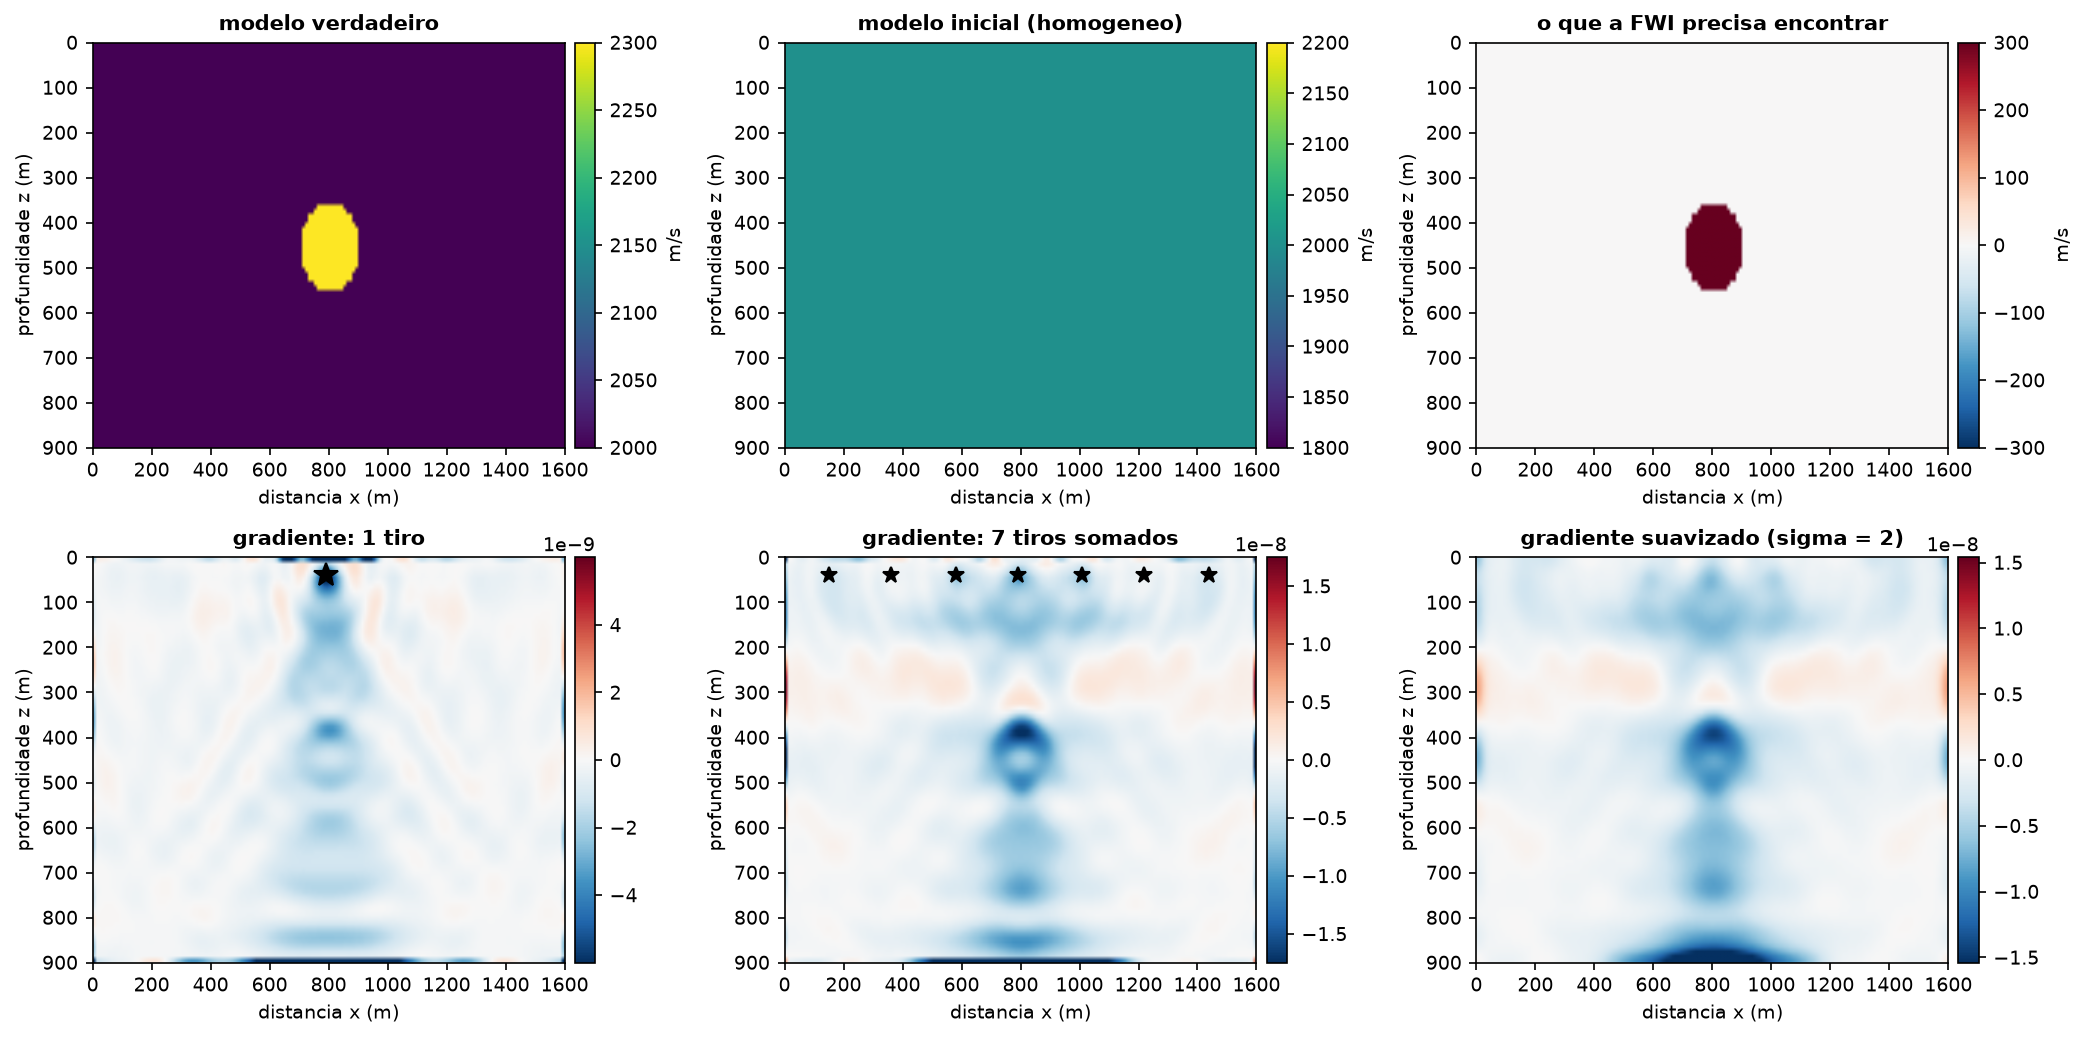
\includegraphics[width=0.96\textwidth]{../saidas/aula08/01_gradiente_adjunto.png}
\caption{Gradiente adjunto: um tiro (esquerda), sete tiros somados (centro) e
suavizado (direita). Um tiro isolado produz arcos amb\'iguos; \'e a soma sobre
tiros que localiza a anomalia.}
\end{figure}

\begin{enumerate}[leftmargin=*]
\item \textbf{O sinal --- e em qual par\^ametro.} A atualiza\c{c}\~ao \'e
$\mvec \leftarrow \mvec - \alpha\mathbf{g}$, e o sentido f\'isico depende do
par\^ametro. Em \textbf{velocidade}, $g_c < 0$ faz $c$ aumentar. Em
\textbf{vagarosidade ao quadrado} --- a forma em que \eqref{eq:gradiente} sai
--- o sentido se \textbf{inverte}, porque $\dd m/\dd c = -2/c^{3} < 0$: \'e
$g_m > 0$ que faz $c$ aumentar. Confira sempre contra uma perturba\c{c}\~ao
conhecida.
\item \textbf{Artefato perto de fontes e receptores.} O campo tem amplitude
enorme ali e a correla\c{c}\~ao explode. N\~ao \'e informa\c{c}\~ao: \'e
geometria. Mascare.
\item \textbf{Os arcos.} Um par fonte--receptor espalha a sensibilidade por
uma faixa. Ondas \emph{transmitidas} produzem a ``banana'' ligando fonte e
receptor; ondas \emph{espalhadas} produzem um arco de elipse --- a
is\'ocrona --- com focos na fonte e no receptor. A espessura, nos dois casos,
\'e a zona de Fresnel. Resolu\c{c}\~ao finita \'e consequ\^encia direta disso.
\item \textbf{Ilumina\c{c}\~ao decrescente com a profundidade.} Medida no
curso: raz\~ao raso/profundo de \textbf{181$\times$}. Sem corre\c{c}\~ao, a
FWI s\'o atualiza a parte rasa.
\end{enumerate}

\begin{exercicio}
\begin{enumerate}[leftmargin=*, itemsep=2pt]
\item Por que as condi\c{c}\~oes do problema adjunto s\~ao \emph{finais} e
n\~ao iniciais? Aponte o termo exato da dedu\c{c}\~ao.
\item Escreva $\partial J/\partial c$ diretamente, sem passar por $m$, e
explique por que a forma em $m$ \'e prefer\'ivel.
\item O seu c\'odigo suaviza o modelo com um filtro gaussiano $S$ antes de
propagar. O que precisa mudar no gradiente?
\end{enumerate}
\textbf{Respostas.} (1) O termo $(\star)$ avaliado em $t=T$: impor
$\lambda = \partial_t\lambda = 0$ ali \'e o que o anula, j\'a que $\delta p$
em $t=T$ \'e livre. (2) $\partial J/\partial c = (-2/c^{3})\int\lambda\,
\partial_{tt}p\dd t$; a forma em $m$ \'e prefer\'ivel porque a equa\c{c}\~ao
\'e linear em $m$, de modo que $\partial\mathcal{F}/\partial m = \partial_{tt}p$
sai sem regra da cadeia. (3) O gradiente precisa de $S^{T}$ --- que, para um
filtro gaussiano sim\'etrico, \'e o pr\'oprio $S$; mas isso \emph{precisa} ser
aplicado, n\~ao presumido.
\end{exercicio}

% =====================================================================
\chapter{Verifica\c{c}\~ao do gradiente}
\label{cap:verificacao}

\begin{ideia}
Um gradiente errado n\~ao gera erro nem trava o programa: gera uma invers\~ao
que roda at\'e o fim e devolve um modelo plaus\'ivel e errado. Existem tr\^es
testes, de custo baixo, que separam ``o c\'odigo roda'' de ``o c\'odigo
est\'a certo'' --- e o terceiro deles \'e conclusivo.
\end{ideia}

\section{O modo de falha silencioso}

\begin{armadilha}[Por que o erro n\~ao aparece]
Um gradiente errado geralmente ainda \'e uma dire\c{c}\~ao de descida
\emph{aproximada}. A busca linear encontra um passo que reduz $J$, a curva de
converg\^encia desce, e o modelo final tem estrutura.

Nenhum dos sintomas normais aparece. Voc\^e descobre quando algu\'em tenta
reproduzir --- ou quando o resultado n\~ao bate com um po\c{c}o. Por isso a
verifica\c{c}\~ao \'e \textbf{obrigat\'oria}, e antes da primeira invers\~ao.
\end{armadilha}

\section{Teste 1 --- diferen\c{c}as finitas pontuais}

Compara $\partial J/\partial m_i$ em alguns pixels com a mexida bruta:
\begin{equation}
\frac{\partial J}{\partial m_i} \;\stackrel{?}{\approx}\;
\frac{J(\mvec + \varepsilon\mathbf{e}_i) - J(\mvec - \varepsilon\mathbf{e}_i)}
     {2\varepsilon}.
\end{equation}

Serve para \textbf{localizar} onde o gradiente erra --- n\~ao para aprovar ou
reprovar. Resultado medido pelo curso:

\begin{center}
\begin{tabular}{@{}lrrrr@{}}
\toprule
\textbf{Ponto} & $\abs{g}$ relativo & \textbf{Adjunto} & \textbf{Dif.\ finitas}
& \textbf{Raz\~ao} \\
\midrule
(0, 50)  & $1{,}0$              & $4{,}7484\times10^{1}$  & $4{,}7489\times10^{1}$  & 0{,}9999 \\
(17, 89) & $5{,}1\times10^{-1}$ & $-2{,}4217\times10^{1}$ & $-2{,}4219\times10^{1}$ & 0{,}9999 \\
(34, 89) & $2{,}1\times10^{-1}$ & $9{,}8459$              & $9{,}8452$              & 1{,}0001 \\
(14, 21) & $8{,}7\times10^{-2}$ & $-4{,}1222$             & $-4{,}1195$             & 1{,}0006 \\
(38, 27) & $1{,}0\times10^{-7}$ & $4{,}86\times10^{-6}$   & $4{,}28\times10^{-3}$   & 0{,}0011 \\
\bottomrule
\end{tabular}
\end{center}

\begin{atencao}[A \'ultima linha \'e instrutiva, e n\~ao \'e um \emph{bug}]
Num ponto de gradiente desprez\'ivel, numerador e denominador s\~ao ambos da
ordem do ru\'ido de \texttt{float32}, e a raz\~ao entre eles n\~ao significa
nada. Isso \textbf{n\~ao} \'e erro de gradiente: \'e o limite de precis\~ao do
pr\'oprio teste.

Sempre pondere o teste pontual pela magnitude local de $\abs{g}$, e nunca
reprove um c\'odigo por causa de um ponto de sensibilidade nula.
\end{atencao}

\section{Teste 2 --- derivada direcional}

Compara $\inner{\mathbf{g}}{\mathbf{h}}$ com a diferen\c{c}a centrada ao longo
de uma dire\c{c}\~ao $\mathbf{h}$:
\begin{equation}
\rho(\alpha) = \frac{\inner{\mathbf{g}}{\mathbf{h}}}
  {\bigl[J(\mvec+\alpha\mathbf{h}) - J(\mvec-\alpha\mathbf{h})\bigr]/2\alpha}
\;\stackrel{?}{\to}\; 1 .
\end{equation}

Testa o gradiente \emph{inteiro} em um n\'umero s\'o, e custa 2 modelagens por
$\alpha$. \'E o teste do dia a dia.

\begin{center}
\begin{tabular}{@{}rrr@{}}
\toprule
$\alpha$ & \textbf{Num\'erico (centrado)} & \textbf{Raz\~ao} \\
\midrule
0{,}4  & $4{,}56559876\times10^{-6}$ & 1{,}000661 \\
0{,}2  & $4{,}56776551\times10^{-6}$ & 1{,}000186 \\
0{,}1  & $4{,}56870921\times10^{-6}$ & 0{,}999980 \\
0{,}05 & $4{,}56812642\times10^{-6}$ & 1{,}000107 \\
0{,}02 & $4{,}57093344\times10^{-6}$ & 0{,}999493 \\
0{,}01 & $4{,}56566693\times10^{-6}$ & 1{,}000646 \\
\bottomrule
\end{tabular}
\end{center}
{\small Erro m\'aximo: $0{,}07\%$.}

\begin{atencao}[A escolha da dire\c{c}\~ao $\mathbf{h}$]
Uma dire\c{c}\~ao \emph{aleat\'oria} \'e quase ortogonal ao gradiente (que \'e
suave), o que deixa $\inner{\mathbf{g}}{\mathbf{h}}$ pequeno e o teste
dominado por arredondamento e pelos termos de ordem superior (a curvatura em
si se cancela na diferen\c{c}a centrada). Use uma dire\c{c}\~ao \textbf{suave} --- o pr\'oprio
gradiente normalizado \'e a escolha mais confi\'avel.
\end{atencao}

\begin{matematica}[ordem de converg\^encia, e como l\^e-la num gr\'afico log-log]
Este teste n\~ao compara \emph{valores}: compara \emph{taxas}. A ferramenta
\'e a mesma da §\ref{sec:taylor-fd}, usada de outro jeito.

Se um erro se comporta como $E(\alpha) = C\alpha^{n}$, ent\~ao
$\log E = \log C + n\log\alpha$: em eixos logar\'itmicos, \'e uma
\textbf{reta de inclina\c{c}\~ao $n$}. Medir $n$ \'e medir a
inclina\c{c}\~ao --- ou, numericamente,
\[
n \approx \frac{\log\bigl(E(\alpha_1)/E(\alpha_2)\bigr)}
               {\log(\alpha_1/\alpha_2)} .
\]

A gra\c{c}a do m\'etodo \'e que a inclina\c{c}\~ao \textbf{n\~ao depende de
$C$}: voc\^e n\~ao precisa saber o valor certo da derivada, nem a escala do
problema, nem calibrar nada. Basta que a reta tenha a inclina\c{c}\~ao
prevista pela teoria. \'E o que torna este teste conclusivo, e n\~ao apenas
indicativo.
\end{matematica}

\section{Teste 3 --- teste de Taylor (o conclusivo)}

N\~ao compara valores: compara \textbf{taxas de converg\^encia}.
\begin{align}
E_0(\alpha) &= \bigl|J(\mvec+\alpha\mathbf{h}) - J(\mvec)\bigr|
 \;\sim\; \mathcal{O}(\alpha), \\
E_1(\alpha) &= \bigl|J(\mvec+\alpha\mathbf{h}) - J(\mvec)
 - \alpha\inner{\mathbf{g}}{\mathbf{h}}\bigr|
 \;\sim\; \mathcal{O}(\alpha^{2}).
\end{align}

\begin{derivacao}[Por que $\mathcal{O}(\alpha^{2})$ prova que o gradiente
\'e exato]
Por Taylor,
$J(\mvec+\alpha\mathbf{h}) = J(\mvec)
 + \alpha\inner{\nabla J}{\mathbf{h}}
 + \tfrac{\alpha^{2}}{2}\mathbf{h}^{T}H\mathbf{h} + \mathcal{O}(\alpha^{3})$.
Ent\~ao
\[
E_1(\alpha) = \Bigl|\alpha\inner{\nabla J - \mathbf{g}}{\mathbf{h}}
 + \tfrac{\alpha^{2}}{2}\mathbf{h}^{T}H\mathbf{h} + \dots\Bigr| .
\]
Se $\mathbf{g} = \nabla J$, o termo linear desaparece e sobra
$\mathcal{O}(\alpha^{2})$. Se $\mathbf{g} \ne \nabla J$, o termo linear
sobrevive e $E_1 \sim \mathcal{O}(\alpha)$.

\textbf{Este \'e o diagn\'ostico mais informativo que existe}, e n\~ao exige
conhecer a resposta certa: basta observar a inclina\c{c}\~ao em escala log-log.
\end{derivacao}

\begin{center}
\begin{tabular}{@{}rrrrr@{}}
\toprule
$\alpha$ & $E_0$ & $E_1$ & ordem $E_0$ & ordem $E_1$ \\
\midrule
0{,}4   & $2{,}285\times10^{-6}$ & $4{,}578\times10^{-7}$ & --- & --- \\
0{,}2   & $1{,}028\times10^{-6}$ & $1{,}146\times10^{-7}$ & 1{,}15 & \textbf{2{,}00} \\
0{,}1   & $4{,}855\times10^{-7}$ & $2{,}867\times10^{-8}$ & 1{,}08 & \textbf{2{,}00} \\
0{,}05  & $2{,}355\times10^{-7}$ & $7{,}116\times10^{-9}$ & 1{,}04 & \textbf{2{,}01} \\
0{,}025 & $1{,}160\times10^{-7}$ & $1{,}756\times10^{-9}$ & 1{,}02 & \textbf{2{,}02} \\
\bottomrule
\end{tabular}
\end{center}

\begin{figure}[htbp]
\centering
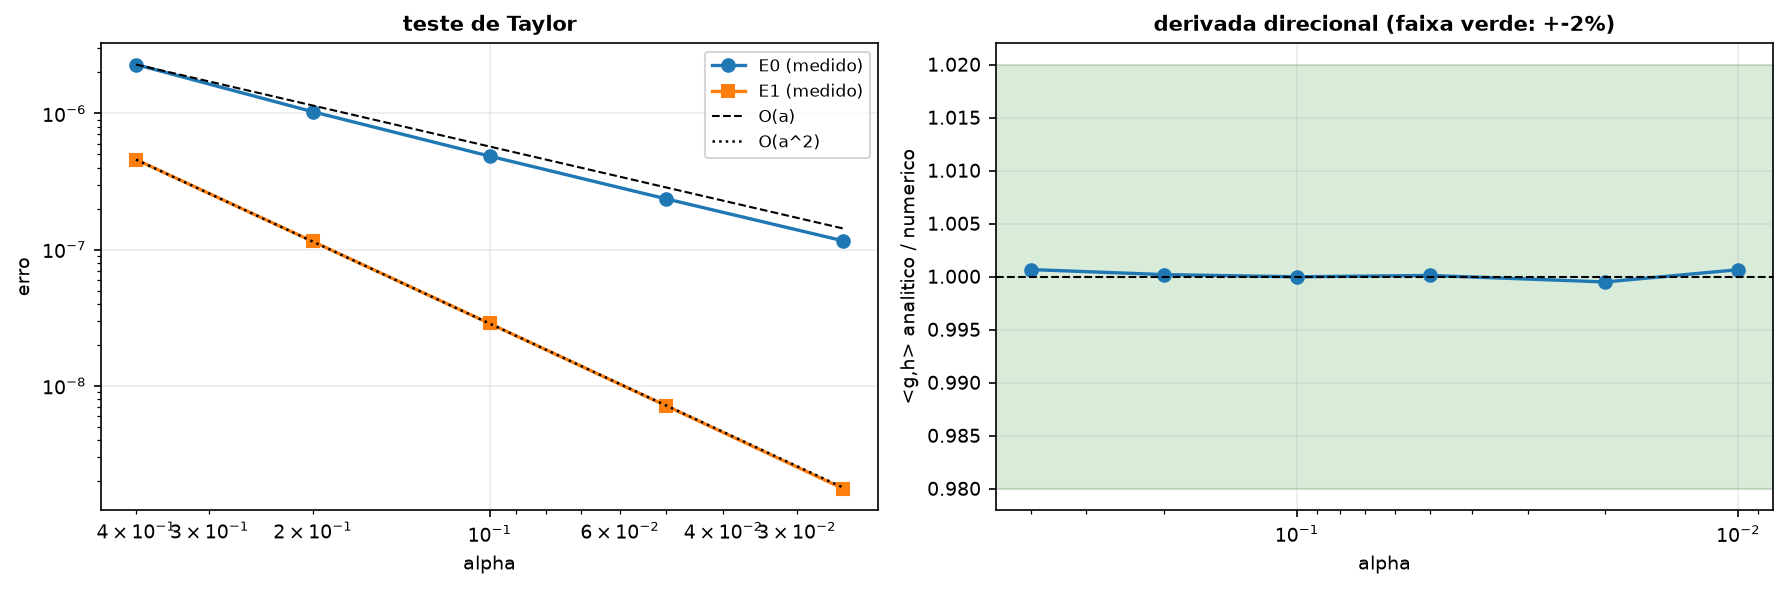
\includegraphics[width=0.96\textwidth]{../saidas/aula09/01_testes_de_gradiente.png}
\caption{Esquerda: teste de Taylor em log-log, com as retas de refer\^encia
$\mathcal{O}(\alpha)$ e $\mathcal{O}(\alpha^{2})$. Direita: raz\~ao da
derivada direcional; faixa verde de $\pm 2\%$.}
\end{figure}

\section{Diagnosticar pelo padr\~ao}

\begin{center}
\begin{tabular}{@{}lp{9.2cm}@{}}
\toprule
\textbf{Padr\~ao} & \textbf{Diagn\'ostico} \\
\midrule
$\rho \approx 1$, est\'avel & gradiente correto \\
$\rho$ est\'avel mas $\ne 1$ & erro \textbf{sistem\'atico}: fator de escala
esquecido, sinal trocado, peso de quadratura ($\Delta t$, $\Delta h^{2}$)
faltando, termo ausente no adjunto, ou adjunto de um pr\'e-processamento
omitido. Valor est\'avel \'e boa not\'icia: o \emph{bug} \'e determin\'istico \\
$\rho$ inst\'avel & ru\'ido num\'erico: $\alpha$ pequeno demais para a
precis\~ao usada. Aumente $\alpha$ ou use precis\~ao dupla \\
$E_1 \sim \mathcal{O}(\alpha)$ & o gradiente \emph{n\~ao} \'e a derivada:
sobrou termo de primeira ordem \\
\bottomrule
\end{tabular}
\end{center}

\section{Estudo de caso: o \emph{bug} que estes testes encontraram}

Vale o relato completo, porque mostra os tr\^es testes se complementando.

O propagador do curso \textbf{reprovou} no teste da derivada direcional, com
raz\~ao $0{,}9118$ em \emph{todos} os $\alpha$, ao longo de uma faixa de
$40\times$:

\begin{center}
\begin{tabular}{@{}rrr@{}}
\toprule
$\alpha$ & num\'erico & raz\~ao \\
\midrule
0{,}4  & $2{,}41766\times10^{-6}$ & 0{,}911797 \\
0{,}2  & $2{,}41808\times10^{-6}$ & 0{,}911639 \\
0{,}1  & $2{,}41747\times10^{-6}$ & 0{,}911871 \\
0{,}05 & $2{,}41784\times10^{-6}$ & 0{,}911728 \\
0{,}02 & $2{,}41946\times10^{-6}$ & 0{,}911119 \\
0{,}01 & $2{,}41739\times10^{-6}$ & 0{,}911900 \\
\bottomrule
\end{tabular}
\end{center}

Estabilidade perfeita descarta ru\'ido num\'erico e aponta erro
sistem\'atico. O teste \textbf{pontual} localizou a regi\~ao: raz\~ao
$\approx 0{,}99$ no miolo do modelo e $\approx 0{,}72$ perto da superf\'icie.
O erro estava nas bordas --- era exatamente o $E^{T}$ omitido, descrito no
Cap\'itulo~\ref{cap:adjunto}. Com a corre\c{c}\~ao, a raz\~ao passou de
$0{,}9118$ para $1{,}0001$.

\begin{pratica}[Protocolo m\'inimo, a rodar sempre que o c\'odigo mudar]
\begin{enumerate}[leftmargin=*, itemsep=1pt]
\item Modelo pequeno (50$\times$100 basta), poucos tiros, $f_0$ moderado.
\item Direcional com 5--6 valores de $\alpha$ cobrindo duas ordens de
grandeza. Se $\rho \ne 1$, \textbf{pare e conserte}.
\item Taylor: confirme inclina\c{c}\~ao 2 em log-log.
\item Pontual apenas se 2 ou 3 falharem, para localizar.
\end{enumerate}
Custa minutos. Um gradiente errado custa semanas.
\end{pratica}

% =====================================================================
\chapter{Otimiza\c{c}\~ao}
\label{cap:otimizacao}

\begin{ideia}
Todos os m\'etodos t\^em a forma $\mvec_{k+1} = \mvec_k + \alpha_k\mathbf{d}_k$.
O que muda \'e quanta informa\c{c}\~ao de \textbf{curvatura} se usa para
construir $\mathbf{d}_k$ --- e, como a Hessiana \'e impens\'avel neste
tamanho, toda a arte est\'a em aproxim\'a-la de gra\c{c}a.
\end{ideia}

\begin{matematica}[o modelo quadr\'atico local: gradiente, Hessiana e dire\c{c}\~ao de descida]
Todo m\'etodo de otimiza\c{c}\~ao responde \`a mesma pergunta: se eu s\'o
enxergo a vizinhan\c{c}a do ponto onde estou, qual \'e o melhor palpite sobre
onde fica o fundo?

\textbf{O modelo local.} Expandindo $J$ em torno de $\mvec$:
\[
J(\mvec + \delta) \approx J(\mvec)
 + \inner{\mathbf{g}}{\delta}
 + \tfrac{1}{2}\,\delta^{T}H\,\delta ,
\qquad
\mathbf{g} = \nabla J,\quad
H_{ij} = \frac{\partial^{2}J}{\partial m_i\,\partial m_j}.
\]
O \textbf{gradiente} \'e a inclina\c{c}\~ao; a \textbf{Hessiana} \'e a
curvatura. Minimizar o lado direito d\'a o passo de Newton
$\delta = -H^{-1}\mathbf{g}$, e todos os m\'etodos deste cap\'itulo s\~ao
aproxima\c{c}\~oes dele.

\textbf{Dire\c{c}\~ao de descida.} $\mathbf{d}$ \'e dire\c{c}\~ao de descida
se $\inner{\mathbf{g}}{\mathbf{d}} < 0$ --- andar um pouquinho nela reduz $J$.
O gradiente negativo sempre serve; qualquer $-P\mathbf{g}$ com $P$
\textbf{positiva definida} tamb\'em serve, porque
$\inner{\mathbf{g}}{-P\mathbf{g}} = -\mathbf{g}^{T}P\mathbf{g} < 0$. \'E por
isso que toda aproxima\c{c}\~ao da inversa da Hessiana precisa ser mantida
positiva definida: \'e o que garante que o m\'etodo continue descendo.

\textbf{Positiva definida} significa $\mathbf{v}^{T}P\mathbf{v} > 0$ para todo
$\mathbf{v}\ne 0$ --- geometricamente, que a superf\'icie local \'e uma tigela
em todas as dire\c{c}\~oes, sem sela nem vale plano.

\textbf{Condicionamento.} A raz\~ao entre o maior e o menor autovalor de $H$
\'e o \emph{n\'umero de condi\c{c}\~ao}, e mede o qu\~ao alongado \'e o vale:
condi\c{c}\~ao 1 \'e uma tigela circular (a descida m\'axima acerta de
primeira); condi\c{c}\~ao $10^{4}$ \'e um desfiladeiro (ela ziguezagueia).
\textbf{Pr\'e-condicionar \'e tentar deixar o vale mais redondo} --- nada
al\'em disso.
\end{matematica}

\section{O panorama}

\begin{center}
\begin{tabular}{@{}llll@{}}
\toprule
\textbf{M\'etodo} & $\mathbf{d}_k$ & \textbf{Mem\'oria} & \textbf{Em FWI} \\
\midrule
Newton           & $-H^{-1}\mathbf{g}$ & $N^{2}$ & imposs\'ivel \\
Gauss--Newton    & $-(J'^{T}J')^{-1}\mathbf{g}$ & $N^{2}$ & s\'o truncado \\
Descida m\'axima & $-\mathbf{g}$ & $N$ & barato, lento \\
Grad.\ conjugado & $-\mathbf{g} + \beta_k\mathbf{d}_{k-1}$ & $2N$ & bom
  custo/benef\'icio \\
l-BFGS           & $-H_{\text{aprox}}\mathbf{g}$ & $2\ell N$ & \textbf{o padr\~ao} \\
\bottomrule
\end{tabular}
\end{center}

Com $N = 10^{6}$, a Hessiana tem $10^{12}$ entradas: 4\,TB em
\texttt{float32}. N\~ao se monta, n\~ao se armazena, n\~ao se inverte.

Mas a Hessiana \textbf{importa}: na diagonal, a ilumina\c{c}\~ao de cada
ponto; fora dela, o acoplamento entre pontos do modelo (e, em
multipar\^ametro, entre par\^ametros). Os m\'etodos quase-Newton existem para
capturar parte disso sem montar a matriz.

\subsection*{Gradiente conjugado n\~ao linear}

\begin{equation}
\mathbf{d}_k = -\mathbf{g}_k + \beta_k \mathbf{d}_{k-1},
\qquad
\beta_k^{\text{FR}} = \frac{\norm{\mathbf{g}_k}^{2}}{\norm{\mathbf{g}_{k-1}}^{2}},
\qquad
\beta_k^{\text{PR}} = \frac{\inner{\mathbf{g}_k}{\mathbf{g}_k-\mathbf{g}_{k-1}}}
  {\norm{\mathbf{g}_{k-1}}^{2}} .
\end{equation}

Na pr\'atica usa-se Polak--Ribière com salvaguarda
$\beta_k = \max(\beta_k^{\text{PR}}, 0)$, o que equivale a
\emph{reiniciar} o m\'etodo (voltar \`a descida m\'axima) sempre que a
f\'ormula produziria uma dire\c{c}\~ao ruim.

\subsection*{l-BFGS: a recurs\~ao de dois la\c{c}os}

O l-BFGS constr\'oi uma aproxima\c{c}\~ao da \emph{inversa} da Hessiana usando
apenas os \'ultimos $\ell$ pares
$\mathbf{s}_k = \mvec_{k+1}-\mvec_k$ e
$\mathbf{y}_k = \mathbf{g}_{k+1}-\mathbf{g}_k$, sem nunca formar matriz
alguma:

\begin{lstlisting}
# entrada: g (gradiente atual), pares (s_i, y_i), i = k-1 ... k-l
q = g
for i in [k-1, ..., k-l]:                 # primeiro laco (para tras)
    rho_i  = 1.0 / dot(y_i, s_i)
    alpha_i = rho_i * dot(s_i, q)
    q      = q - alpha_i * y_i

gamma = dot(s_{k-1}, y_{k-1}) / dot(y_{k-1}, y_{k-1})
r = gamma * q                             # H0 = gamma * I  (escalamento)

for i in [k-l, ..., k-1]:                 # segundo laco (para frente)
    beta_i = rho_i * dot(y_i, r)
    r      = r + s_i * (alpha_i - beta_i)

d = -r                                    # direcao de busca
\end{lstlisting}

O custo \'e $4\ell N$ opera\c{c}\~oes e $2\ell N$ de mem\'oria; com
$\ell = 5$ a $20$, isso \'e desprez\'ivel diante de uma modelagem.

\begin{atencao}[Dois cuidados que resolvem a maioria dos problemas]
\textbf{1. Reinicie o hist\'orico ao trocar de banda de frequ\^encia} na
multiescala. Os pares $(\mathbf{s},\mathbf{y})$ descrevem a curvatura do
problema \emph{antigo}; mantidos, atrapalham.

\textbf{2. Rejeite pares com $\inner{\mathbf{y}}{\mathbf{s}} \le 0$.} A
condi\c{c}\~ao de curvatura $\inner{\mathbf{y}}{\mathbf{s}} > 0$ \'e o que
garante que a aproxima\c{c}\~ao seja positiva definida --- e, portanto, que
$\mathbf{d}_k$ seja dire\c{c}\~ao de descida. Ela \'e satisfeita
automaticamente se a busca linear cumprir as condi\c{c}\~oes de Wolfe.
\end{atencao}

\section{A busca linear, onde o tempo \'e gasto}

Achar a dire\c{c}\~ao \'e metade do trabalho; decidir \emph{quanto andar} \'e
a outra. Em FWI cada tentativa custa uma modelagem completa de todos os tiros.

\begin{align}
&\text{(Armijo, decr\'escimo suficiente)}
&& J(\mvec + \alpha\mathbf{d}) \le J(\mvec)
 + c_1\alpha\inner{\mathbf{g}}{\mathbf{d}}, \\
&\text{(curvatura, 2\textsuperscript{a} cond.\ de Wolfe)}
&& \inner{\nabla J(\mvec+\alpha\mathbf{d})}{\mathbf{d}}
 \ge c_2\inner{\mathbf{g}}{\mathbf{d}},
\end{align}
tipicamente $c_1 = 10^{-4}$ e $c_2 = 0{,}9$.

\begin{pratica}[Duas estrat\'egias, e quando usar cada uma]
\textbf{Retrocesso (\emph{backtracking}).} Tente $\alpha$; se Armijo falhar,
$\alpha \leftarrow \alpha/2$. Simples e robusto, gasta 5--10 avalia\c{c}\~oes.
Use quando o gradiente ainda n\~ao \'e confi\'avel.

\textbf{Ajuste parab\'olico.} J\'a se conhece $J(0)$ e a inclina\c{c}\~ao
$\inner{\mathbf{g}}{\mathbf{d}}$; com \emph{uma} avalia\c{c}\~ao extra fica
determinada a par\'abola
\[
q(\alpha) = J_0 + \inner{\mathbf{g}}{\mathbf{d}}\,\alpha + c\,\alpha^{2},
\qquad
\alpha^{*} = -\frac{\inner{\mathbf{g}}{\mathbf{d}}}{2c},
\]
cujo m\'inimo d\'a o passo. Acerta em $\sim$2 avalia\c{c}\~oes. \'E o padr\~ao
depois que o c\'odigo est\'a verificado.
\end{pratica}

\begin{atencao}[O chute inicial do passo]
O crit\'erio com significado f\'isico: \emph{n\~ao altere o modelo em mais de
1--3\% de uma vez}. Isso \'e mais confi\'avel que qualquer estimativa
puramente matem\'atica, porque respeita a escala do problema. Em pr\'atica:
\[
\alpha_0 = \frac{0{,}02\,\max\abs{\mvec}}{\max\abs{\mathbf{d}}} .
\]
\end{atencao}

\section{A Hessiana e o pr\'e-condicionamento}

\begin{derivacao}[A estrutura da Hessiana de m\'inimos quadrados]
Com $J = \tfrac12\norm{\mathbf{r}(\mvec)}^{2}$ e $J' = \partial\mathbf{r}/
\partial\mvec$ (a matriz de sensibilidade, ou jacobiana),
\begin{equation}
\mathbf{g} = J'^{T}\mathbf{r},
\qquad
H = \underbrace{J'^{T}J'}_{H_{\text{GN}}}
  + \underbrace{\sum_i r_i \nabla^{2} r_i}_{\text{termo de segunda ordem}} .
\label{eq:hessiana}
\end{equation}

A aproxima\c{c}\~ao de \textbf{Gauss--Newton} descarta o segundo termo, o que
\'e justific\'avel quando os res\'iduos s\~ao pequenos ou o problema \'e
quase linear. $H_{\text{GN}}$ \'e sempre semidefinida positiva --- da\'i a sua
popularidade.

Em FWI, o termo descartado cont\'em a informa\c{c}\~ao sobre \emph{m\'ultiplo
espalhamento}: ele \'e o que distingue uma reflex\~ao de segunda ordem de uma
estrutura nova. Ignor\'a-lo \'e barato e quase sempre aceit\'avel; saber que
foi ignorado \'e obrigat\'orio.
\end{derivacao}

\begin{teoria}[O que o pr\'e-condicionamento realmente \'e]
A atualiza\c{c}\~ao ideal de Newton seria
$\delta\mvec = -H^{-1}\mathbf{g}$. O pr\'e-condicionador $P$ \'e uma
aproxima\c{c}\~ao \emph{barata} de $H^{-1}$.

A diagonal de $H_{\text{GN}}$ \'e bem aproximada pela \textbf{energia do campo
direto} em cada ponto --- a ilumina\c{c}\~ao. A aproxima\c{c}\~ao tem nome e
refer\^encia: \'e o \emph{pseudo-Hessiano} de Shin \emph{et al.} (2001), que
fica s\'o com a diagonal (despreza o acoplamento entre pontos) e ainda
despreza a propaga\c{c}\~ao de cada ponto at\'e os receptores.

\'E uma aproxima\c{c}\~ao, n\~ao uma identidade --- a diagonal exata de
$J'^{T}J'$ envolve tamb\'em essa fun\c{c}\~ao de Green at\'e os receptores.
Mas \'e boa o bastante, e barata o bastante, para ser o pr\'e-condicionador
padr\~ao:
\begin{equation}
P^{-1}_{ii} \approx \int_0^T \bigl[\partial_{tt} p(\mathbf{x}_i,t)\bigr]^{2}
  \dd t + \epsilon,
\qquad
\tilde{\mathbf{g}} = P\,\mathbf{g}.
\end{equation}
O $\epsilon$ evita divis\~ao por zero em regi\~oes n\~ao iluminadas --- onde,
justamente, n\~ao se deve amplificar nada.

O que ele \textbf{n\~ao} faz: n\~ao corrige \emph{cycle skipping}, n\~ao
inventa informa\c{c}\~ao onde n\~ao houve ilumina\c{c}\~ao, e n\~ao substitui
um bom modelo inicial.
\end{teoria}

Efeito medido no curso (correla\c{c}\~ao do gradiente com a perturba\c{c}\~ao
verdadeira):

\begin{center}
\begin{tabular}{@{}lr@{}}
\toprule
\textbf{Vers\~ao do gradiente} & \textbf{Correla\c{c}\~ao} \\
\midrule
bruto & $+0{,}0390$ \\
mascarado (faixa de fonte/receptor) & $+0{,}0830$ \\
mascarado + suavizado & $+0{,}0842$ \\
+ compensa\c{c}\~ao de profundidade & $+0{,}0898$ \\
balan\c{c}o de energia + suaviza\c{c}\~ao (c\'odigo de produ\c{c}\~ao) & $+0{,}0880$ \\
\bottomrule
\end{tabular}
\end{center}

\begin{atencao}[Como ler esses valores]
Os n\'umeros absolutos s\~ao baixos, e isso est\'a \emph{certo}. Um gradiente
n\~ao \'e o modelo: \'e uma dire\c{c}\~ao de busca, espalhada nos arcos de
Fresnel e comparada aqui com uma anomalia de $\sim$300 pixels em 10\,000.
Esperar correla\c{c}\~ao alta seria esperar que a FWI terminasse numa
itera\c{c}\~ao.

O que importa \'e a varia\c{c}\~ao \emph{relativa}: o tratamento mais que
dobra a correla\c{c}\~ao, e esse ganho, repetido a cada itera\c{c}\~ao, muda a
converg\^encia da invers\~ao inteira.
\end{atencao}

\textbf{Receita, em ordem de import\^ancia:} (1) mascare a faixa de
fonte/receptor; (2) compense a ilumina\c{c}\~ao; (3) suavize
($\sigma = 1$ a $3$ c\'elulas); (4) limite o modelo a uma caixa f\'isica.

\section{Compara\c{c}\~ao medida}

Problema real de FWI, malha $60\times100$, 5 tiros, $f_0 = 8$\,Hz, 12
itera\c{c}\~oes, mesmo pr\'e-condicionamento (erro do modelo inicial:
$4{,}71\%$):

\begin{center}
\begin{tabular}{@{}lrrrr@{}}
\toprule
\textbf{M\'etodo} & $J_{\text{final}}/J_0$ & \textbf{erro final}
& \textbf{ganho} & \textbf{avalia\c{c}\~oes} \\
\midrule
Descida m\'axima    & 0{,}1035 & 3{,}82\% & $+19{,}0\%$ & 30 \\
Gradiente conjugado & 0{,}0493 & 3{,}29\% & $+30{,}1\%$ & 28 \\
l-BFGS              & 0{,}0419 & 3{,}26\% & $+30{,}7\%$ & 28 \\
\bottomrule
\end{tabular}
\end{center}

\begin{figure}[htbp]
\centering
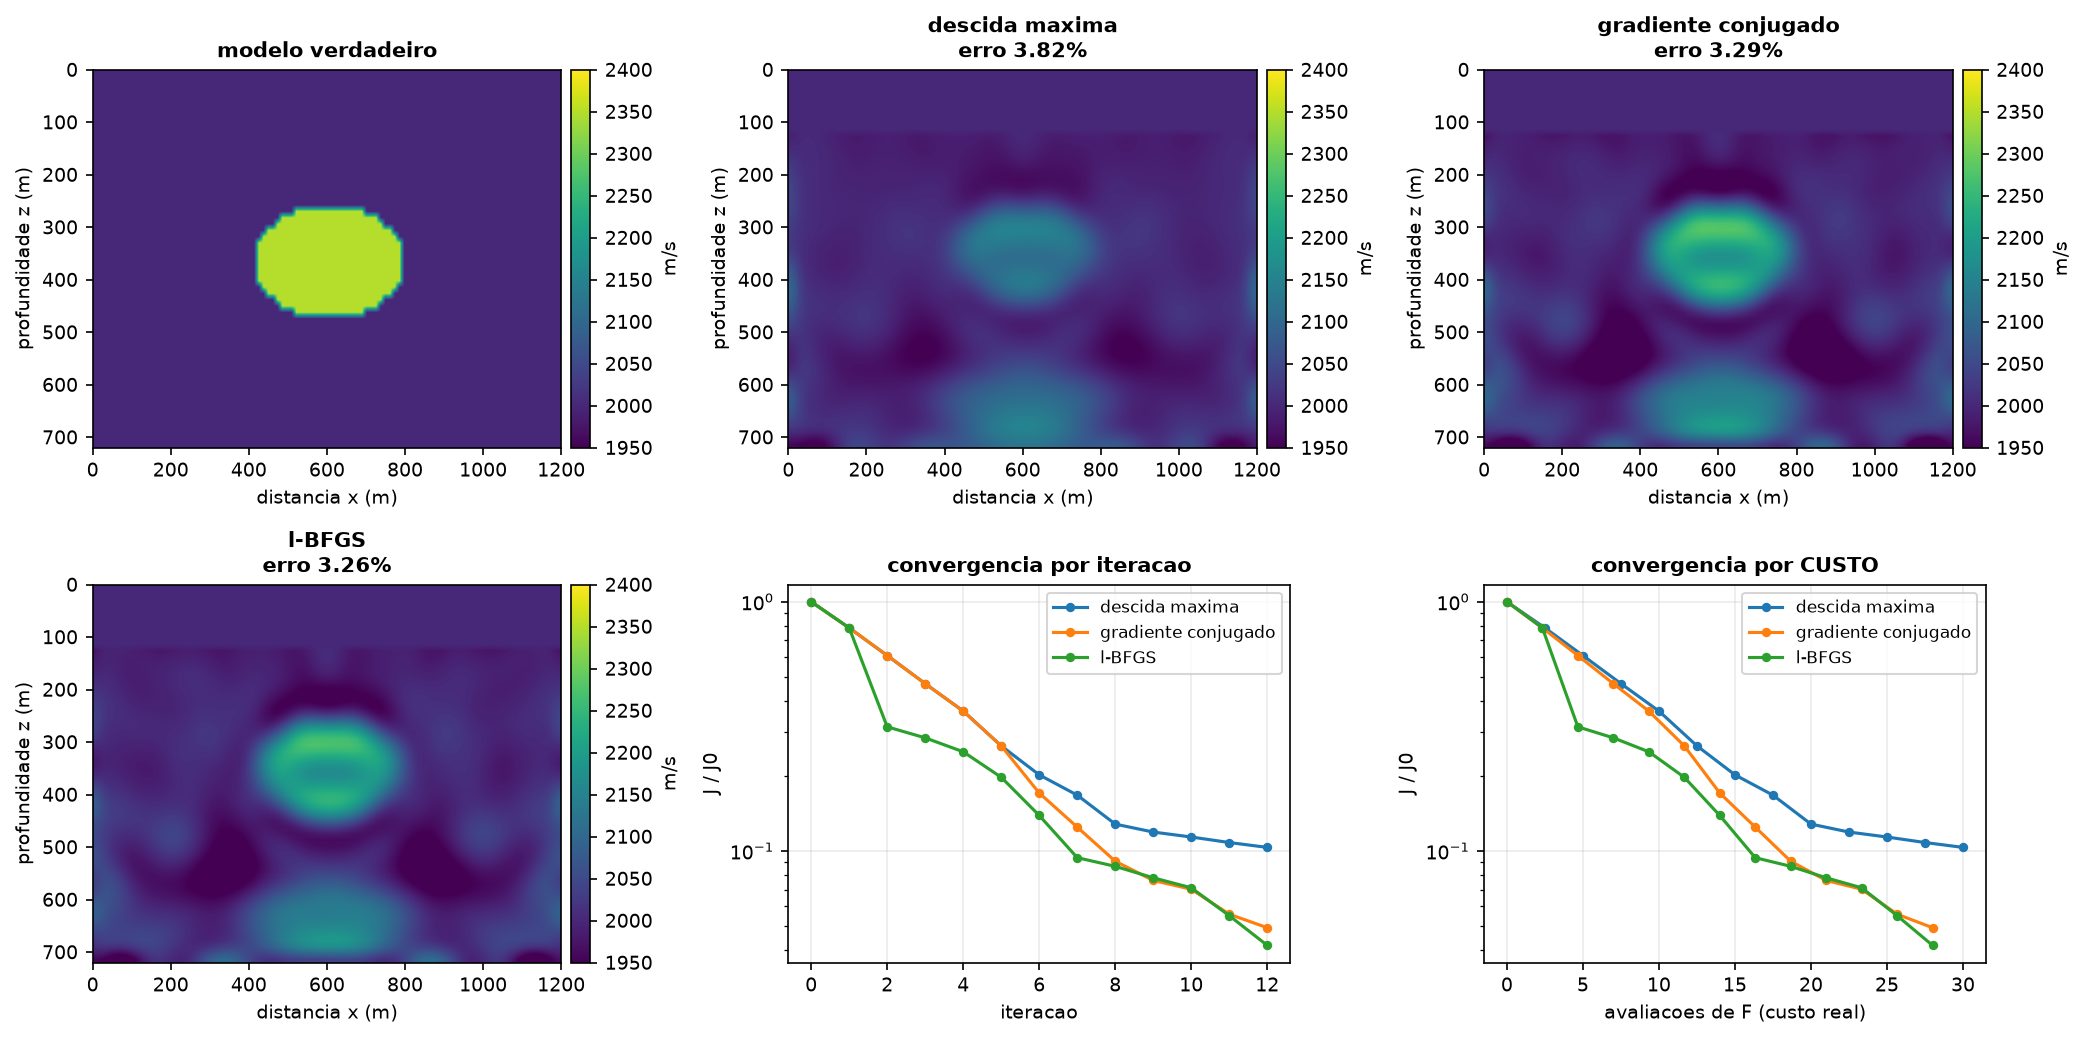
\includegraphics[width=0.96\textwidth]{../saidas/aula11/01_comparacao_otimizadores.png}
\caption{Compara\c{c}\~ao dos tr\^es otimizadores. Os dois pain\'eis
inferiores \`a direita contam hist\'orias diferentes: por itera\c{c}\~ao e por
custo.}
\end{figure}

\begin{atencao}[Compare por CUSTO, n\~ao por itera\c{c}\~ao]
Por \emph{itera\c{c}\~ao}, o l-BFGS quase sempre vence, porque cada
itera\c{c}\~ao usa curvatura acumulada. Por \emph{custo} --- n\'umero de
modelagens --- a compara\c{c}\~ao pode mudar, porque o n\'umero de
avalia\c{c}\~oes da busca linear varia de m\'etodo para m\'etodo. Neste
experimento ficou praticamente empatado (30, 28 e 28), mas n\~ao conte com
isso.

Sempre que comparar otimizadores num relat\'orio, mostre o eixo de custo.
\end{atencao}

\begin{exercicio}
\begin{enumerate}[leftmargin=*, itemsep=2pt]
\item Mostre que $\mathbf{g} = J'^{T}\mathbf{r}$ para
$J = \tfrac12\norm{\mathbf{r}}^{2}$, e identifique onde o estado adjunto
entra nessa express\~ao.
\item Por que rejeitar pares com $\inner{\mathbf{y}}{\mathbf{s}} \le 0$ no
l-BFGS?
\item A sua busca linear devolve $\alpha = 0$ na terceira itera\c{c}\~ao. Liste
tr\^es causas, em ordem de probabilidade.
\end{enumerate}
\textbf{Respostas.} (1) $\nabla_{\mvec}(\tfrac12\mathbf{r}^{T}\mathbf{r})
= (\partial\mathbf{r}/\partial\mvec)^{T}\mathbf{r} = J'^{T}\mathbf{r}$. O
estado adjunto \'e exatamente o algoritmo que aplica $J'^{T}$ a um vetor sem
formar $J'$. (2) Porque $\inner{\mathbf{y}}{\mathbf{s}} > 0$ \'e a
condi\c{c}\~ao que garante positividade definida da aproxima\c{c}\~ao, e
portanto que a dire\c{c}\~ao seja de descida. (3) Gradiente errado (verifique
primeiro); pr\'e-condicionamento exagerado deixando a dire\c{c}\~ao quase
ortogonal a $-\mathbf{g}$; hist\'orico do l-BFGS contaminado por uma troca de
banda sem reinicializa\c{c}\~ao.
\end{exercicio}

% =====================================================================
\chapter{A FWI completa: fluxo de trabalho}
\label{cap:completa}

\begin{ideia}
Um fluxo de FWI \'e uma sequ\^encia de decis\~oes, quase todas tomadas
\emph{antes} da primeira itera\c{c}\~ao. Este cap\'itulo monta o fluxo, e
mostra --- com n\'umeros medidos --- como ele pode falhar produzindo um
resultado que parece bom.
\end{ideia}

\section{O fluxo}

\begin{lstlisting}
# ---------- antes de qualquer inversao ----------
1. preparar dado:   remover onda direta (se nao modelada),
                    decidir sobre multiplas, estimar a wavelet
2. modelo inicial:  tomografia / analise de velocidade / pocos
3. dimensionar:     dh, dt, n_abs           (Caps. 3 e 4)
4. VERIFICAR o gradiente                    (Cap. 7)

# ---------- multiescala ----------
5. para cada banda f em [f_baixa ... f_alta]:
       d_filt = passa_baixa(d_obs, f)
       reiniciar historico do l-BFGS
       para it em 1..n_iter[f]:
           g = gradiente(m, d_filt)         # Cap. 6
           g = precondicionar(g)            # Cap. 8
           d = direcao(g, historico)        # Cap. 8
           a = busca_linear(m, d)           # Cap. 8
           m = projetar_na_caixa(m + a*d)   # Cap. 10

# ---------- depois ----------
6. diagnosticar e reportar                  (Caps. 9 e 12)
\end{lstlisting}

\begin{atencao}[A ordem dos passos 3 e 4 n\~ao \'e negoci\'avel]
Verificar o gradiente \emph{depois} de rodar a invers\~ao \'e in\'util: se ele
estava errado, tudo o que foi produzido at\'e ali precisa ser refeito. O
teste custa minutos (Cap.~\ref{cap:verificacao}).
\end{atencao}

\section{A ondaleta da fonte}

Em dado sint\'etico a fonte \'e conhecida. Em dado real, \textbf{n\~ao} --- e
um erro de ondaleta entra no res\'iduo exatamente como um erro de modelo.

A sa\'ida padr\~ao \'e estim\'a-la por m\'inimos quadrados, aproveitando que
$J$ \'e \emph{quadr\'atica} na ondaleta (o problema \'e linear nela, mesmo
sendo n\~ao linear em $\mvec$). No dom\'inio da frequ\^encia, para cada
$\omega$:
\begin{equation}
w(\omega) = \frac{\sum_{r} \overline{g_r(\omega)}\;d_{\text{obs},r}(\omega)}
                 {\sum_{r} \abs{g_r(\omega)}^{2} + \epsilon},
\label{eq:fonte}
\end{equation}
com $g_r(\omega)$ a resposta do modelo atual a uma fonte unit\'aria. Isto \'e,
na pr\'atica, um filtro de casamento entre sint\'etico e observado.

\begin{pratica}[Como usar \eqref{eq:fonte} sem se enganar]
Reestime a ondaleta \textbf{a cada troca de banda}, n\~ao a cada itera\c{c}\~ao
--- reestimar sempre deixa a fonte absorver o erro de modelo, e a invers\~ao
p\'ara de melhorar o modelo.

E desconfie de uma ondaleta estimada que muda muito entre bandas: isso indica
que ela est\'a compensando f\'isica faltante, n\~ao a assinatura da fonte.
\end{pratica}

\section{Um experimento controlado}

Mesmo modelo inicial, mesmo otimizador, \emph{mesmo n\'umero total de
itera\c{c}\~oes} (12). A \'unica diferen\c{c}a \'e a ordem em que a
informa\c{c}\~ao entra:

\begin{center}
\begin{tabular}{@{}lrrr@{}}
\toprule
\textbf{M\'etrica} & \textbf{Inicial} & \textbf{Mono (25\,Hz)}
& \textbf{Multi (5/12/25)} \\
\midrule
Erro relativo do modelo & 8{,}00\% & 7{,}35\% & \textbf{7{,}20\%} \\
Ganho sobre o inicial & --- & $+8{,}1\%$ & $+10{,}0\%$ \\
Correla\c{c}\~ao & 0{,}9333 & 0{,}9173 & 0{,}9296 \\
$R^{2}$ & 0{,}7284 & 0{,}7708 & \textbf{0{,}7799} \\
Tempo & --- & 3{,}8 min & 5{,}7 min \\
\bottomrule
\end{tabular}
\end{center}

Erro relativo dos \emph{dados}: $0{,}2573$ (inicial) $\to$ $0{,}0719$ (final).

\begin{atencao}[Leia este resultado com honestidade]
A vantagem da multiescala aqui \'e real mas \textbf{modesta} --- $0{,}15$
pontos percentuais. E isso \'e esperado: o pr\'oprio monoescala
\emph{melhorou} o modelo, sinal de que o inicial j\'a estava dentro do vale de
atra\c{c}\~ao de 25\,Hz. Quando o monoescala n\~ao sofre \emph{cycle
skipping}, n\~ao h\'a muito para o multiescala resgatar.

Note que isso \emph{n\~ao} se deduz dos 8\% por \eqref{eq:tolerancia}: a 25\,Hz,
com $c \approx 2300$\,m/s e percursos de 1--2\,km, a toler\^ancia seria de
2--5\%. A diferen\c{c}a \'e que \eqref{eq:tolerancia} fala de erro
\emph{cinem\'atico} acumulado no percurso, enquanto o erro relativo de modelo
\'e uma norma global que mistura todas as escalas --- um inicial suave pode ter
8\% de erro relativo e cinem\'atica quase certa.

Note tamb\'em a linha da correla\c{c}\~ao: ela \emph{piorou} em rela\c{c}\~ao
ao inicial nos dois casos, enquanto o erro relativo melhorou. M\'etricas
diferentes medem coisas diferentes --- por isso se reporta mais de uma.
\end{atencao}

\section{Estudo de robustez}

O teste que mede o valor real da estrat\'egia \'e degradar o inicial de
prop\'osito. Quatro modelos iniciais, com uma variante do mesmo fluxo (4 tiros
em vez de 6; 12 itera\c{c}\~oes no total em ambos os casos, de modo que os
n\'umeros n\~ao coincidem com os da tabela anterior):

\begin{center}
\begin{tabular}{@{}lrrrr@{}}
\toprule
\textbf{Modelo inicial} & \textbf{erro ini.} & \textbf{mono 25\,Hz}
& \textbf{multi 5/12/25} & \textbf{vantagem} \\
\midrule
linear suave           & 7{,}96\%  & 7{,}34\%  & \textbf{7{,}07\%}  & $+0{,}27$ pp \\
linear lento (viesado) & 16{,}68\% & \textbf{17{,}57\%} & \textbf{17{,}34\%} & $+0{,}24$ pp \\
constante              & 16{,}32\% & 16{,}10\% & 16{,}06\% & $+0{,}04$ pp \\
suavizado forte        & 4{,}95\%  & 4{,}01\%  & \textbf{3{,}70\%}  & $+0{,}31$ pp \\
\bottomrule
\end{tabular}
\end{center}

\begin{teoria}[Quatro leituras, e a segunda \'e a mais importante]
\textbf{Primeira:} a multiescala venceu em \emph{todos} os casos. A vantagem
\'e consistente, ainda que modesta nesta escala de problema.

\textbf{Segunda --- olhe a linha ``linear lento''.} O erro inicial era
$16{,}68\%$ e a FWI terminou em $17{,}57\%$ (mono) e $17{,}34\%$ (multi):
\textbf{a invers\~ao piorou o modelo}. Ela n\~ao travou, n\~ao deu erro, e a
fun\c{c}\~ao objetivo caiu direitinho. Convergiu para um m\'inimo local e, no
caminho, degradou o que j\'a se sabia.

Este \'e o fracasso mais perigoso da FWI, porque \emph{n\~ao se parece com
fracasso}. \'E por isso que reportar o erro do modelo \textbf{inicial} n\~ao
\'e formalidade.

\textbf{Terceira:} o melhor resultado absoluto ($3{,}70\%$) veio do inicial
``suavizado forte'' --- o modelo verdadeiro filtrado, inicial privilegiado que
s\'o existe em teste sint\'etico. Compare com ``constante'', que termina em
$16\%$: a diferen\c{c}a n\~ao est\'a no algoritmo, est\'a no que j\'a se sabia
antes de come\c{c}ar.

\textbf{Quarta --- a que contraria a expectativa:} a vantagem \emph{n\~ao}
cresceu quando o inicial piorou. Pela toler\^ancia \eqref{eq:tolerancia}, com
$c \approx 2300$\,m/s e percursos de 1 a 2\,km, o vale a 5\,Hz fica entre
$\sim$11\% e $\sim$23\%. Um erro de $\sim$16\% est\'a na borda desse vale, ou
fora dele, \emph{j\'a na primeira banda} --- e a\'i nenhuma ordem de bandas
salva. O rem\'edio seria come\c{c}ar em 2--3\,Hz, o que exige dado com energia
l\'a.
\end{teoria}

\begin{figure}[htbp]
\centering
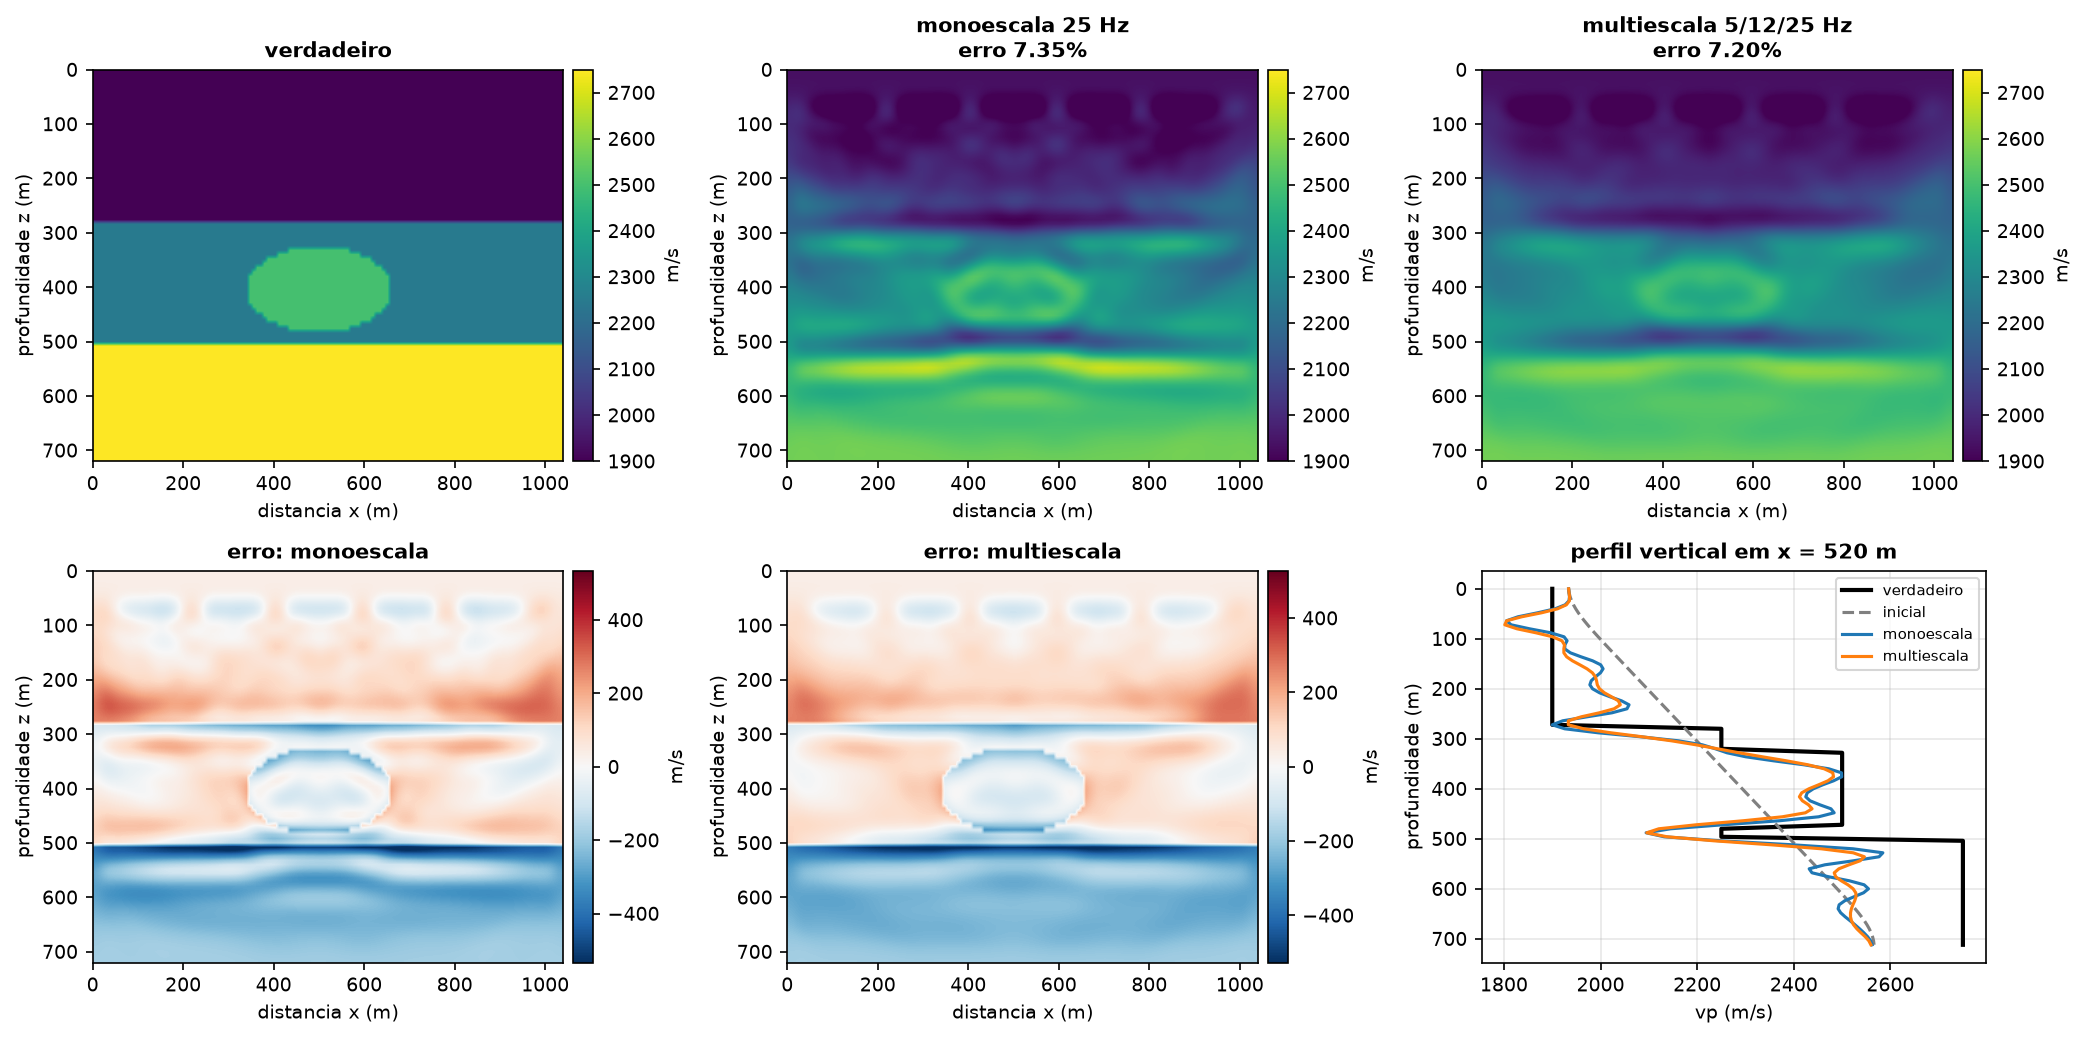
\includegraphics[width=0.96\textwidth]{../saidas/aula12/02_mono_vs_multi.png}
\caption{Monoescala \emph{versus} multiescala: modelos recuperados, mapas de
erro e perfil vertical.}
\end{figure}

\section{Como reportar uma FWI}

\begin{teoria}[O m\'inimo que sustenta uma conclus\~ao]
Uma figura de ``antes e depois'' n\~ao sustenta nada. Reporte:
\begin{itemize}[leftmargin=*, itemsep=1pt]
\item \textbf{erro relativo de modelo}
$\norm{\mvec_{\text{est}}-\mvec_{\text{verd}}}/\norm{\mvec_{\text{verd}}}$
--- e o mesmo n\'umero para o modelo \emph{inicial};
\item \textbf{curva de converg\^encia} de $J$, com eixo de \emph{custo};
\item \textbf{perfis verticais} comparando verdadeiro, inicial e invertido;
\item \textbf{mapa de erro} $\mvec_{\text{est}}-\mvec_{\text{verd}}$, que
revela \emph{onde} o m\'etodo falhou;
\item \textbf{compara\c{c}\~ao de sismogramas} observado $\times$ final, e o
\textbf{res\'iduo} --- ele \'e mais informativo que o valor de $J$.
\end{itemize}

Uma FWI que sai de 2\% para $1{,}5\%$ n\~ao demonstra quase nada; uma que sai
de 20\% para 5\% demonstra muito. Sem o ponto de partida, o n\'umero final
n\~ao significa nada.
\end{teoria}

% =====================================================================
\chapter{Regulariza\c{c}\~ao e informa\c{c}\~ao a priori}
\label{cap:regularizacao}

\begin{ideia}
Onde o dado n\~ao restringe o modelo, alguma coisa vai preencher o vazio.
Regularizar \'e escolher \emph{o qu\^e}, explicitamente, em vez de deixar a
escolha para o ru\'ido.
\end{ideia}

\begin{matematica}[problema mal posto, espa\c{c}o nulo, e a diferen\c{c}a entre $L_1$ e $L_2$]
\textbf{Bem posto}, no sentido de Hadamard, exige tr\^es coisas: a
solu\c{c}\~ao \emph{existe}, \'e \emph{\'unica}, e \emph{depende continuamente}
dos dados. A FWI falha nas duas \'ultimas --- e cada falha produz um sintoma
diferente.

\textbf{Falha de unicidade $\to$ espa\c{c}o nulo.} Se existe
$\delta\mvec \ne 0$ tal que $F(\mvec+\delta\mvec) = F(\mvec)$ (ou difere menos
que o ru\'ido), o dado \'e \emph{indiferente} a $\delta\mvec$. Esse conjunto de
dire\c{c}\~oes \'e o espa\c{c}o nulo pr\'atico do problema. Nele o gradiente
\'e nulo e o algoritmo n\~ao tem opini\~ao --- o valor final ali vem do modelo
inicial ou da regulariza\c{c}\~ao, \textbf{nunca do dado}.

\textbf{Falha de continuidade $\to$ amplifica\c{c}\~ao de ru\'ido.} Nas
dire\c{c}\~oes de sensibilidade pequena mas n\~ao nula, uma perturba\c{c}\~ao
min\'uscula no dado exige uma perturba\c{c}\~ao enorme no modelo: ru\'ido vira
estrutura de grande amplitude.

\textbf{Regularizar} \'e somar um termo que d\'a uma opini\~ao exatamente onde
o dado n\~ao tem nenhuma.

\medskip
\textbf{$L_1$ contra $L_2$: por que a escolha muda a geologia do resultado.}
Para um vetor de varia\c{c}\~oes $\mathbf{u}$,
\[
\norm{\mathbf{u}}_2^{2} = \sum_i u_i^{2},
\qquad
\norm{\mathbf{u}}_1 = \sum_i \abs{u_i} .
\]
Elevar ao quadrado pune \emph{desproporcionalmente} os valores grandes:
concentrar toda a varia\c{c}\~ao em um ponto fica car\'issimo, e dilu\'i-la
fica barato. A norma $L_1$ cobra o mesmo total dos dois jeitos.

Consequ\^encia: minimizar a $L_2$ da varia\c{c}\~ao produz solu\c{c}\~oes
\textbf{suaves}; minimizar a $L_1$ produz solu\c{c}\~oes \textbf{esparsas em
varia\c{c}\~ao} --- quase constantes por peda\c{c}os, com saltos n\'itidos.
\'E a mesma matem\'atica que, em outro contexto, faz o LASSO selecionar
poucas vari\'aveis.

\textbf{Derivada de um funcional integral.} Para
$R(m) = \int G(\nabla m)\dd\mathbf{x}$, perturbando $m \to m+\delta m$ e
integrando por partes,
\[
\delta R = -\int \nabla\!\cdot\!\left[
  \frac{\partial G}{\partial(\nabla m)}\right]\delta m\dd\mathbf{x}
\qquad\Longrightarrow\qquad
\nabla R = -\nabla\!\cdot\!\left[\frac{\partial G}{\partial(\nabla m)}\right].
\]
As duas f\'ormulas de gradiente da pr\'oxima se\c{c}\~ao s\~ao casos
particulares desta, com $G = \tfrac12\abs{\nabla m}^{2}$ e
$G = \abs{\nabla m}$.
\end{matematica}

\section{Por que regularizar}

A FWI \'e mal posta em dois sentidos. \textbf{Espa\c{c}o nulo}: existem
perturba\c{c}\~oes que praticamente n\~ao mudam os dados --- regi\~oes n\~ao
iluminadas, estruturas menores que $\lambda/2$, combina\c{c}\~oes de
par\^ametros que se cancelam. \textbf{Amplifica\c{c}\~ao de ru\'ido}: nas
dire\c{c}\~oes de baixa sensibilidade, um res\'iduo pequeno exige
perturba\c{c}\~ao grande do modelo.

\begin{equation}
J_{\text{total}}(\mvec) = J_{\text{dados}}(\mvec) + \lambda\,R(\mvec),
\qquad
\nabla J_{\text{total}} = \nabla J_{\text{dados}} + \lambda\,\nabla R .
\end{equation}

\begin{atencao}[Uma distin\c{c}\~ao que evita confus\~ao]
Regulariza\c{c}\~ao \textbf{n\~ao} existe para melhorar o ajuste dos dados:
comparando os minimizadores \emph{globais} com e sem ela, por
constru\c{c}\~ao, $J_{\text{dados}}$ s\'o pode ficar igual ou \emph{pior}. O
que ela faz \'e escolher, entre os muitos modelos que ajustam os dados
igualmente bem, aquele mais plaus\'ivel segundo um crit\'erio que \emph{voc\^e}
definiu.

(Num problema n\~ao convexo, com otimiza\c{c}\~ao local, a compara\c{c}\~ao
pr\'atica pode sair ao contr\'ario: partindo do mesmo inicial, a
regulariza\c{c}\~ao pode desviar a trajet\'oria de um m\'inimo local e terminar
com ajuste melhor --- Esser \emph{et al.} (2018) usam restri\c{c}\~oes de TV
exatamente com esse fim. \'E efeito de trajet\'oria, n\~ao de ajuste no
\'otimo.)

Isso significa que a escolha de $R$ \'e uma afirma\c{c}\~ao sobre a geologia,
e precisa ser justificada como tal.
\end{atencao}

\section{Tikhonov \emph{versus} Varia\c{c}\~ao Total}

\begin{align}
R_{\text{Tik}}(\mvec) &= \tfrac{1}{2}\int_{\Omega} \abs{\nabla m}^{2}\dd\mathbf{x},
  &\nabla R_{\text{Tik}} &= -\nabla^{2} m ,
  \label{eq:tik}\\[3pt]
R_{\text{TV}}(\mvec) &= \int_{\Omega} \abs{\nabla m}\dd\mathbf{x}
  \;\approx\; \int_{\Omega}\sqrt{\abs{\nabla m}^{2}+\varepsilon^{2}}\dd\mathbf{x},
  &\nabla R_{\text{TV}} &= -\nabla\!\cdot\!\left(
    \frac{\nabla m}{\sqrt{\abs{\nabla m}^{2}+\varepsilon^{2}}}\right).
  \label{eq:tv}
\end{align}

O $\varepsilon$ em \eqref{eq:tv} existe porque $\abs{\nabla m}$ n\~ao \'e
diferenci\'avel onde o gradiente se anula --- ou seja, em toda regi\~ao
homog\^enea, que \'e a maior parte do modelo. Escolha
$\varepsilon \sim 10^{-2}$ do contraste t\'ipico de $m$: grande demais e a TV
vira Tikhonov, pequeno demais e o gradiente fica inst\'avel.

\begin{teoria}[Por que $L_1$ preserva interfaces e $L_2$ n\~ao]
Compare o custo de acomodar uma varia\c{c}\~ao total de 1:

\begin{center}
\begin{tabular}{@{}lrr@{}}
\toprule
 & $L_2$ (Tikhonov) & $L_1$ (TV) \\
\midrule
Um salto de 1 em um ponto & 1{,}00 & 1{,}00 \\
A mesma varia\c{c}\~ao em 10 passos de 0{,}1 & \textbf{0{,}10} & 1{,}00 \\
\bottomrule
\end{tabular}
\end{center}

A $L_2$ \'e \emph{barata} para muitas varia\c{c}\~oes pequenas e cara para um
salto grande: por isso ela \textbf{suaviza}, borrando interfaces. A $L_1$ cobra
o mesmo nos dois casos: por isso tolera saltos n\'itidos enquanto ainda pune
oscila\c{c}\~ao de ru\'ido.

\textbf{Escolha:} alvo estratificado com contatos n\'itidos pede TV;
varia\c{c}\~ao gradual pede Tikhonov.
\end{teoria}

\subsection*{Vers\~ao anisotr\'opica}

Frequentemente se quer penalizar mais a varia\c{c}\~ao em uma dire\c{c}\~ao
que na outra --- t\'ipico em meio estratificado, onde a estrutura \'e
horizontal:
\begin{equation}
R = \tfrac{1}{2}\int \Bigl[a_x (\partial_x m)^{2}
  + a_z (\partial_z m)^{2}\Bigr]\dd\mathbf{x},
\qquad
\nabla R = -\bigl(a_x\,\partial_{xx} + a_z\,\partial_{zz}\bigr) m .
\end{equation}
Peso \textbf{maior} em $a_z$ penaliza mais a varia\c{c}\~ao \emph{vertical} e
produz um modelo mais suave na vertical. \'E f\'acil inverter os dois
na implementa\c{c}\~ao e obter exatamente o oposto do pretendido; verifique
com um modelo de teste que tenha estrutura s\'o em uma dire\c{c}\~ao.

\section{Um resultado que contraria a expectativa}

O experimento do curso usa dado com rela\c{c}\~ao sinal/ru\'ido de
\textbf{0\,dB} (ru\'ido com a mesma energia do sinal), 3 tiros e 18
itera\c{c}\~oes:

\begin{center}
\begin{tabular}{@{}lrr@{}}
\toprule
\textbf{Variante} & \textbf{Erro final} & \textbf{Correla\c{c}\~ao} \\
\midrule
modelo inicial & 4{,}75\% & 0{,}9554 \\
gradiente cru, sem regulariza\c{c}\~ao & 3{,}60\% & 0{,}9699 \\
gradiente cru + Tikhonov & 4{,}42\% & 0{,}9595 \\
gradiente cru + TV & 4{,}39\% & 0{,}9613 \\
\textbf{s\'o suaviza\c{c}\~ao do gradiente} & \textbf{3{,}56\%} & \textbf{0{,}9709} \\
\bottomrule
\end{tabular}
\end{center}

\begin{teoria}[Por que a regulariza\c{c}\~ao expl\'icita perdeu aqui]
O modelo inicial j\'a \'e suave, e com 18 itera\c{c}\~oes a invers\~ao n\~ao
tem tempo de gerar estrutura de alta frequ\^encia. O erro que sobra
\textbf{n\~ao \'e rugosidade}: \'e falta de \emph{contraste} --- os degraus de
velocidade ainda n\~ao foram recuperados em amplitude.

Tikhonov e TV penalizam exatamente o gradiente espacial, ou seja, penalizam o
contraste que ainda falta construir. Est\~ao puxando na dire\c{c}\~ao errada
\emph{para este problema}.

E note a \'ultima linha: apenas suavizando o gradiente, sem termo algum no
funcional, chega-se ao melhor resultado da tabela. Uma opera\c{c}\~ao de uma
linha.
\end{teoria}

\begin{pratica}[Regulariza\c{c}\~ao impl\'icita]
Existe muita regulariza\c{c}\~ao em FWI que raramente \'e reconhecida como
tal:
\begin{itemize}[leftmargin=*, itemsep=1pt]
\item suaviza\c{c}\~ao do gradiente a cada itera\c{c}\~ao;
\item modelo inicial suave --- ele j\'a restringe onde a solu\c{c}\~ao pode
chegar;
\item estrat\'egia multiescala --- as bandas baixas imp\~oem suavidade;
\item parada antecipada --- poucas itera\c{c}\~oes n\~ao produzem alta
frequ\^encia;
\item proje\c{c}\~ao em caixa.
\end{itemize}

Somar regulariza\c{c}\~ao expl\'icita a tudo isso frequentemente
\textbf{sobre-regulariza}. O sintoma \'e o da tabela: o modelo fica mais suave
e o erro \emph{aumenta}.

A conclus\~ao n\~ao \'e ``n\~ao use regulariza\c{c}\~ao'', e sim:
\textbf{diagnostique antes de escolher $R$}. Se o erro residual \'e
rugosidade, Tikhonov e TV ajudam; se \'e falta de contraste ou resolu\c{c}\~ao,
atrapalham.
\end{pratica}

\section{Escolhendo $\lambda$}

Calibre $\lambda$ de modo que $\lambda R$ valha uma fra\c{c}\~ao conhecida de
$J_{\text{dados}}$ no ponto inicial (2\%, por exemplo):
\begin{equation}
\lambda = \eta\,\frac{J_{\text{dados}}(\mvec_0)}{R(\mvec_0)},
\qquad \eta \approx 0{,}02 .
\end{equation}
Isso torna a escolha independente de unidades e reprodut\'ivel --- muito
melhor que testar pot\^encias de 10 \`as cegas.

Depois refine pela \textbf{curva em L}: para v\'arios $\lambda$, ponha
$J_{\text{dados}}$ em $x$ e $R$ em $y$, ambos em log. A curva tem forma de L,
e o $\lambda$ bom fica no \emph{cotovelo} --- o ponto de maior curvatura,
onde se deixa de comprar suavidade barata e se come\c{c}a a pagar com ajuste.

\begin{figure}[htbp]
\centering
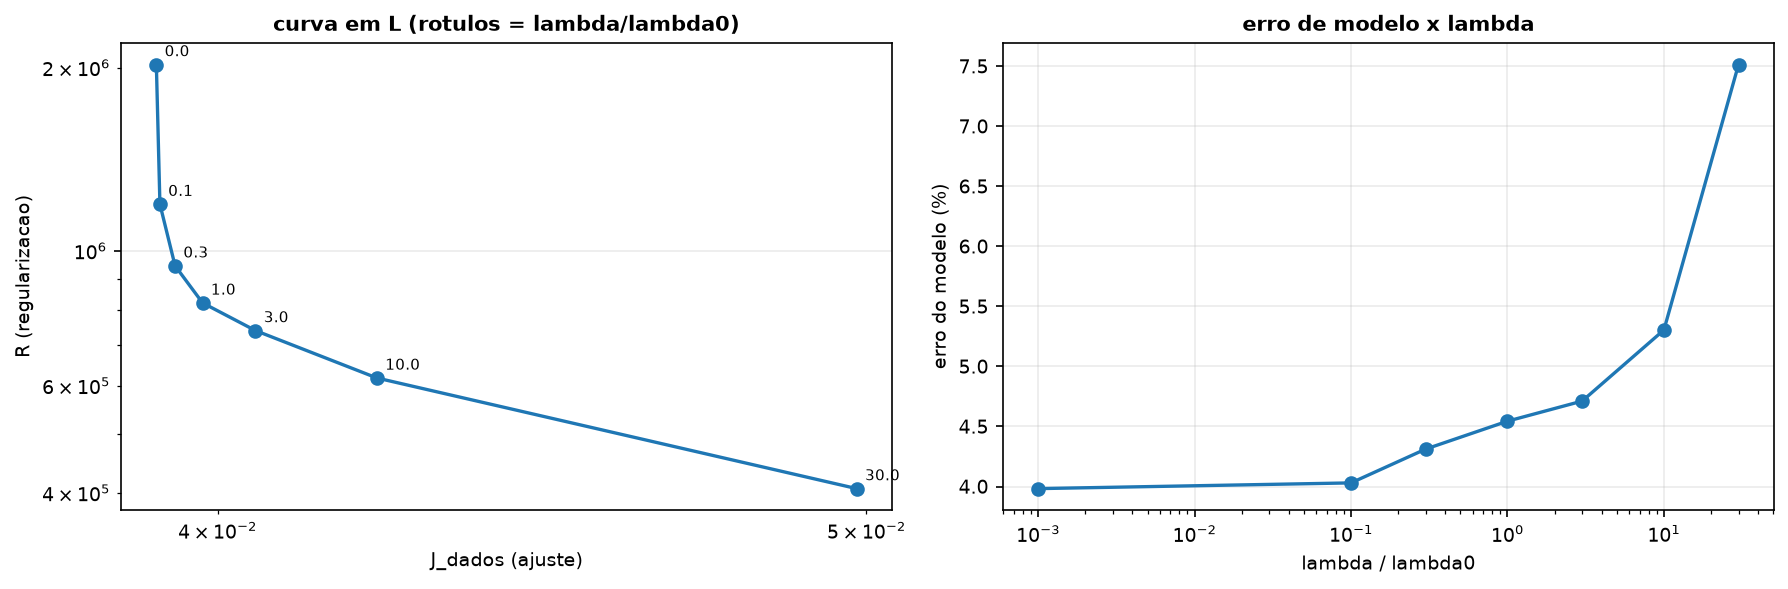
\includegraphics[width=0.78\textwidth]{../saidas/aula13/02_curva_em_L.png}
\caption{Curva em L medida pelo c\'odigo do curso ($J_{\text{dados}}$ no eixo
horizontal, $R$ no vertical; os r\'otulos s\~ao $\lambda/\lambda_0$). O cotovelo
\'e o compromisso: no ramo vertical, \`a esquerda ($\lambda$ pequeno), $R$
cresce sem ganho de ajuste --- ru\'ido entrando no modelo; no ramo horizontal,
\`a direita ($\lambda$ grande), sobre-regulariza\c{c}\~ao, com ajuste
sacrificado.}
\end{figure}

\begin{armadilha}[Uma exig\^encia de honestidade]
Em problema \emph{sint\'etico} voc\^e conhece o modelo verdadeiro e poderia
escolher $\lambda$ pelo menor erro de modelo. Em dado \textbf{real} isso \'e
imposs\'ivel --- voc\^e s\'o tem $J_{\text{dados}}$ e $R$. \'E para isso que
existe a curva em L.

Se reportar resultados escolhendo $\lambda$ pelo erro de modelo, diga isso
explicitamente. Caso contr\'ario o resultado parece melhor do que seria na
pr\'atica.
\end{armadilha}

\section{Modelo a priori e v\'inculos}

\begin{equation}
R_{\text{priori}}(\mvec) = \tfrac{1}{2}\,
\bigl\|W(\mvec-\mvec_{\text{priori}})\bigr\|^{2},
\qquad
\nabla R_{\text{priori}} = W^{T}W(\mvec - \mvec_{\text{priori}}).
\end{equation}

A matriz $W$ diz \emph{onde} voc\^e confia no modelo a priori. Uso
cl\'assico: peso alto ao longo de um po\c{c}o, onde h\'a perfil s\^onico
medido, e zero longe dele.

\begin{center}
\begin{tabular}{@{}lll@{}}
\toprule
\textbf{V\'inculo} & \textbf{Como} & \textbf{Quando} \\
\midrule
Caixa ($v_{\min}, v_{\max}$) & \texttt{clip} ap\'os cada passo & \textbf{sempre} \\
\'Agua fixa & zerar o gradiente na l\^amina d'\'agua & dado marinho \\
M\'ascara de profundidade & zerar abaixo da penetra\c{c}\~ao & evita artefato \\
Modelo a priori & $R = \norm{W(\mvec-\mvec_p)}^{2}$ & h\'a po\c{c}o/tomografia \\
Rela\c{c}\~ao entre par\^ametros & vincular $v_s,\rho$ a $v_p$ & multipar\^ametro \\
\bottomrule
\end{tabular}
\end{center}

\begin{atencao}[Onde clipar --- e \'e mais cedo do que se pensa]
Clipe \emph{tamb\'em dentro} da avalia\c{c}\~ao de $J$, e n\~ao apenas ap\'os
a atualiza\c{c}\~ao. A busca linear avalia $J(\mvec+\alpha\mathbf{d})$
\textbf{antes} de a proje\c{c}\~ao ser aplicada, e um passo exagerado pode
violar a CFL e estourar a simula\c{c}\~ao ali. O curso encontrou esse
\emph{overflow} exatamente assim.
\end{atencao}

\begin{exercicio}
\begin{enumerate}[leftmargin=*, itemsep=2pt]
\item Derive $\nabla R_{\text{Tik}} = -\nabla^{2}m$ a partir de
\eqref{eq:tik}.
\item Por que a TV precisa de $\varepsilon$, e o que acontece se
$\varepsilon$ for grande demais?
\item O seu res\'iduo final \'e dominado por oscila\c{c}\~ao de curto
comprimento de onda no modelo. Tikhonov, TV, ou nenhum dos dois?
\end{enumerate}
\textbf{Respostas.} (1) $\delta R = \int \nabla m\cdot\nabla\delta m
= -\int (\nabla^{2}m)\,\delta m$ ap\'os integrar por partes (termo de
fronteira nulo com condi\c{c}\~oes homog\^eneas), logo
$\nabla R = -\nabla^{2}m$. (2) Porque $\abs{\nabla m}$ n\~ao \'e
diferenci\'avel em $\nabla m = 0$, que \'e a situa\c{c}\~ao de toda regi\~ao
homog\^enea; com $\varepsilon \gg \abs{\nabla m}$,
$\sqrt{\abs{\nabla m}^2+\varepsilon^2} \approx \varepsilon +
\abs{\nabla m}^{2}/(2\varepsilon)$ --- a menos de uma constante, Tikhonov com
peso $1/\varepsilon$ --- e a TV degenera em Tikhonov. (3) Qualquer um dos dois
ajuda --- este \'e o caso em que a regulariza\c{c}\~ao \'e apropriada. TV se
voc\^e quiser preservar interfaces reais no meio da oscila\c{c}\~ao.
\end{exercicio}

% =====================================================================
\part*{\centering\color{azulfwi} Parte III --- Os limites}
\addcontentsline{toc}{part}{Parte III --- Os limites}

\chapter{Os limites da f\'isica adotada}
\label{cap:limites}

\begin{ideia}
Toda a Parte I adotou uma f\'isica simplificada. Este cap\'itulo apresenta a
fatura: quanto cada hip\'otese custa, como o custo aparece no resultado, e
como decidir se vale a pena pagar por f\'isica melhor.
\end{ideia}

\section{O invent\'ario de hip\'oteses}

\begin{center}
\begin{tabular}{@{}lll@{}}
\toprule
\textbf{Hip\'otese} & \textbf{Onde entrou} & \textbf{Quando quebra} \\
\midrule
$\mu = 0$ & Cap.~\ref{cap:fisica} & terrestre, contrastes de $v_s$ \\
densidade constante & Cap.~\ref{cap:fisica} & contrastes de imped\^ancia \\
sem atenua\c{c}\~ao ($Q\to\infty$) & Cap.~\ref{cap:fisica} & meio dissipativo,
  banda larga \\
isotropia & Cap.~\ref{cap:fisica} & folhelhos, fraturas \\
2D & volume inteiro & estrutura fora do plano \\
fonte conhecida & Cap.~\ref{cap:completa} & dado real: a ondaleta \'e estimada \\
ru\'ido gaussiano branco & Cap.~\ref{cap:misfit} & ru\'ido coerente, m\'ultiplas \\
\bottomrule
\end{tabular}
\end{center}

\begin{armadilha}[O princ\'ipio que vale mais que a tabela]
\textbf{O que a FWI n\~ao consegue explicar pela f\'isica, ela explica mexendo
no modelo.}

N\~ao existe v\'alvula de escape. Se o dado cont\'em um efeito que o operador
n\~ao reproduz, esse efeito entra inteiro no res\'iduo, e o gradiente o
converte em estrutura de velocidade. O modelo final absorve o erro de
f\'isica --- e parece um modelo, n\~ao um erro.
\end{armadilha}

\section{Limite 1: densidade e a ambiguidade da imped\^ancia}

O que controla a reflex\~ao n\~ao \'e a velocidade, \'e a \textbf{imped\^ancia}
$Z = \rho c$. Em incid\^encia normal,
\begin{equation}
R = \frac{Z_2 - Z_1}{Z_2 + Z_1}
  = \frac{\rho_2 c_2 - \rho_1 c_1}{\rho_2 c_2 + \rho_1 c_1}.
\end{equation}

\begin{center}
\begin{tabular}{@{}llr@{}}
\toprule
\textbf{Meio 1} & \textbf{Meio 2} & $R$ \\
\midrule
$c=2000,\ \rho=2{,}00$ & $c=2400,\ \rho=2{,}00$ & $+0{,}0909$ \\
$c=2000,\ \rho=2{,}00$ & $c=2000,\ \rho=2{,}40$ & $+0{,}0909$ \\
$c=2000,\ \rho=2{,}00$ & $c=2400,\ \rho=1{,}67$ & $+0{,}0010$ \\
\bottomrule
\end{tabular}
\end{center}

As duas primeiras linhas produzem \emph{exatamente} a mesma reflex\~ao por
causas diferentes. A terceira \'e pior: velocidade 20\% maior com densidade
17\% menor d\'a reflex\~ao praticamente \textbf{nula} em incid\^encia normal ---
nas reflex\~oes de afastamento curto, a interface n\~ao aparece. Ela s\'o \'e
vista pela cinem\'atica das ondas que a atravessam, ou pela varia\c{c}\~ao de
$R$ com o \^angulo, que exige afastamento.

\'E o exemplo mais limpo de ambiguidade velocidade--densidade, e a raiz do
\emph{crosstalk} em invers\~ao multipar\^ametro.

\ponte{N\'ivel 3, §2.3 e Cap.\ 11}{o tratamento quantitativo disso: padr\~oes de
radia\c{c}\~ao, que mostram \emph{em quais \^angulos} cada par\^ametro
imprime a sua assinatura --- e portanto que aquisi\c{c}\~ao os separa.}

\section{Limite 2: elasticidade}

Medido no Cap\'itulo~\ref{cap:fisica}: a diferen\c{c}a entre o sismograma
el\'astico e o ac\'ustico tem norma \textbf{compar\'avel \`a do pr\'oprio
dado}. S\~ao ondas S e convers\~oes P--S. Essa energia n\~ao some do dado
real: ou voc\^e a modela, ou a remove no processamento, ou ela vai para o
res\'iduo.

\begin{center}
\begin{tabular}{@{}llll@{}}
\toprule
\textbf{Extens\~ao} & \textbf{Par\^ametros} & \textbf{Custo} & \textbf{Resolve} \\
\midrule
Ac\'ustica & $v_p$ & 1$\times$ & cinem\'atica P \\
Ac\'ustica $+\rho$ & $v_p,\rho$ & 1$\times$ & amplitude de reflex\~ao \\
Viscoac\'ustica & $v_p,Q$ & 2--4$\times$ & dissipa\c{c}\~ao e dispers\~ao \\
El\'astica & $v_p,v_s,\rho$ & 3--5$\times$ & ondas S, convers\~oes, AVO \\
Viscoel\'astica & $+Q_p,Q_s$ & 6--10$\times$ & tudo acima \\
Anisotr\'opica (VTI) & $+\epsilon,\delta$ & 2--3$\times$ & folhelhos \\
\bottomrule
\end{tabular}
\end{center}

\begin{atencao}[Os fatores de custo s\~ao na mesma malha]
A malha \'e dimensionada pela \emph{menor} velocidade (receita do
Cap.~\ref{cap:numerico}), e na el\'astica ela \'e $v_s$. Como o
custo 2D escala com $\Delta h^{-3}$ e o 3D com $\Delta h^{-4}$, a raz\~ao
$v_p/v_s$ entra \emph{al\'em} do fator da tabela: com $v_p/v_s = 2$, mais
$8\times$ em 2D e $16\times$ em 3D. Em sedimento raso e mole, com $v_s$ muito
baixo, a diferen\c{c}a chega a ordens de grandeza.
\end{atencao}

\section{Limite 3: atenua\c{c}\~ao e o fator $Q$}

\begin{matematica}[causalidade, e por que ela amarra amplitude a fase]
Este \'e o ponto conceitual mais importante do cap\'itulo, e vale prepar\'a-lo
antes de qualquer f\'ormula.

\textbf{Resposta em frequ\^encia.} Um meio linear age sobre uma onda
multiplicando cada componente de frequ\^encia por um n\'umero complexo: o
m\'odulo muda a \emph{amplitude}, o argumento muda a \emph{fase}. Atenuar \'e
reduzir o m\'odulo; atrasar \'e girar o argumento.

\textbf{Causalidade.} Nenhum sinal pode chegar antes de ser emitido. Isso
parece \'obvio e tem uma consequ\^encia matem\'atica forte: se a resposta \'e
causal, a sua transformada \'e anal\'itica num semiplano complexo de
frequ\^encia (o inferior, com a conven\c{c}\~ao de Fourier deste volume; o
superior, com a conven\c{c}\~ao oposta $e^{+\mathrm{i}\omega t}$, comum em
f\'isica), e as partes real e imagin\'aria deixam de ser independentes --- ficam ligadas pelas
rela\c{c}\~oes de \textbf{Kramers--Kronig}, que expressam uma como integral da
outra.

\textbf{O que isso significa em portugu\^es.} Voc\^e \emph{n\~ao pode}
projetar um meio que absorva energia de forma dependente da frequ\^encia e
n\~ao mude a velocidade de fase. As duas coisas s\~ao a mesma coisa vista de
dois \^angulos. Dissipa\c{c}\~ao e dispers\~ao v\^em sempre juntas.

\textbf{Lei de pot\^encia.} Adiante aparece $c(\omega) \propto
\omega^{\gamma}$ com $\gamma$ min\'usculo ($\sim 10^{-3}$). Uma pot\^encia com
expoente t\~ao pequeno \'e quase uma constante --- e \'e justamente por isso
que o efeito passa despercebido em modelagem, e reaparece como erro de tempo
de tr\^ansito acumulado em percursos longos.
\end{matematica}

O fator de qualidade $Q$ \'e, aproximadamente, o n\'umero de ciclos que uma
onda percorre antes de a amplitude cair por $e^{-\pi}$. Valores t\'ipicos:
\'agua $>1000$; rocha consolidada 100--300; sedimento n\~ao consolidado
20--50; sedimento raso saturado ou com g\'as 10--30.

\begin{teoria}[Dissipa\c{c}\~ao e dispers\~ao s\~ao insepar\'aveis]
Consequ\^encia pr\'atica da caixa acima: \textbf{n\~ao adianta ``corrigir a
amplitude'' de um dado atenuado e continuar usando uma equa\c{c}\~ao sem
perdas.} Ao atenuar, o meio tamb\'em mudou a \emph{fase} --- e a FWI \'e um
m\'etodo governado por fase. Um operador sem dissipa\c{c}\~ao est\'a errado nas
duas contas ao mesmo tempo.
\end{teoria}

\subsection*{O modelo constant-$Q$ de Kjartansson}

Entre as representa\c{c}\~oes da dissipa\c{c}\~ao, a de Kjartansson (1979) \'e
a mais usada quando se quer $Q$ aproximadamente constante na banda
s\'ismica. Ela parte de uma lei constitutiva de pot\^encia, e o expoente se
relaciona a $Q$ por
\begin{equation}
\gamma = \frac{1}{\pi}\arctan\!\left(\frac{1}{Q}\right),
\label{eq:gamma}
\end{equation}
com velocidade de fase e amplitude dadas por
\begin{equation}
c(\omega) = c_0\left(\frac{\omega}{\omega_{\text{ref}}}\right)^{\gamma},
\qquad
A(\omega) = \exp\!\left[-\frac{\omega L}{2\,Q\,c(\omega)}\right].
\label{eq:kjartansson}
\end{equation}

\begin{atencao}[Precis\~ao da forma usada]
O fator de atenua\c{c}\~ao em \eqref{eq:kjartansson} usa $1/(2Q)$, v\'alido
para $Q \gg 1$. A forma exata de Kjartansson traz $\tan(\pi\gamma/2)$ no
lugar. A diferen\c{c}a medida \'e de $0{,}25\%$ em $Q=10$ e $0{,}06\%$ em
$Q=20$ --- irrelevante na faixa s\'ismica, mas vale saber que a express\~ao
\'e uma aproxima\c{c}\~ao.
\end{atencao}

No dom\'inio do tempo, essa depend\^encia de pot\^encia conduz a operadores de
ordem \textbf{fracion\'aria} --- por isso a implementa\c{c}\~ao viscoac\'ustica
\'e substancialmente mais trabalhosa que a ac\'ustica, e costuma ser feita com
laplacianos fracion\'arios ou com uma soma de mecanismos de relaxa\c{c}\~ao
(modelo SLS).

\subsection*{O que $Q$ faz com um pulso}

Aplicando \eqref{eq:kjartansson} a uma Ricker de $f_0 = 20$\,Hz,
$c_0 = 2000$\,m/s, $L = 1500$\,m (frequ\^encia de pico do espectro
cont\'inuo; a FFT da aula~14, com resolu\c{c}\~ao de $0{,}24$\,Hz, arredonda o
caso $Q = 200$ para $18{,}8$\,Hz):

\begin{center}
\begin{tabular}{@{}rrrr@{}}
\toprule
$Q$ & $\gamma$ & \textbf{amplitude rel.} & $f$ de pico (Hz) \\
\midrule
$10\,000$ & $3{,}2\times10^{-5}$ & 1{,}0000 & 20{,}0 \\
200 & $1{,}59\times10^{-3}$ & 0{,}7738 & 18{,}9 \\
100 & $3{,}18\times10^{-3}$ & 0{,}6008 & 17{,}8 \\
50  & $6{,}37\times10^{-3}$ & 0{,}3713 & 15{,}9 \\
20  & $1{,}59\times10^{-2}$ & 0{,}1056 & 11{,}5 \\
\bottomrule
\end{tabular}
\end{center}

\begin{figure}[htbp]
\centering
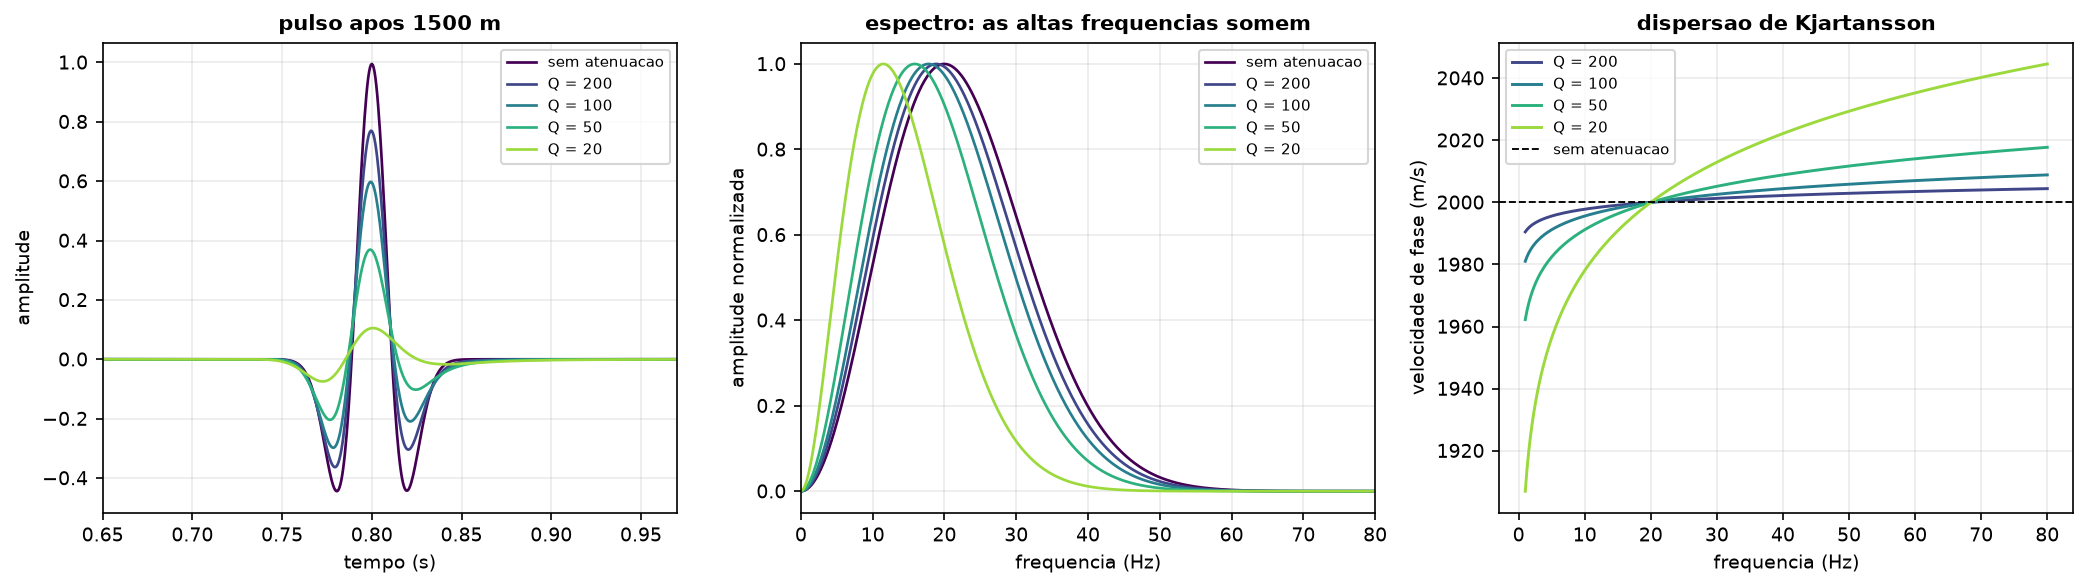
\includegraphics[width=0.96\textwidth]{../saidas/aula14/01_atenuacao_kjartansson.png}
\caption{Efeito do modelo constant-$Q$: pulso no tempo, espectro e
dispers\~ao da velocidade de fase. Tr\^es efeitos simult\^aneos, nenhum
presente na equa\c{c}\~ao ac\'ustica.}
\end{figure}

\subsection*{Quando ignorar $Q$ provoca \emph{cycle skipping}}

Aqui as pe\c{c}as do volume se encaixam. Modelando com $c_0$ constante mas
tendo dado de um meio dispersivo, o erro de tempo de tr\^ansito \'e
\begin{equation}
\delta t(f) = \frac{L}{c_0} - \frac{L}{c(f)}
 = \frac{L}{c_0}\left[1 - \left(\frac{f}{f_{\text{ref}}}\right)^{-\gamma}\right],
\end{equation}
e o crit\'erio de meio ciclo \eqref{eq:meiociclo} decide se isso importa:

\begin{center}
\begin{tabular}{@{}rrrrrl@{}}
\toprule
$Q$ & $L$ (m) & $f$ (Hz) & $\abs{\delta t}$ (ms) & $T/2$ (ms) & \\
\midrule
100 & 1000 & 10 & 1{,}10 & 50{,}0 & ok \\
100 & 6000 & 60 & 10{,}47 & 8{,}3 & \textbf{cycle skipping} \\
50  & 6000 & 60 & 20{,}91 & 8{,}3 & \textbf{cycle skipping} \\
20  & 1000 & 60 & 8{,}66 & 8{,}3 & \textbf{cycle skipping} \\
20  & 6000 & 10 & 33{,}25 & 50{,}0 & ok \\
10  & 6000 & 10 & 66{,}70 & 50{,}0 & \textbf{cycle skipping} \\
10  & 6000 & 60 & 102{,}76 & 8{,}3 & \textbf{cycle skipping} \\
\bottomrule
\end{tabular}
\end{center}
{\small ($c_0 = 2000$\,m/s, $f_{\text{ref}} = 20$\,Hz)}

O padr\~ao \'e claro: o risco cresce com percurso \emph{longo}, frequ\^encia
\emph{alta} e $Q$ \emph{baixo}, os tr\^es juntos. Com $Q = 200$ e percursos
curtos, a aproxima\c{c}\~ao sem perdas \'e perfeitamente defens\'avel.

\begin{atencao}[O que a tabela n\~ao cobre]
Ela contabiliza apenas o erro de \emph{fase} por dispers\~ao. O erro de
\emph{amplitude} por dissipa\c{c}\~ao \'e adicional, e afeta diretamente
qualquer funcional que compare amplitudes --- como o $L_2$ usado no volume
inteiro.
\end{atencao}

\subsection*{O adjunto de um meio dissipativo}
\label{sec:adjunto-visco}

\begin{teoria}[Duas coisas que costumam ser confundidas]
A equa\c{c}\~ao ac\'ustica sem perdas \'e auto-adjunta, e por isso o mesmo
propagador serve para o direto e para o adjunto. Com atenua\c{c}\~ao isso
muda, e \'e preciso separar dois enunciados:

\textbf{(1) A propaga\c{c}\~ao adjunta \'e est\'avel.} O operador
viscoac\'ustico cont\'em uma derivada \emph{primeira} no tempo, e
$\partial_t^{*} = -\partial_t$. Quando o problema adjunto \'e escrito na
vari\'avel de tempo revertida $\tau = T - t$, essa troca de sinal se cancela
com a invers\~ao do sentido do tempo: o campo adjunto obedece a uma
equa\c{c}\~ao \emph{dissipativa} em $\tau$, e integra-se sem problema.

\textbf{(2) Reconstruir o campo \emph{direto} de tr\'as para frente \'e que
explode.} A t\'ecnica de economia de mem\'oria que recupera o campo direto
propagando-o ao contr\'ario a partir do estado final exige rodar a
dissipa\c{c}\~ao \emph{ao contr\'ario} --- isto \'e, amplificar. Isso
amplifica tamb\'em o erro de arredondamento, exponencialmente.

Conclus\~ao pr\'atica: em meio atenuante, use \emph{checkpointing} para o
campo direto. N\~ao \'e o adjunto que \'e inst\'avel; \'e a reconstru\c{c}\~ao
do direto.
\end{teoria}

\section{Como decidir qual f\'isica voc\^e precisa}

A decis\~ao se faz olhando para o dado e para o \textbf{res\'iduo}, n\~ao por
gosto nem por disponibilidade de c\'odigo.

\begin{enumerate}[leftmargin=*]
\item \textbf{Olhe o res\'iduo}, n\~ao s\'o o valor de $J$. Res\'iduo com
estrutura \emph{coerente} \'e a assinatura de f\'isica faltando. Res\'iduo que
parece ru\'ido aleat\'orio significa que voc\^e chegou ao limite do dado.
\item \textbf{Compare espectros} de observado e sint\'etico em fun\c{c}\~ao do
afastamento. Se o sint\'etico mant\'em alta frequ\^encia que o dado real j\'a
perdeu em afastamentos longos, h\'a atenua\c{c}\~ao n\~ao modelada.
\item \textbf{Verifique amplitude $\times$ afastamento.} Decaimento mais
r\'apido no dado real aponta dissipa\c{c}\~ao ou espalhamento.
\item \textbf{Procure eventos ausentes.} Energia no dado real em tempos onde o
sint\'etico ac\'ustico n\~ao produz nada: ondas S, convers\~oes ou m\'ultiplas.
\item \textbf{Teste a sensibilidade.} Gere dado sint\'etico com a f\'isica mais
completa e inverta com a mais simples. O erro de modelo resultante \'e a
medida direta do custo da aproxima\c{c}\~ao --- e o experimento mais
informativo que existe para justificar (ou dispensar) uma extens\~ao.
\end{enumerate}

\begin{armadilha}[O caminho inverso tamb\'em tem custo]
Adicionar f\'isica sem necessidade traz mais par\^ametros, mais
\emph{crosstalk}, mais m\'inimos locais, mais tempo de m\'aquina e mais
dificuldade em atribuir um resultado a uma causa.

Uma FWI ac\'ustica bem feita, com bom modelo inicial e multiescala honesta,
costuma render mais que uma viscoel\'astica mal condicionada. A pergunta certa
n\~ao \'e ``qual a f\'isica mais completa?'', e sim \textbf{``qual \'e a
f\'isica mais simples que explica o meu dado?''}
\end{armadilha}

% =====================================================================
\chapter{Diagn\'ostico}
\label{cap:diagnostico}

\begin{ideia}
FWI quase nunca falha com uma mensagem de erro: falha produzindo um resultado
bonito. Este cap\'itulo \'e a lista de sintomas, a causa de cada um, e a ordem
em que investigar.
\end{ideia}

\section{A FWI n\~ao converge ($J$ n\~ao cai)}
\begin{enumerate}[leftmargin=*]
\item O gradiente est\'a correto? Rode o teste de Taylor
(Cap.~\ref{cap:verificacao}). \textbf{Antes de qualquer outra coisa.}
\item A busca linear est\'a retornando $\alpha = 0$? A dire\c{c}\~ao n\~ao \'e
de descida --- verifique $\inner{\mathbf{g}}{\mathbf{d}} < 0$.
\item O sinal do gradiente est\'a certo? Compare $-\mathbf{g}$ com uma
perturba\c{c}\~ao conhecida, e confira em qual par\^ametro ele est\'a escrito
(Eq.~\ref{eq:cadeia}).
\item O passo inicial \'e razo\'avel? Deve alterar o modelo em 1--3\%.
\end{enumerate}

\section{$J$ cai mas o modelo est\'a errado}
\begin{enumerate}[leftmargin=*]
\item \textbf{Cycle skipping.} Recomece de uma frequ\^encia mais baixa. Se o
resultado mudar, era isso.
\item Modelo inicial fora do vale de atra\c{c}\~ao --- verifique com
\eqref{eq:tolerancia}.
\item F\'isica faltando: o res\'iduo final tem estrutura coerente?
\item Bordas: artefatos de reflex\~ao entrando no res\'iduo.
\item Ondaleta da fonte mal estimada: ela absorve erro de modelo e trava o
progresso.
\end{enumerate}

\section{S\'o a parte rasa \'e atualizada}
\begin{enumerate}[leftmargin=*]
\item Falta m\'ascara na faixa de fonte/receptor.
\item Falta compensa\c{c}\~ao de ilumina\c{c}\~ao
(Cap.~\ref{cap:otimizacao}).
\item Afastamento insuficiente para a profundidade desejada --- e isso nenhum
ajuste de algoritmo resolve.
\end{enumerate}

\section{O campo estoura (\texttt{NaN})}
\begin{enumerate}[leftmargin=*]
\item CFL: $c_{\max}\Delta t/\Delta h$ acima do limite \eqref{eq:cfl}.
\item O modelo saiu da caixa f\'isica durante a busca linear --- clipe
\emph{tamb\'em dentro} da avalia\c{c}\~ao de $J$.
\end{enumerate}

\section{Cauda oscilat\'oria onde n\~ao deveria haver evento}
\begin{enumerate}[leftmargin=*]
\item Dispers\~ao num\'erica: $G$ insuficiente. Reduza $\Delta h$, aumente a
ordem espacial, ou baixe $f_0$.
\item Se $G$ j\'a est\'a alto e o problema persiste: \textbf{\'e o $\Delta t$}
--- reduza $C$ (veja a caixa da §3.3).
\item Confirme sempre com uma simula\c{c}\~ao em meio homog\^eneo.
\end{enumerate}

\section{As cinco perguntas antes de acreditar num resultado}

\begin{teoria}[]
\begin{enumerate}[leftmargin=*, itemsep=2pt]
\item \textbf{Qual era o erro do modelo inicial?} Sem isso, o erro final n\~ao
significa nada.
\item \textbf{O gradiente foi verificado?} Se n\~ao, nada mais na lista
importa.
\item \textbf{O res\'iduo final parece ru\'ido ou tem estrutura?} Estrutura
coerente indica f\'isica faltando, n\~ao converg\^encia.
\item \textbf{O resultado muda se eu come\c{c}ar de uma frequ\^encia mais
baixa?} Se muda, o primeiro resultado estava num m\'inimo local.
\item \textbf{O resultado muda se eu come\c{c}ar de outro modelo inicial?} Se
muda muito, quem est\'a determinando a resposta \'e o modelo inicial, n\~ao o
dado.
\end{enumerate}
\end{teoria}

% =====================================================================
\appendix

\chapter{Nota\c{c}\~ao}

\begin{center}
\begin{longtable}{@{}ll@{}}
\toprule
\textbf{S\'imbolo} & \textbf{Significado} \\
\midrule
\endhead
$\mvec$ & vetor de par\^ametros do modelo \\
$m = 1/c^{2}$ & vagarosidade ao quadrado (par\^ametro de invers\~ao) \\
$c$, $v_p$ & velocidade de onda P (m/s) \\
$v_s$ & velocidade de onda S (m/s) \\
$\rho$ & densidade \\
$\lambda, \mu$ & par\^ametros de Lam\'e ($\mu$ = m\'odulo de cisalhamento) \\
$K$ & m\'odulo de compressibilidade \\
$p$ & press\~ao \\
$\sigma_{ij}$ & tensor de tens\~oes \\
$F$ & operador de modelagem direta \\
$J'$ & jacobiana $\partial\mathbf{r}/\partial\mvec$ (matriz de sensibilidade) \\
$J$ & funcional objetivo \\
$\mathbf{r}$ & vetor residual \\
$\mathbf{g}$ & gradiente \\
$H$, $H_{\text{GN}}$ & Hessiana e sua aproxima\c{c}\~ao de Gauss--Newton \\
$\lambda(\mathbf{x},t)$ & campo adjunto (multiplicador de Lagrange) \\
$\alpha$ & comprimento do passo \\
$\Delta h$, $\Delta t$ & espa\c{c}amento da malha e passo de tempo \\
$C$, $C_{\lim}$ & n\'umero de Courant e seu limite \\
$G$ & pontos por comprimento de onda \\
$S(\theta)$ & s\'imbolo do est\^encil espacial \\
$f_0$ & frequ\^encia de pico da fonte \\
$Q$ & fator de qualidade \\
$\gamma$ & expoente de Kjartansson \\
$E$ & operador de extens\~ao do modelo para a moldura \\
\bottomrule
\end{longtable}
\end{center}

\begin{atencao}[Tr\^es colis\~oes de s\'imbolo, herdadas da literatura]
$\lambda$ \'e par\^ametro de Lam\'e (Cap.~\ref{cap:fisica}), campo adjunto
(Cap.~\ref{cap:adjunto}), peso de regulariza\c{c}\~ao
(Cap.~\ref{cap:regularizacao}) \emph{e} comprimento de onda. $J$ \'e o
funcional e $J'$ a jacobiana do \emph{res\'iduo}, n\~ao a derivada de $J$.
$\mu$ \'e m\'odulo de cisalhamento. O contexto resolve, mas vale saber que a
colis\~ao \'e da \'area, n\~ao deste texto.
\end{atencao}

\chapter{F\'ormulas de bolso}

\begin{center}
\begin{longtable}{@{}p{5.3cm}p{9.6cm}@{}}
\toprule
\textbf{Para} & \textbf{Use} \\
\midrule
\endhead
Banda da fonte & $f_{\max} \approx 2{,}5 f_0$ (malha);
  $f \approx 1{,}6 f_0$ (resolu\c{c}\~ao) \\
Resolu\c{c}\~ao & $\delta_{\min} \approx \lambda/2 = c/2f$ \\
Penetra\c{c}\~ao & $z_{\max} \approx x_{\text{off}}^{\max}/6$ a
  $x_{\text{off}}^{\max}/3$ \\
Malha & $\Delta h = c_{\min}/(G f_{\max})$, $G = 8$ (O4) ou 5 (O8) \\
Passo de tempo & $\Delta t = 0{,}9\,C_{\lim}\Delta h/c_{\max}$;
  $C_{\lim} = 0{,}61$ (O4), $0{,}55$ (O8) em 2D \\
Moldura & $n_{abs} \ge 0{,}5\,c_{\max}/(f_{\min}\Delta h)$ \\
Amostragem de receptores & $\Delta x_{\text{rec}} < c_{\text{ap}}/2f_{\max}$ \\
Toler\^ancia do modelo inicial & $\abs{\delta c} < c^{2}/(2 f L)$ \\
Gradiente & $\partial J/\partial m = \int_0^T \lambda\,\partial_{tt}p\dd t$,
  discreto com peso $\Delta h^{2}\Delta t$ \\
Convers\~ao de par\^ametro & $\partial J/\partial c
  = (-2/c^{3})\,\partial J/\partial m$ \\
Passo inicial & $\alpha_0 = 0{,}02\max\abs{\mvec}/\max\abs{\mathbf{d}}$ \\
Peso de regulariza\c{c}\~ao & $\lambda = 0{,}02\,
  J_{\text{dados}}(\mvec_0)/R(\mvec_0)$, refinado pela curva em L \\
Custo total & $n_{\text{iter}} n_{\text{bandas}} n_{\text{tiros}}
  \cdot (2+n_{\text{busca}})$ modelagens \\
Kjartansson & $\gamma = \arctan(1/Q)/\pi$;
  $c(\omega) = c_0(\omega/\omega_{\text{ref}})^{\gamma}$ \\
\bottomrule
\end{longtable}
\end{center}

\chapter{Refer\^encias}

\begin{enumerate}[leftmargin=*, itemsep=3pt]
\item ASNAASHARI, A.; BROSSIER, R.; GARAMBOIS, S.; AUDEBERT, F.; THORE, P.;
VIRIEUX, J.
\emph{Regularized seismic full waveform inversion with prior model
information.} Geophysics, v.~78, n.~2, p.~R25--R36, 2013.

\item BUNKS, C.; SALECK, F.~M.; ZALESKI, S.; CHAVENT, G.
\emph{Multiscale seismic waveform inversion.} Geophysics, v.~60, n.~5,
p.~1457--1473, 1995.

\item CARCIONE, J.~M. \emph{Wave Fields in Real Media.} 4.~ed. Elsevier, 2022.

\item CERJAN, C.; KOSLOFF, D.; KOSLOFF, R.; RESHEF, M. \emph{A nonreflecting
boundary condition for discrete acoustic and elastic wave equations.}
Geophysics, v.~50, n.~4, p.~705--708, 1985.

\item ESSER, E.; GUASCH, L.; VAN LEEUWEN, T.; ARAVKIN, A.~Y.; HERRMANN, F.~J.
\emph{Total variation regularization strategies in full-waveform inversion.}
SIAM Journal on Imaging Sciences, v.~11, n.~1, p.~376--406, 2018.

\item KJARTANSSON, E. \emph{Constant-Q wave propagation and attenuation.}
Journal of Geophysical Research, v.~84, p.~4737--4748, 1979.

\item KREBS, J.~R. \emph{et al.} \emph{Fast full-wavefield seismic inversion
using encoded sources.} Geophysics, v.~74, n.~6, p.~WCC177--WCC188, 2009.

\item MARDAN, A.; GIROUX, B.; FABIEN-OUELLET, G. \emph{PyFWI: A Python package
for full-waveform inversion and reservoir monitoring.} SoftwareX, v.~22,
art.~101384, 2023.

\item MORGAN, J. \emph{et al.} \emph{Next-generation seismic experiments:
wide-angle, multi-azimuth, three-dimensional, full-waveform inversion.}
Geophysical Journal International, v.~195, n.~3, p.~1657--1678, 2013.

\item NOCEDAL, J.; WRIGHT, S.~J. \emph{Numerical Optimization.} 2.~ed.
Springer, 2006.

\item PLESSIX, R.-E. \emph{A review of the adjoint-state method for computing
the gradient of a functional with geophysical applications.} Geophysical
Journal International, v.~167, n.~2, p.~495--503, 2006.

\item SHIN, C.; JANG, S.; MIN, D.-J. \emph{Improved amplitude preservation for
prestack depth migration by inverse scattering theory.} Geophysical
Prospecting, v.~49, n.~5, p.~592--606, 2001.

\item TARANTOLA, A. \emph{Inversion of seismic reflection data in the acoustic
approximation.} Geophysics, v.~49, n.~8, p.~1259--1266, 1984.

\item VIRIEUX, J.; OPERTO, S. \emph{An overview of full-waveform inversion in
exploration geophysics.} Geophysics, v.~74, n.~6, p.~WCC1--WCC26, 2009.

\item VIRIEUX, J.; ASNAASHARI, A.; BROSSIER, R.; M\'ETIVIER, L.; RIBODETTI,
A.; ZHOU, W. \emph{An introduction to full waveform inversion.} In:
\emph{Encyclopedia of Exploration Geophysics}. Tulsa: Society of Exploration
Geophysicists, 2014. p.~R1-1--R1-40. DOI 10.1190/1.9781560803027.entry6.
\end{enumerate}

\vfill
\begin{center}
{\color{cianofwi}\rule{0.55\textwidth}{1pt}}\\[0.35cm]
{\small Volume 2 de 3 $\cdot$ os tr\^es volumes compartilham a mesma estrutura
de cap\'itulos.\\
Figuras e n\'umeros gerados pelo c\'odigo em \arq{aulas/} e \arq{fwikit/}.}
\end{center}

\end{document}
